\documentclass[twoside]{book}

% Packages required by doxygen
\usepackage{calc}
\usepackage{doxygen}
\usepackage{graphicx}
\usepackage[utf8]{inputenc}
\usepackage{makeidx}
\usepackage{multicol}
\usepackage{multirow}
\usepackage{textcomp}
\usepackage[table]{xcolor}

% NLS support packages
\usepackage[french]{babel}

% Font selection
\usepackage[T1]{fontenc}
\usepackage{mathptmx}
\usepackage[scaled=.90]{helvet}
\usepackage{courier}
\usepackage{amssymb}
\usepackage{sectsty}
\renewcommand{\familydefault}{\sfdefault}
\allsectionsfont{%
  \fontseries{bc}\selectfont%
  \color{darkgray}%
}
\renewcommand{\DoxyLabelFont}{%
  \fontseries{bc}\selectfont%
  \color{darkgray}%
}

% Page & text layout
\usepackage{geometry}
\geometry{%
  a4paper,%
  top=2.5cm,%
  bottom=2.5cm,%
  left=2.5cm,%
  right=2.5cm%
}
\tolerance=750
\hfuzz=15pt
\hbadness=750
\setlength{\emergencystretch}{15pt}
\setlength{\parindent}{0cm}
\setlength{\parskip}{0.2cm}
\makeatletter
\renewcommand{\paragraph}{%
  \@startsection{paragraph}{4}{0ex}{-1.0ex}{1.0ex}{%
    \normalfont\normalsize\bfseries\SS@parafont%
  }%
}
\renewcommand{\subparagraph}{%
  \@startsection{subparagraph}{5}{0ex}{-1.0ex}{1.0ex}{%
    \normalfont\normalsize\bfseries\SS@subparafont%
  }%
}
\makeatother

% Headers & footers
\usepackage{fancyhdr}
\pagestyle{fancyplain}
\fancyhead[LE]{\fancyplain{}{\bfseries\thepage}}
\fancyhead[CE]{\fancyplain{}{}}
\fancyhead[RE]{\fancyplain{}{\bfseries\leftmark}}
\fancyhead[LO]{\fancyplain{}{\bfseries\rightmark}}
\fancyhead[CO]{\fancyplain{}{}}
\fancyhead[RO]{\fancyplain{}{\bfseries\thepage}}
\fancyfoot[LE]{\fancyplain{}{}}
\fancyfoot[CE]{\fancyplain{}{}}
\fancyfoot[RE]{\fancyplain{}{\bfseries\scriptsize Généré le Lundi 1 Décembre 2014 19\-:08\-:18 pour Tales Of The Northern Land par Doxygen }}
\fancyfoot[LO]{\fancyplain{}{\bfseries\scriptsize Généré le Lundi 1 Décembre 2014 19\-:08\-:18 pour Tales Of The Northern Land par Doxygen }}
\fancyfoot[CO]{\fancyplain{}{}}
\fancyfoot[RO]{\fancyplain{}{}}
\renewcommand{\footrulewidth}{0.4pt}
\renewcommand{\chaptermark}[1]{%
  \markboth{#1}{}%
}
\renewcommand{\sectionmark}[1]{%
  \markright{\thesection\ #1}%
}

% Indices & bibliography
\usepackage{natbib}
\usepackage[titles]{tocloft}
\setcounter{tocdepth}{3}
\setcounter{secnumdepth}{5}
\makeindex

% Hyperlinks (required, but should be loaded last)
\usepackage{ifpdf}
\ifpdf
  \usepackage[pdftex,pagebackref=true]{hyperref}
\else
  \usepackage[ps2pdf,pagebackref=true]{hyperref}
\fi
\hypersetup{%
  colorlinks=true,%
  linkcolor=blue,%
  citecolor=blue,%
  unicode%
}

% Custom commands
\newcommand{\clearemptydoublepage}{%
  \newpage{\pagestyle{empty}\cleardoublepage}%
}


%===== C O N T E N T S =====

\begin{document}

% Titlepage & ToC
\hypersetup{pageanchor=false}
\pagenumbering{roman}
\begin{titlepage}
\vspace*{7cm}
\begin{center}%
{\Large Tales Of The Northern Land \\[1ex]\large 0.\-3 }\\
\vspace*{1cm}
{\large Généré par Doxygen 1.8.6}\\
\vspace*{0.5cm}
{\small Lundi 1 Décembre 2014 19:08:18}\\
\end{center}
\end{titlepage}
\clearemptydoublepage
\tableofcontents
\clearemptydoublepage
\pagenumbering{arabic}
\hypersetup{pageanchor=true}

%--- Begin generated contents ---
\chapter{Tales\-Of\-The\-Northern\-Land}
\label{md_README}
\hypertarget{md_README}{}
Projet d'objet et developpement d'applications L3

Tactical-\/\-R\-P\-G avec des elements d'idle games 
\chapter{Liste des bogues}
\label{bug}
\hypertarget{bug}{}

\begin{DoxyRefList}
\item[\label{bug__bug000001}%
\hypertarget{bug__bug000001}{}%
Membre \hyperlink{classCreateurPersonnage_a53a8e0403bd828add3bc1189cc7b4916}{Createur\-Personnage\-:\-:texte\-Classe} ()]pas fini \-:(  
\item[\label{bug__bug000002}%
\hypertarget{bug__bug000002}{}%
Membre \hyperlink{classPersonnage_ae9f35f04c2e15c98d97db9675d531d46}{Personnage\-:\-:change\-Posture} ()]need un delete de la posture ? 
\end{DoxyRefList}
\chapter{Index hiérarchique}
\section{Hiérarchie des classes}
Cette liste d'héritage est classée approximativement par ordre alphabétique \-:\begin{DoxyCompactList}
\item \contentsline{section}{Afficheur}{\pageref{classAfficheur}}{}
\item \contentsline{section}{Branche}{\pageref{classBranche}}{}
\item \contentsline{section}{Classe}{\pageref{classClasse}}{}
\begin{DoxyCompactList}
\item \contentsline{section}{Classe\-Divine}{\pageref{classClasseDivine}}{}
\item \contentsline{section}{Classe\-Heroique}{\pageref{classClasseHeroique}}{}
\item \contentsline{section}{Classe\-Parangon}{\pageref{classClasseParangon}}{}
\end{DoxyCompactList}
\item \contentsline{section}{Createur\-Personnage}{\pageref{classCreateurPersonnage}}{}
\item \contentsline{section}{Generateur\-Personnage}{\pageref{classGenerateurPersonnage}}{}
\item \contentsline{section}{Instancieur}{\pageref{classInstancieur}}{}
\item \contentsline{section}{Item}{\pageref{classItem}}{}
\begin{DoxyCompactList}
\item \contentsline{section}{Arme}{\pageref{classArme}}{}
\begin{DoxyCompactList}
\item \contentsline{section}{Decorator}{\pageref{classDecorator}}{}
\begin{DoxyCompactList}
\item \contentsline{section}{Amelioration\-Critique}{\pageref{classAmeliorationCritique}}{}
\item \contentsline{section}{Amelioration\-Degat}{\pageref{classAmeliorationDegat}}{}
\item \contentsline{section}{Amelioration\-Precision}{\pageref{classAmeliorationPrecision}}{}
\end{DoxyCompactList}
\item \contentsline{section}{Epee}{\pageref{classEpee}}{}
\item \contentsline{section}{Lance}{\pageref{classLance}}{}
\item \contentsline{section}{Sort}{\pageref{classSort}}{}
\end{DoxyCompactList}
\end{DoxyCompactList}
\item \contentsline{section}{Marchand}{\pageref{classMarchand}}{}
\item \contentsline{section}{Personnage}{\pageref{classPersonnage}}{}
\item \contentsline{section}{Posture}{\pageref{classPosture}}{}
\begin{DoxyCompactList}
\item \contentsline{section}{Attaquant}{\pageref{classAttaquant}}{}
\item \contentsline{section}{Defenseur}{\pageref{classDefenseur}}{}
\item \contentsline{section}{Soigneur}{\pageref{classSoigneur}}{}
\item \contentsline{section}{Tacticien}{\pageref{classTacticien}}{}
\end{DoxyCompactList}
\item \contentsline{section}{Race}{\pageref{classRace}}{}
\item \contentsline{section}{Technique}{\pageref{classTechnique}}{}
\begin{DoxyCompactList}
\item \contentsline{section}{Technique\-Statistique}{\pageref{classTechniqueStatistique}}{}
\end{DoxyCompactList}
\end{DoxyCompactList}

\chapter{Index des classes}
\section{Liste des classes}
Liste des classes, structures, unions et interfaces avec une brève description \-:\begin{DoxyCompactList}
\item\contentsline{section}{\hyperlink{classAfficheur}{Afficheur} }{\pageref{classAfficheur}}{}
\item\contentsline{section}{\hyperlink{classAmeliorationCritique}{Amelioration\-Critique} }{\pageref{classAmeliorationCritique}}{}
\item\contentsline{section}{\hyperlink{classAmeliorationDegat}{Amelioration\-Degat} }{\pageref{classAmeliorationDegat}}{}
\item\contentsline{section}{\hyperlink{classAmeliorationPrecision}{Amelioration\-Precision} }{\pageref{classAmeliorationPrecision}}{}
\item\contentsline{section}{\hyperlink{classArme}{Arme} }{\pageref{classArme}}{}
\item\contentsline{section}{\hyperlink{classAttaquant}{Attaquant} }{\pageref{classAttaquant}}{}
\item\contentsline{section}{\hyperlink{classBranche}{Branche} }{\pageref{classBranche}}{}
\item\contentsline{section}{\hyperlink{classClasse}{Classe} }{\pageref{classClasse}}{}
\item\contentsline{section}{\hyperlink{classClasseDivine}{Classe\-Divine} }{\pageref{classClasseDivine}}{}
\item\contentsline{section}{\hyperlink{classClasseHeroique}{Classe\-Heroique} }{\pageref{classClasseHeroique}}{}
\item\contentsline{section}{\hyperlink{classClasseParangon}{Classe\-Parangon} }{\pageref{classClasseParangon}}{}
\item\contentsline{section}{\hyperlink{classCreateurPersonnage}{Createur\-Personnage} }{\pageref{classCreateurPersonnage}}{}
\item\contentsline{section}{\hyperlink{classDecorator}{Decorator} }{\pageref{classDecorator}}{}
\item\contentsline{section}{\hyperlink{classDefenseur}{Defenseur} }{\pageref{classDefenseur}}{}
\item\contentsline{section}{\hyperlink{classEpee}{Epee} }{\pageref{classEpee}}{}
\item\contentsline{section}{\hyperlink{classGenerateurPersonnage}{Generateur\-Personnage} }{\pageref{classGenerateurPersonnage}}{}
\item\contentsline{section}{\hyperlink{classInstancieur}{Instancieur} }{\pageref{classInstancieur}}{}
\item\contentsline{section}{\hyperlink{classItem}{Item} }{\pageref{classItem}}{}
\item\contentsline{section}{\hyperlink{classLance}{Lance} }{\pageref{classLance}}{}
\item\contentsline{section}{\hyperlink{classMarchand}{Marchand} }{\pageref{classMarchand}}{}
\item\contentsline{section}{\hyperlink{classPersonnage}{Personnage} }{\pageref{classPersonnage}}{}
\item\contentsline{section}{\hyperlink{classPosture}{Posture} }{\pageref{classPosture}}{}
\item\contentsline{section}{\hyperlink{classRace}{Race} }{\pageref{classRace}}{}
\item\contentsline{section}{\hyperlink{classSoigneur}{Soigneur} }{\pageref{classSoigneur}}{}
\item\contentsline{section}{\hyperlink{classSort}{Sort} }{\pageref{classSort}}{}
\item\contentsline{section}{\hyperlink{classTacticien}{Tacticien} }{\pageref{classTacticien}}{}
\item\contentsline{section}{\hyperlink{classTechnique}{Technique} }{\pageref{classTechnique}}{}
\item\contentsline{section}{\hyperlink{classTechniqueStatistique}{Technique\-Statistique} }{\pageref{classTechniqueStatistique}}{}
\end{DoxyCompactList}

\chapter{Documentation des classes}
\hypertarget{classAfficheur}{\section{Référence de la classe Afficheur}
\label{classAfficheur}\index{Afficheur@{Afficheur}}
}
\subsection*{Fonctions membres publiques}
\begin{DoxyCompactItemize}
\item 
\hypertarget{classAfficheur_a007dbdbc0894dbf96db2cea82af9577b}{\hyperlink{classAfficheur_a007dbdbc0894dbf96db2cea82af9577b}{Afficheur} ()}\label{classAfficheur_a007dbdbc0894dbf96db2cea82af9577b}

\begin{DoxyCompactList}\small\item\em Constructeur. \end{DoxyCompactList}\item 
\hypertarget{classAfficheur_a9b0194e4c1c7bd3a818f8a2725fe73b0}{\hyperlink{classAfficheur_a9b0194e4c1c7bd3a818f8a2725fe73b0}{$\sim$\-Afficheur} ()}\label{classAfficheur_a9b0194e4c1c7bd3a818f8a2725fe73b0}

\begin{DoxyCompactList}\small\item\em Destructeur. \end{DoxyCompactList}\item 
void \hyperlink{classAfficheur_abf9d4a2be48a5347a7b9faf440cb5f35}{afficher\-Persos} (\hyperlink{classPersonnage}{Personnage} $\ast$perso1, \hyperlink{classPersonnage}{Personnage} $\ast$perso2)
\begin{DoxyCompactList}\small\item\em afficher les statistiques de deux personnages \end{DoxyCompactList}\item 
void \hyperlink{classAfficheur_ae7cc6b7ab9167866261941632227bd0e}{afficher\-Perso} (\hyperlink{classPersonnage}{Personnage} $\ast$perso1)
\begin{DoxyCompactList}\small\item\em afficher le statistique d'un personnage \end{DoxyCompactList}\end{DoxyCompactItemize}


\subsection{Documentation des fonctions membres}
\hypertarget{classAfficheur_ae7cc6b7ab9167866261941632227bd0e}{\index{Afficheur@{Afficheur}!afficher\-Perso@{afficher\-Perso}}
\index{afficher\-Perso@{afficher\-Perso}!Afficheur@{Afficheur}}
\subsubsection[{afficher\-Perso}]{\setlength{\rightskip}{0pt plus 5cm}void Afficheur\-::afficher\-Perso (
\begin{DoxyParamCaption}
\item[{{\bf Personnage} $\ast$}]{perso1}
\end{DoxyParamCaption}
)}}\label{classAfficheur_ae7cc6b7ab9167866261941632227bd0e}


afficher le statistique d'un personnage 

On limite la taille des noms de classe et de perso a 7 pour eviter un derp de l'affichage 
\begin{DoxyParams}{Paramètres}
{\em Personnage$\ast$} & perso1 le perso a afficher \\
\hline
\end{DoxyParams}
\hypertarget{classAfficheur_abf9d4a2be48a5347a7b9faf440cb5f35}{\index{Afficheur@{Afficheur}!afficher\-Persos@{afficher\-Persos}}
\index{afficher\-Persos@{afficher\-Persos}!Afficheur@{Afficheur}}
\subsubsection[{afficher\-Persos}]{\setlength{\rightskip}{0pt plus 5cm}void Afficheur\-::afficher\-Persos (
\begin{DoxyParamCaption}
\item[{{\bf Personnage} $\ast$}]{perso1, }
\item[{{\bf Personnage} $\ast$}]{perso2}
\end{DoxyParamCaption}
)}}\label{classAfficheur_abf9d4a2be48a5347a7b9faf440cb5f35}


afficher les statistiques de deux personnages 

On limite la taille des noms de classe et de perso a 7 pour eviter un derp de l'affichage 
\begin{DoxyParams}{Paramètres}
{\em Personnage$\ast$} & perso1 le perso afficher a gauche \\
\hline
{\em Personnage$\ast$} & perso2 le perso afficher a droite \\
\hline
\end{DoxyParams}


La documentation de cette classe a été générée à partir des fichiers suivants \-:\begin{DoxyCompactItemize}
\item 
Afficheur.\-hpp\item 
Afficheur.\-cpp\end{DoxyCompactItemize}

\hypertarget{classAmeliorationCritique}{\section{Référence de la classe Amelioration\-Critique}
\label{classAmeliorationCritique}\index{Amelioration\-Critique@{Amelioration\-Critique}}
}
Graphe d'héritage de Amelioration\-Critique\-:\begin{figure}[H]
\begin{center}
\leavevmode
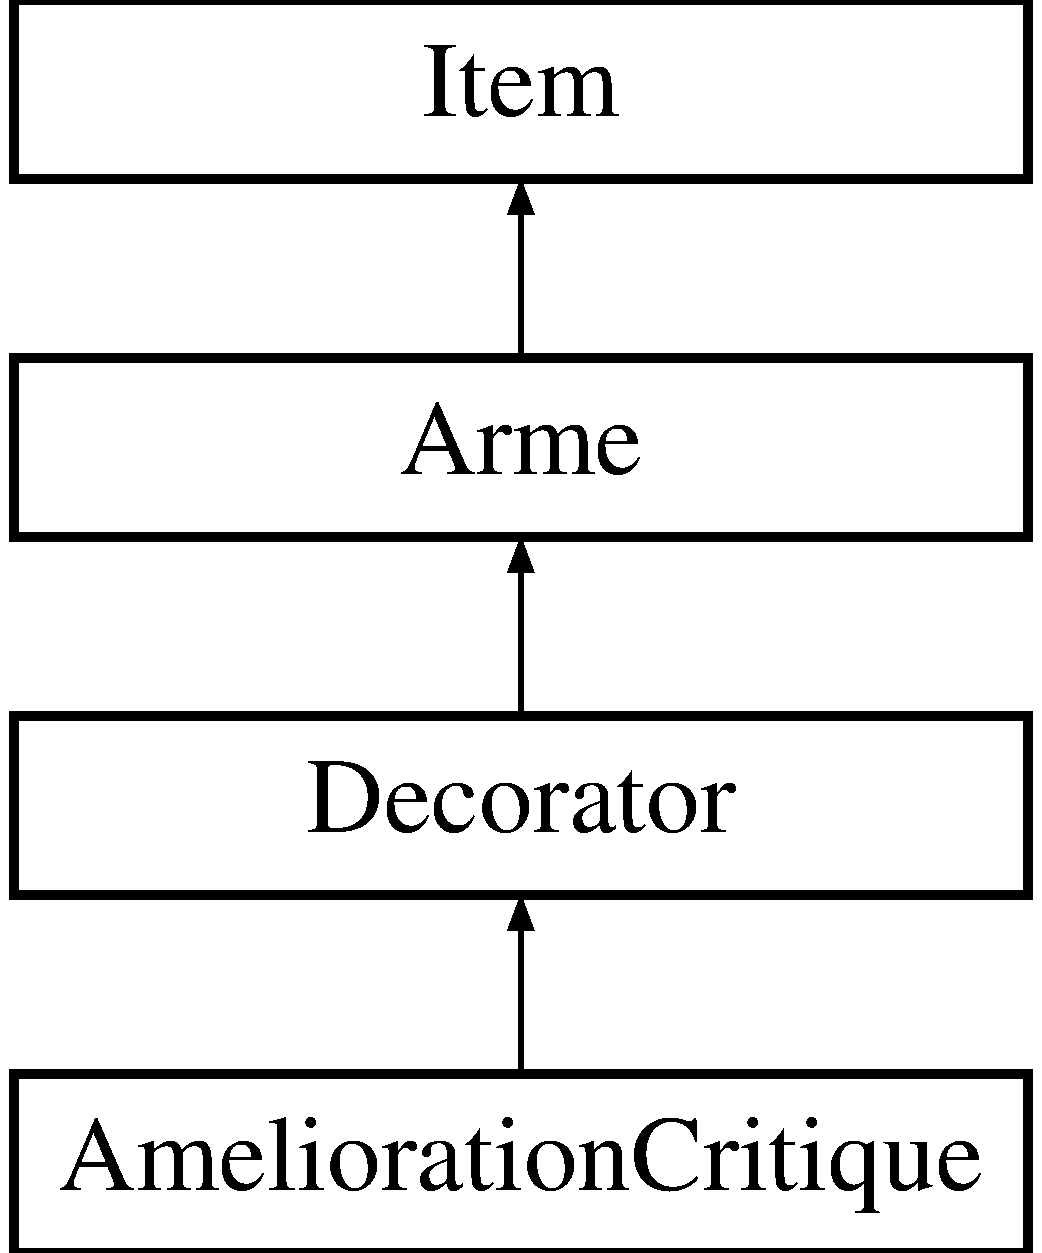
\includegraphics[height=4.000000cm]{classAmeliorationCritique}
\end{center}
\end{figure}
\subsection*{Fonctions membres publiques}
\begin{DoxyCompactItemize}
\item 
\hyperlink{classAmeliorationCritique_a51aa1a46f887621eeb228e0b4fb95ec1}{Amelioration\-Critique} (\hyperlink{classArme}{Arme} $\ast$arme)
\begin{DoxyCompactList}\small\item\em Décorateur de critique modifiant le pourcentage critique de l'arme. \end{DoxyCompactList}\end{DoxyCompactItemize}
\subsection*{Membres hérités additionnels}


\subsection{Documentation des constructeurs et destructeur}
\hypertarget{classAmeliorationCritique_a51aa1a46f887621eeb228e0b4fb95ec1}{\index{Amelioration\-Critique@{Amelioration\-Critique}!Amelioration\-Critique@{Amelioration\-Critique}}
\index{Amelioration\-Critique@{Amelioration\-Critique}!AmeliorationCritique@{Amelioration\-Critique}}
\subsubsection[{Amelioration\-Critique}]{\setlength{\rightskip}{0pt plus 5cm}Amelioration\-Critique\-::\-Amelioration\-Critique (
\begin{DoxyParamCaption}
\item[{{\bf Arme} $\ast$}]{arme}
\end{DoxyParamCaption}
)}}\label{classAmeliorationCritique_a51aa1a46f887621eeb228e0b4fb95ec1}


Décorateur de critique modifiant le pourcentage critique de l'arme. 


\begin{DoxyParams}{Paramètres}
{\em arme} & l'arme à décorer. \\
\hline
\end{DoxyParams}


La documentation de cette classe a été générée à partir des fichiers suivants \-:\begin{DoxyCompactItemize}
\item 
Armes.\-hpp\item 
Armes.\-cpp\end{DoxyCompactItemize}

\hypertarget{classAmeliorationDegat}{\section{Référence de la classe Amelioration\-Degat}
\label{classAmeliorationDegat}\index{Amelioration\-Degat@{Amelioration\-Degat}}
}
Graphe d'héritage de Amelioration\-Degat\-:\begin{figure}[H]
\begin{center}
\leavevmode
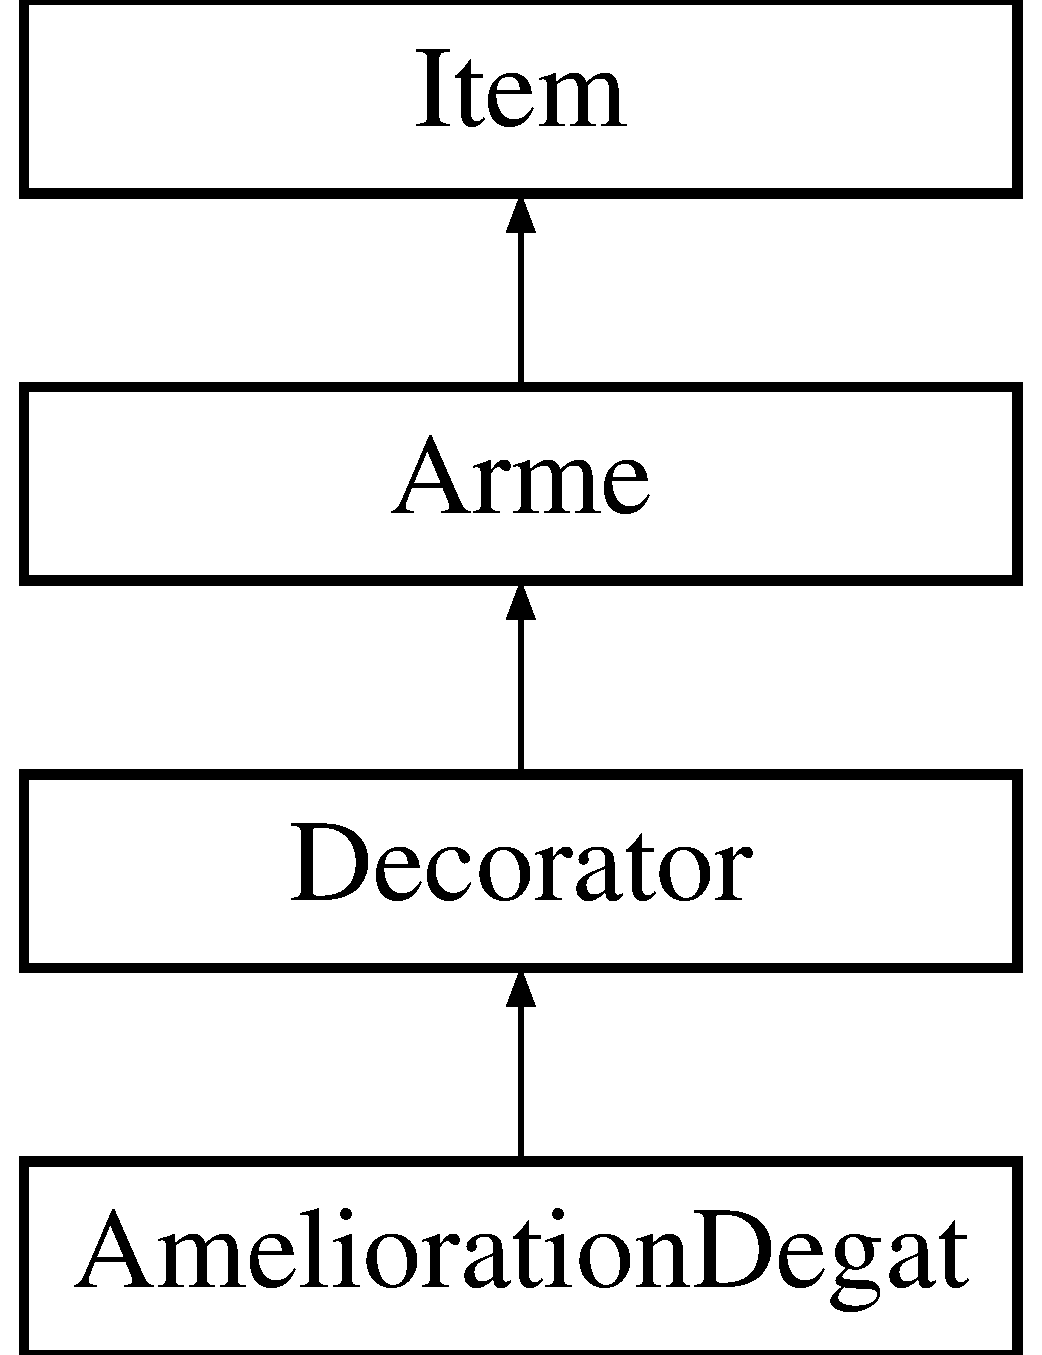
\includegraphics[height=4.000000cm]{classAmeliorationDegat}
\end{center}
\end{figure}
\subsection*{Fonctions membres publiques}
\begin{DoxyCompactItemize}
\item 
\hyperlink{classAmeliorationDegat_a5f3d3c953f2487391872a978eeafb03f}{Amelioration\-Degat} (\hyperlink{classArme}{Arme} $\ast$arme)
\begin{DoxyCompactList}\small\item\em Décorateur de dégats modifiant les dégâts de l'arme. \end{DoxyCompactList}\end{DoxyCompactItemize}
\subsection*{Membres hérités additionnels}


\subsection{Documentation des constructeurs et destructeur}
\hypertarget{classAmeliorationDegat_a5f3d3c953f2487391872a978eeafb03f}{\index{Amelioration\-Degat@{Amelioration\-Degat}!Amelioration\-Degat@{Amelioration\-Degat}}
\index{Amelioration\-Degat@{Amelioration\-Degat}!AmeliorationDegat@{Amelioration\-Degat}}
\subsubsection[{Amelioration\-Degat}]{\setlength{\rightskip}{0pt plus 5cm}Amelioration\-Degat\-::\-Amelioration\-Degat (
\begin{DoxyParamCaption}
\item[{{\bf Arme} $\ast$}]{arme}
\end{DoxyParamCaption}
)}}\label{classAmeliorationDegat_a5f3d3c953f2487391872a978eeafb03f}


Décorateur de dégats modifiant les dégâts de l'arme. 


\begin{DoxyParams}{Paramètres}
{\em arme} & l'arme à décorer. \\
\hline
\end{DoxyParams}


La documentation de cette classe a été générée à partir des fichiers suivants \-:\begin{DoxyCompactItemize}
\item 
Armes.\-hpp\item 
Armes.\-cpp\end{DoxyCompactItemize}

\hypertarget{classAmeliorationPrecision}{\section{Référence de la classe Amelioration\-Precision}
\label{classAmeliorationPrecision}\index{Amelioration\-Precision@{Amelioration\-Precision}}
}
Graphe d'héritage de Amelioration\-Precision\-:\begin{figure}[H]
\begin{center}
\leavevmode
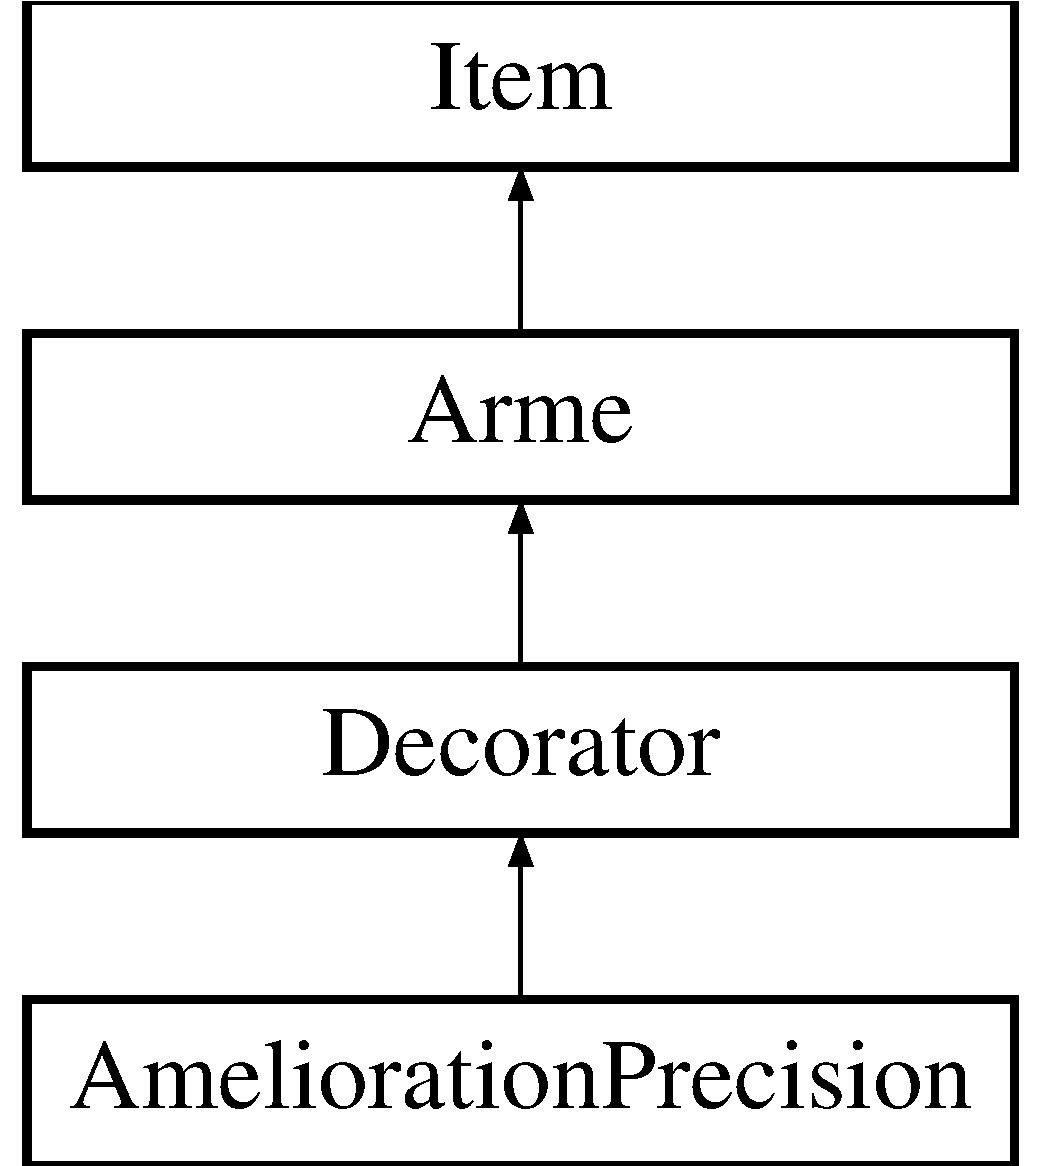
\includegraphics[height=4.000000cm]{classAmeliorationPrecision}
\end{center}
\end{figure}
\subsection*{Fonctions membres publiques}
\begin{DoxyCompactItemize}
\item 
\hyperlink{classAmeliorationPrecision_a32381e99adbda0cba1e8e6568a0a7954}{Amelioration\-Precision} (\hyperlink{classArme}{Arme} $\ast$arme)
\begin{DoxyCompactList}\small\item\em Décorateur de precision modifiant la precision de l'arme. \end{DoxyCompactList}\end{DoxyCompactItemize}
\subsection*{Membres hérités additionnels}


\subsection{Documentation des constructeurs et destructeur}
\hypertarget{classAmeliorationPrecision_a32381e99adbda0cba1e8e6568a0a7954}{\index{Amelioration\-Precision@{Amelioration\-Precision}!Amelioration\-Precision@{Amelioration\-Precision}}
\index{Amelioration\-Precision@{Amelioration\-Precision}!AmeliorationPrecision@{Amelioration\-Precision}}
\subsubsection[{Amelioration\-Precision}]{\setlength{\rightskip}{0pt plus 5cm}Amelioration\-Precision\-::\-Amelioration\-Precision (
\begin{DoxyParamCaption}
\item[{{\bf Arme} $\ast$}]{arme}
\end{DoxyParamCaption}
)}}\label{classAmeliorationPrecision_a32381e99adbda0cba1e8e6568a0a7954}


Décorateur de precision modifiant la precision de l'arme. 


\begin{DoxyParams}{Paramètres}
{\em arme} & l'arme à décorer. \\
\hline
\end{DoxyParams}


La documentation de cette classe a été générée à partir des fichiers suivants \-:\begin{DoxyCompactItemize}
\item 
Armes.\-hpp\item 
Armes.\-cpp\end{DoxyCompactItemize}

\hypertarget{classArme}{\section{Référence de la classe Arme}
\label{classArme}\index{Arme@{Arme}}
}
Graphe d'héritage de Arme\-:\begin{figure}[H]
\begin{center}
\leavevmode
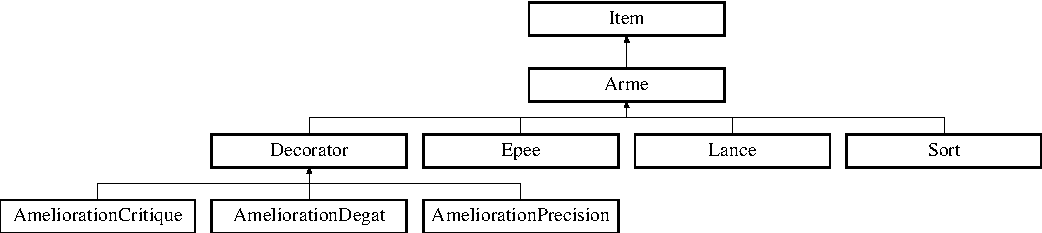
\includegraphics[height=3.132867cm]{classArme}
\end{center}
\end{figure}
\subsection*{Fonctions membres publiques}
\begin{DoxyCompactItemize}
\item 
\hyperlink{classArme_ac0d1cd3296095d25bb2d2f3f50b9f659}{Arme} (std\-::string nom\-Arme, int type, int puissance, int precision, int critique, bool est\-Magique, int prix)
\begin{DoxyCompactList}\small\item\em Le constructeur de l'arme. Constructeur de l'arme instanciant toutes ses caractéristiques. \end{DoxyCompactList}\item 
\hypertarget{classArme_a78288a7d593b4a494f6020f30c5c2383}{virtual \hyperlink{classArme_a78288a7d593b4a494f6020f30c5c2383}{$\sim$\-Arme} ()=0}\label{classArme_a78288a7d593b4a494f6020f30c5c2383}

\begin{DoxyCompactList}\small\item\em Le destructeur de l'arme. \end{DoxyCompactList}\item 
\hypertarget{classArme_a27433c557757a45b7a129bd8e08f6427}{int \hyperlink{classArme_a27433c557757a45b7a129bd8e08f6427}{get\-Type} ()}\label{classArme_a27433c557757a45b7a129bd8e08f6427}

\begin{DoxyCompactList}\small\item\em Le getter du type. \end{DoxyCompactList}\item 
\hypertarget{classArme_a06ced3532b0e60cc900674a94c0cf29b}{int \hyperlink{classArme_a06ced3532b0e60cc900674a94c0cf29b}{get\-Degat} ()}\label{classArme_a06ced3532b0e60cc900674a94c0cf29b}

\begin{DoxyCompactList}\small\item\em Le getter de la puissance. \end{DoxyCompactList}\item 
\hypertarget{classArme_a17e1484872db400cb4c609fa948d1e8a}{int \hyperlink{classArme_a17e1484872db400cb4c609fa948d1e8a}{get\-Precision} ()}\label{classArme_a17e1484872db400cb4c609fa948d1e8a}

\begin{DoxyCompactList}\small\item\em Le getter de la precision. \end{DoxyCompactList}\item 
\hypertarget{classArme_ae228795835d752d3e9dbb1d1c1a167d2}{int \hyperlink{classArme_ae228795835d752d3e9dbb1d1c1a167d2}{get\-Critique} ()}\label{classArme_ae228795835d752d3e9dbb1d1c1a167d2}

\begin{DoxyCompactList}\small\item\em Le getter du pourcentage de critique. \end{DoxyCompactList}\item 
\hypertarget{classArme_a8a869ed0c784eb1c3a1bf3cce5795cc4}{int \hyperlink{classArme_a8a869ed0c784eb1c3a1bf3cce5795cc4}{get\-Prix} ()}\label{classArme_a8a869ed0c784eb1c3a1bf3cce5795cc4}

\begin{DoxyCompactList}\small\item\em Le getter du prix de l'arme. \end{DoxyCompactList}\item 
\hypertarget{classArme_a0a33412d430f095cd0f1670f8e578286}{bool \hyperlink{classArme_a0a33412d430f095cd0f1670f8e578286}{get\-Est\-Magique} ()}\label{classArme_a0a33412d430f095cd0f1670f8e578286}

\begin{DoxyCompactList}\small\item\em Le getter de l'atribut magique ou non. \end{DoxyCompactList}\item 
\hypertarget{classArme_a16daef8f9c593be587010a6daf2b8c88}{void \hyperlink{classArme_a16daef8f9c593be587010a6daf2b8c88}{afficher} ()}\label{classArme_a16daef8f9c593be587010a6daf2b8c88}

\begin{DoxyCompactList}\small\item\em Procédure d'afficahge de l'arme. \end{DoxyCompactList}\item 
void \hyperlink{classArme_ad6704d25feb838154e846c223e041654}{mod\-Nom\-Item} (std\-::string s)
\begin{DoxyCompactList}\small\item\em Modificateur du nom de l'arme. recoit un atribut en paramètre et le met à la suite du nom de l'arme. \end{DoxyCompactList}\item 
void \hyperlink{classArme_aed6c105d30b9ca273035933df2149877}{mod\-Degat} (int a)
\begin{DoxyCompactList}\small\item\em Modificateur de la puissance de l'arme. \end{DoxyCompactList}\item 
void \hyperlink{classArme_a1421ea487a74a824825a93ff15fcbc9d}{mod\-Precision} (int a)
\begin{DoxyCompactList}\small\item\em Modificateur de la precision de l'arme. \end{DoxyCompactList}\item 
void \hyperlink{classArme_a19aa993baf29e53d68e9c55a69025647}{mod\-Critique} (int a)
\begin{DoxyCompactList}\small\item\em Modificateur du pourcentage de critique de l'arme. \end{DoxyCompactList}\end{DoxyCompactItemize}
\subsection*{Attributs protégés}
\begin{DoxyCompactItemize}
\item 
\hypertarget{classArme_a65ba4321c1b097e987a53ed226c4d221}{int {\bfseries type}}\label{classArme_a65ba4321c1b097e987a53ed226c4d221}

\item 
\hypertarget{classArme_a453a2dbaee93971b7ef2bc86739d74e6}{int {\bfseries puissance}}\label{classArme_a453a2dbaee93971b7ef2bc86739d74e6}

\item 
\hypertarget{classArme_a02f45a4001a6ff5af7f7063cc313a6fc}{int {\bfseries precision}}\label{classArme_a02f45a4001a6ff5af7f7063cc313a6fc}

\item 
\hypertarget{classArme_a1399f86fa3aaf69efc334dd7f31d9e5b}{int {\bfseries critique}}\label{classArme_a1399f86fa3aaf69efc334dd7f31d9e5b}

\item 
\hypertarget{classArme_a01d9439024fe325dfd42f3834e553bd1}{bool {\bfseries est\-Magique}}\label{classArme_a01d9439024fe325dfd42f3834e553bd1}

\item 
\hypertarget{classArme_aa805a81304861723d0c11f50e4d15ddf}{int {\bfseries prix}}\label{classArme_aa805a81304861723d0c11f50e4d15ddf}

\end{DoxyCompactItemize}


\subsection{Documentation des constructeurs et destructeur}
\hypertarget{classArme_ac0d1cd3296095d25bb2d2f3f50b9f659}{\index{Arme@{Arme}!Arme@{Arme}}
\index{Arme@{Arme}!Arme@{Arme}}
\subsubsection[{Arme}]{\setlength{\rightskip}{0pt plus 5cm}Arme\-::\-Arme (
\begin{DoxyParamCaption}
\item[{std\-::string}]{nom\-Arme, }
\item[{int}]{type, }
\item[{int}]{puissance, }
\item[{int}]{precision, }
\item[{int}]{critique, }
\item[{bool}]{est\-Magique, }
\item[{int}]{prix}
\end{DoxyParamCaption}
)}}\label{classArme_ac0d1cd3296095d25bb2d2f3f50b9f659}


Le constructeur de l'arme. Constructeur de l'arme instanciant toutes ses caractéristiques. 


\begin{DoxyParams}{Paramètres}
{\em nom\-Arme} & Le nom de l'arme. \\
\hline
{\em type} & I\-D du type de l'arme. \\
\hline
{\em puissance} & La puissance de l'arme. \\
\hline
{\em precision} & La precision de l'arme. \\
\hline
{\em critique} & Son pourcentage de critique. \\
\hline
{\em est\-Magique} & Si oui ou non elle est magique. \\
\hline
{\em prix} & Le prix de base de l'arme. \\
\hline
\end{DoxyParams}


\subsection{Documentation des fonctions membres}
\hypertarget{classArme_a19aa993baf29e53d68e9c55a69025647}{\index{Arme@{Arme}!mod\-Critique@{mod\-Critique}}
\index{mod\-Critique@{mod\-Critique}!Arme@{Arme}}
\subsubsection[{mod\-Critique}]{\setlength{\rightskip}{0pt plus 5cm}void Arme\-::mod\-Critique (
\begin{DoxyParamCaption}
\item[{int}]{a}
\end{DoxyParamCaption}
)}}\label{classArme_a19aa993baf29e53d68e9c55a69025647}


Modificateur du pourcentage de critique de l'arme. 


\begin{DoxyParams}{Paramètres}
{\em a} & Le pourcentage de critique à concaténer. \\
\hline
\end{DoxyParams}
\hypertarget{classArme_aed6c105d30b9ca273035933df2149877}{\index{Arme@{Arme}!mod\-Degat@{mod\-Degat}}
\index{mod\-Degat@{mod\-Degat}!Arme@{Arme}}
\subsubsection[{mod\-Degat}]{\setlength{\rightskip}{0pt plus 5cm}void Arme\-::mod\-Degat (
\begin{DoxyParamCaption}
\item[{int}]{a}
\end{DoxyParamCaption}
)}}\label{classArme_aed6c105d30b9ca273035933df2149877}


Modificateur de la puissance de l'arme. 


\begin{DoxyParams}{Paramètres}
{\em a} & La puissance à concaténer. \\
\hline
\end{DoxyParams}
\hypertarget{classArme_ad6704d25feb838154e846c223e041654}{\index{Arme@{Arme}!mod\-Nom\-Item@{mod\-Nom\-Item}}
\index{mod\-Nom\-Item@{mod\-Nom\-Item}!Arme@{Arme}}
\subsubsection[{mod\-Nom\-Item}]{\setlength{\rightskip}{0pt plus 5cm}void Arme\-::mod\-Nom\-Item (
\begin{DoxyParamCaption}
\item[{std\-::string}]{s}
\end{DoxyParamCaption}
)}}\label{classArme_ad6704d25feb838154e846c223e041654}


Modificateur du nom de l'arme. recoit un atribut en paramètre et le met à la suite du nom de l'arme. 


\begin{DoxyParams}{Paramètres}
{\em s} & Le mot à metre à la suite de l'arme. \\
\hline
\end{DoxyParams}
\hypertarget{classArme_a1421ea487a74a824825a93ff15fcbc9d}{\index{Arme@{Arme}!mod\-Precision@{mod\-Precision}}
\index{mod\-Precision@{mod\-Precision}!Arme@{Arme}}
\subsubsection[{mod\-Precision}]{\setlength{\rightskip}{0pt plus 5cm}void Arme\-::mod\-Precision (
\begin{DoxyParamCaption}
\item[{int}]{a}
\end{DoxyParamCaption}
)}}\label{classArme_a1421ea487a74a824825a93ff15fcbc9d}


Modificateur de la precision de l'arme. 


\begin{DoxyParams}{Paramètres}
{\em a} & La precision à concaténer. \\
\hline
\end{DoxyParams}


La documentation de cette classe a été générée à partir des fichiers suivants \-:\begin{DoxyCompactItemize}
\item 
Armes.\-hpp\item 
Armes.\-cpp\end{DoxyCompactItemize}

\hypertarget{classAttaquant}{\section{Référence de la classe Attaquant}
\label{classAttaquant}\index{Attaquant@{Attaquant}}
}
Graphe d'héritage de Attaquant\-:\begin{figure}[H]
\begin{center}
\leavevmode
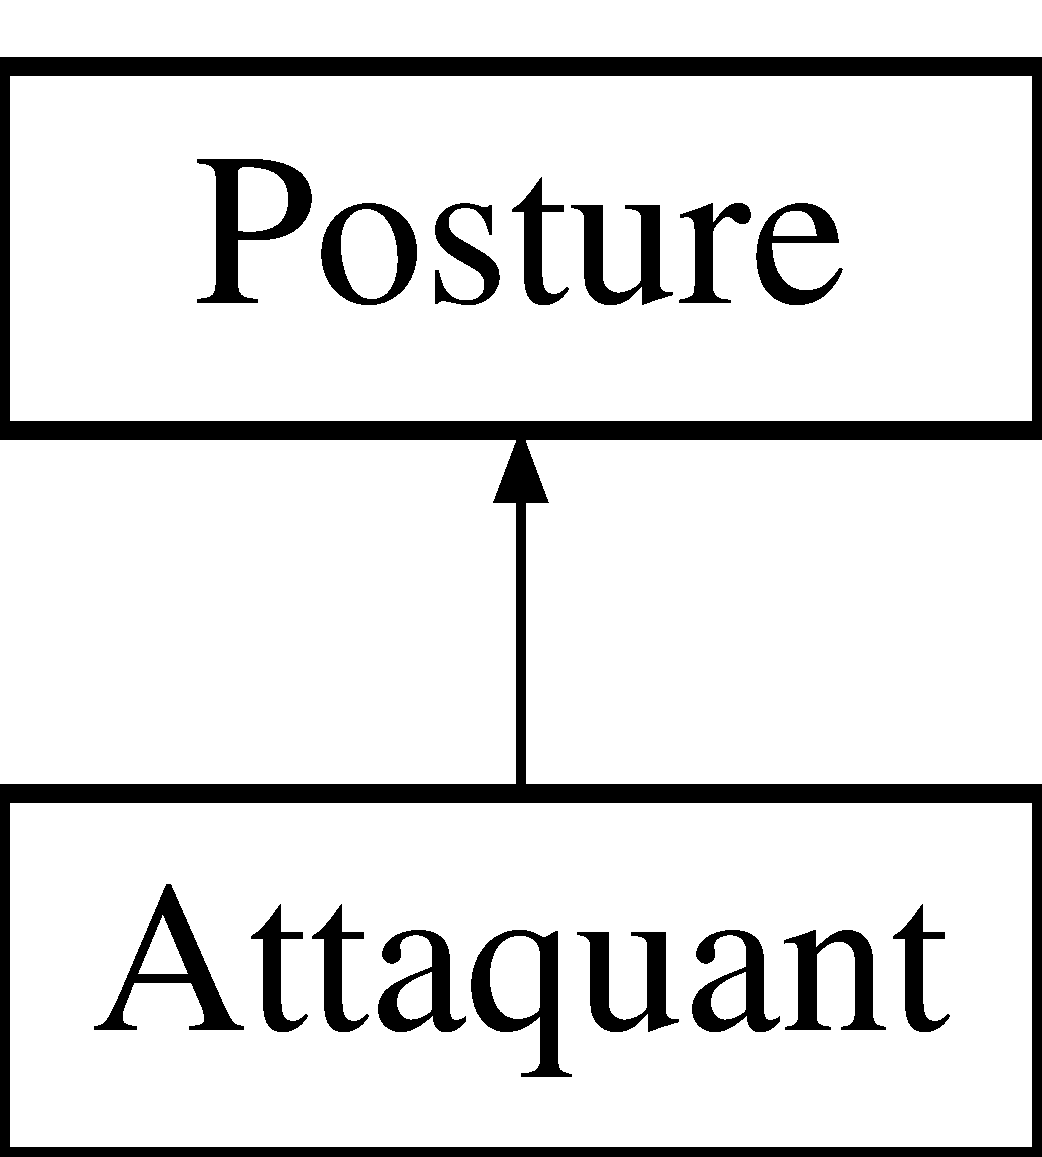
\includegraphics[height=2.000000cm]{classAttaquant}
\end{center}
\end{figure}
\subsection*{Fonctions membres publiques}
\begin{DoxyCompactItemize}
\item 
\hyperlink{classAttaquant_a0bbfef912ef4d22dcbf823ef4447d732}{Attaquant} (int niveau)
\begin{DoxyCompactList}\small\item\em Constructeur de \hyperlink{classAttaquant}{Attaquant} herite de \hyperlink{classPosture}{Posture}. \end{DoxyCompactList}\item 
\hypertarget{classAttaquant_a121cb6666153876071a1dfaf71eef265}{\hyperlink{classAttaquant_a121cb6666153876071a1dfaf71eef265}{$\sim$\-Attaquant} ()}\label{classAttaquant_a121cb6666153876071a1dfaf71eef265}

\begin{DoxyCompactList}\small\item\em Destructeur de \hyperlink{classAttaquant}{Attaquant}. \end{DoxyCompactList}\item 
int \hyperlink{classAttaquant_ad553f75cefdb44bf0703612940d597e4}{attaquer} (int degat)
\begin{DoxyCompactList}\small\item\em comportement de base d'attaque d'\hyperlink{classAttaquant}{Attaquant} \end{DoxyCompactList}\item 
int \hyperlink{classAttaquant_a3aeb7f6ca8b2397dd98bc52219aab836}{subir\-Degat} (int degat)
\begin{DoxyCompactList}\small\item\em comportement de subir\-Degat en \hyperlink{classAttaquant}{Attaquant} \end{DoxyCompactList}\item 
int \hyperlink{classAttaquant_a874dc43af414df3c3c183e452f29a12a}{soigner} (int soin)
\begin{DoxyCompactList}\small\item\em comportement de se soigner en \hyperlink{classAttaquant}{Attaquant} \end{DoxyCompactList}\item 
int \hyperlink{classAttaquant_adda67392faf5ffc39838a03168f1a591}{toucher} (int toucher)
\begin{DoxyCompactList}\small\item\em comportement de toucher en \hyperlink{classAttaquant}{Attaquant} \end{DoxyCompactList}\end{DoxyCompactItemize}
\subsection*{Membres hérités additionnels}


\subsection{Documentation des constructeurs et destructeur}
\hypertarget{classAttaquant_a0bbfef912ef4d22dcbf823ef4447d732}{\index{Attaquant@{Attaquant}!Attaquant@{Attaquant}}
\index{Attaquant@{Attaquant}!Attaquant@{Attaquant}}
\subsubsection[{Attaquant}]{\setlength{\rightskip}{0pt plus 5cm}Attaquant\-::\-Attaquant (
\begin{DoxyParamCaption}
\item[{int}]{niveau}
\end{DoxyParamCaption}
)}}\label{classAttaquant_a0bbfef912ef4d22dcbf823ef4447d732}


Constructeur de \hyperlink{classAttaquant}{Attaquant} herite de \hyperlink{classPosture}{Posture}. 


\begin{DoxyParams}{Paramètres}
{\em niveau} & int le niveau de la posture \\
\hline
\end{DoxyParams}


\subsection{Documentation des fonctions membres}
\hypertarget{classAttaquant_ad553f75cefdb44bf0703612940d597e4}{\index{Attaquant@{Attaquant}!attaquer@{attaquer}}
\index{attaquer@{attaquer}!Attaquant@{Attaquant}}
\subsubsection[{attaquer}]{\setlength{\rightskip}{0pt plus 5cm}int Attaquant\-::attaquer (
\begin{DoxyParamCaption}
\item[{int}]{degat}
\end{DoxyParamCaption}
)\hspace{0.3cm}{\ttfamily [virtual]}}}\label{classAttaquant_ad553f75cefdb44bf0703612940d597e4}


comportement de base d'attaque d'\hyperlink{classAttaquant}{Attaquant} 


\begin{DoxyParams}{Paramètres}
{\em degat} & int les degats de base \\
\hline
\end{DoxyParams}
\begin{DoxyReturn}{Renvoie}
int les degats 
\end{DoxyReturn}


Réimplémentée à partir de \hyperlink{classPosture_ae26355a91999a62fc528a73021e76d1f}{Posture}.

\hypertarget{classAttaquant_a874dc43af414df3c3c183e452f29a12a}{\index{Attaquant@{Attaquant}!soigner@{soigner}}
\index{soigner@{soigner}!Attaquant@{Attaquant}}
\subsubsection[{soigner}]{\setlength{\rightskip}{0pt plus 5cm}int Attaquant\-::soigner (
\begin{DoxyParamCaption}
\item[{int}]{soin}
\end{DoxyParamCaption}
)\hspace{0.3cm}{\ttfamily [virtual]}}}\label{classAttaquant_a874dc43af414df3c3c183e452f29a12a}


comportement de se soigner en \hyperlink{classAttaquant}{Attaquant} 


\begin{DoxyParams}{Paramètres}
{\em soin} & int le nombre de pv soigner de base \\
\hline
\end{DoxyParams}
\begin{DoxyReturn}{Renvoie}
int les le nombre de pv soigner 
\end{DoxyReturn}


Réimplémentée à partir de \hyperlink{classPosture_ab47310e905a5f6de83c945920f7c38b1}{Posture}.

\hypertarget{classAttaquant_a3aeb7f6ca8b2397dd98bc52219aab836}{\index{Attaquant@{Attaquant}!subir\-Degat@{subir\-Degat}}
\index{subir\-Degat@{subir\-Degat}!Attaquant@{Attaquant}}
\subsubsection[{subir\-Degat}]{\setlength{\rightskip}{0pt plus 5cm}int Attaquant\-::subir\-Degat (
\begin{DoxyParamCaption}
\item[{int}]{degat}
\end{DoxyParamCaption}
)\hspace{0.3cm}{\ttfamily [virtual]}}}\label{classAttaquant_a3aeb7f6ca8b2397dd98bc52219aab836}


comportement de subir\-Degat en \hyperlink{classAttaquant}{Attaquant} 


\begin{DoxyParams}{Paramètres}
{\em degat} & int les degats de base \\
\hline
\end{DoxyParams}
\begin{DoxyReturn}{Renvoie}
int les degats 
\end{DoxyReturn}


Réimplémentée à partir de \hyperlink{classPosture_a6c63571b8221847cf0abb1dce0ae1c5f}{Posture}.

\hypertarget{classAttaquant_adda67392faf5ffc39838a03168f1a591}{\index{Attaquant@{Attaquant}!toucher@{toucher}}
\index{toucher@{toucher}!Attaquant@{Attaquant}}
\subsubsection[{toucher}]{\setlength{\rightskip}{0pt plus 5cm}int Attaquant\-::toucher (
\begin{DoxyParamCaption}
\item[{int}]{toucher}
\end{DoxyParamCaption}
)\hspace{0.3cm}{\ttfamily [virtual]}}}\label{classAttaquant_adda67392faf5ffc39838a03168f1a591}


comportement de toucher en \hyperlink{classAttaquant}{Attaquant} 


\begin{DoxyParams}{Paramètres}
{\em degat} & int le pourcentage de chance toucher de base \\
\hline
\end{DoxyParams}
\begin{DoxyReturn}{Renvoie}
int les le pourcentage de chance toucher de base 
\end{DoxyReturn}


Réimplémentée à partir de \hyperlink{classPosture_a0988e92a33908186f74c44b54c1cb6db}{Posture}.



La documentation de cette classe a été générée à partir des fichiers suivants \-:\begin{DoxyCompactItemize}
\item 
Posture.\-hpp\item 
Posture.\-cpp\end{DoxyCompactItemize}

\hypertarget{classBranche}{\section{Référence de la classe Branche}
\label{classBranche}\index{Branche@{Branche}}
}
\subsection*{Fonctions membres publiques}
\begin{DoxyCompactItemize}
\item 
\hyperlink{classBranche_ac81645afe3794d8d3ee7a4726a8668bc}{Branche} (std\-::string nom\-Branche)
\begin{DoxyCompactList}\small\item\em Constructeur de \hyperlink{classBranche}{Branche}. \end{DoxyCompactList}\item 
\hypertarget{classBranche_a67d42a894f0f13f73c0c0bca1dec77cf}{\hyperlink{classBranche_a67d42a894f0f13f73c0c0bca1dec77cf}{$\sim$\-Branche} ()}\label{classBranche_a67d42a894f0f13f73c0c0bca1dec77cf}

\begin{DoxyCompactList}\small\item\em Destructeur de \hyperlink{classBranche}{Branche}. \end{DoxyCompactList}\item 
std\-::string \hyperlink{classBranche_a99127e0e6db3dbce016482a4707a517e}{get\-Citation\-At} (int i)
\begin{DoxyCompactList}\small\item\em donne une citation de la branche \end{DoxyCompactList}\item 
std\-::vector$<$ std\-::string $>$ \hyperlink{classBranche_ad26e7937f3e9521d9891602fc729fe41}{get\-Citations} ()
\begin{DoxyCompactList}\small\item\em getter du vector de citation de la branche \end{DoxyCompactList}\item 
std\-::string \hyperlink{classBranche_a48c9d54e0b68bacb492580e4c3366145}{get\-Nom\-Branche} ()
\begin{DoxyCompactList}\small\item\em getter du nom de la branche \end{DoxyCompactList}\item 
void \hyperlink{classBranche_ac7d895d2d440661c917c8315ac984857}{add\-Citation} (std\-::string citation)
\begin{DoxyCompactList}\small\item\em donne une citation de la branche \end{DoxyCompactList}\item 
void \hyperlink{classBranche_ac1e85c6c41a9e56a146966d468b59462}{vector\-Add6\-String} (std\-::string a, std\-::string b, std\-::string c, std\-::string d, std\-::string e, std\-::string f)
\begin{DoxyCompactList}\small\item\em ajoute six strings au vector de citation de la branche \end{DoxyCompactList}\end{DoxyCompactItemize}


\subsection{Documentation des constructeurs et destructeur}
\hypertarget{classBranche_ac81645afe3794d8d3ee7a4726a8668bc}{\index{Branche@{Branche}!Branche@{Branche}}
\index{Branche@{Branche}!Branche@{Branche}}
\subsubsection[{Branche}]{\setlength{\rightskip}{0pt plus 5cm}Branche\-::\-Branche (
\begin{DoxyParamCaption}
\item[{std\-::string}]{nom\-Branche}
\end{DoxyParamCaption}
)}}\label{classBranche_ac81645afe3794d8d3ee7a4726a8668bc}


Constructeur de \hyperlink{classBranche}{Branche}. 


\begin{DoxyParams}{Paramètres}
{\em nom\-Branche} & string le nom de la branche \\
\hline
\end{DoxyParams}


\subsection{Documentation des fonctions membres}
\hypertarget{classBranche_ac7d895d2d440661c917c8315ac984857}{\index{Branche@{Branche}!add\-Citation@{add\-Citation}}
\index{add\-Citation@{add\-Citation}!Branche@{Branche}}
\subsubsection[{add\-Citation}]{\setlength{\rightskip}{0pt plus 5cm}void Branche\-::add\-Citation (
\begin{DoxyParamCaption}
\item[{std\-::string}]{citation}
\end{DoxyParamCaption}
)}}\label{classBranche_ac7d895d2d440661c917c8315ac984857}


donne une citation de la branche 


\begin{DoxyParams}{Paramètres}
{\em i} & int le numero de la citation \\
\hline
\end{DoxyParams}
\begin{DoxyReturn}{Renvoie}
citation {\itshape string} une citation de la branche 
\end{DoxyReturn}
\hypertarget{classBranche_a99127e0e6db3dbce016482a4707a517e}{\index{Branche@{Branche}!get\-Citation\-At@{get\-Citation\-At}}
\index{get\-Citation\-At@{get\-Citation\-At}!Branche@{Branche}}
\subsubsection[{get\-Citation\-At}]{\setlength{\rightskip}{0pt plus 5cm}std\-::string Branche\-::get\-Citation\-At (
\begin{DoxyParamCaption}
\item[{int}]{i}
\end{DoxyParamCaption}
)}}\label{classBranche_a99127e0e6db3dbce016482a4707a517e}


donne une citation de la branche 


\begin{DoxyParams}{Paramètres}
{\em i} & int le numero de la citation \\
\hline
\end{DoxyParams}
\begin{DoxyReturn}{Renvoie}
citation {\itshape string} une citation de la branche 
\end{DoxyReturn}
\hypertarget{classBranche_ad26e7937f3e9521d9891602fc729fe41}{\index{Branche@{Branche}!get\-Citations@{get\-Citations}}
\index{get\-Citations@{get\-Citations}!Branche@{Branche}}
\subsubsection[{get\-Citations}]{\setlength{\rightskip}{0pt plus 5cm}std\-::vector$<$ std\-::string $>$ Branche\-::get\-Citations (
\begin{DoxyParamCaption}
{}
\end{DoxyParamCaption}
)}}\label{classBranche_ad26e7937f3e9521d9891602fc729fe41}


getter du vector de citation de la branche 

\begin{DoxyReturn}{Renvoie}
citation {\itshape vector$<$std\-::string$>$} 
\end{DoxyReturn}
\hypertarget{classBranche_a48c9d54e0b68bacb492580e4c3366145}{\index{Branche@{Branche}!get\-Nom\-Branche@{get\-Nom\-Branche}}
\index{get\-Nom\-Branche@{get\-Nom\-Branche}!Branche@{Branche}}
\subsubsection[{get\-Nom\-Branche}]{\setlength{\rightskip}{0pt plus 5cm}std\-::string Branche\-::get\-Nom\-Branche (
\begin{DoxyParamCaption}
{}
\end{DoxyParamCaption}
)}}\label{classBranche_a48c9d54e0b68bacb492580e4c3366145}


getter du nom de la branche 

\begin{DoxyReturn}{Renvoie}
nom\-Branche {\itshape std\-::string} 
\end{DoxyReturn}
\hypertarget{classBranche_ac1e85c6c41a9e56a146966d468b59462}{\index{Branche@{Branche}!vector\-Add6\-String@{vector\-Add6\-String}}
\index{vector\-Add6\-String@{vector\-Add6\-String}!Branche@{Branche}}
\subsubsection[{vector\-Add6\-String}]{\setlength{\rightskip}{0pt plus 5cm}void Branche\-::vector\-Add6\-String (
\begin{DoxyParamCaption}
\item[{std\-::string}]{a, }
\item[{std\-::string}]{b, }
\item[{std\-::string}]{c, }
\item[{std\-::string}]{d, }
\item[{std\-::string}]{e, }
\item[{std\-::string}]{f}
\end{DoxyParamCaption}
)}}\label{classBranche_ac1e85c6c41a9e56a146966d468b59462}


ajoute six strings au vector de citation de la branche 


\begin{DoxyParams}{Paramètres}
{\em a} & std\-::string une des six strings ajouter (1er) \\
\hline
{\em b} & std\-::string une des six strings ajouter (2eme) \\
\hline
{\em c} & std\-::string une des six strings ajouter (3eme) \\
\hline
{\em d} & std\-::string une des six strings ajouter (4eme) \\
\hline
{\em e} & std\-::string une des six strings ajouter (5eme) \\
\hline
{\em f} & std\-::string une des six strings ajouter (6eme) \\
\hline
\end{DoxyParams}
\begin{DoxyReturn}{Renvoie}
citation {\itshape string} une citation de la branche 
\end{DoxyReturn}


La documentation de cette classe a été générée à partir des fichiers suivants \-:\begin{DoxyCompactItemize}
\item 
Branche.\-hpp\item 
Branche.\-cpp\end{DoxyCompactItemize}

\hypertarget{classClasse}{\section{Référence de la classe Classe}
\label{classClasse}\index{Classe@{Classe}}
}
Graphe d'héritage de Classe\-:\begin{figure}[H]
\begin{center}
\leavevmode
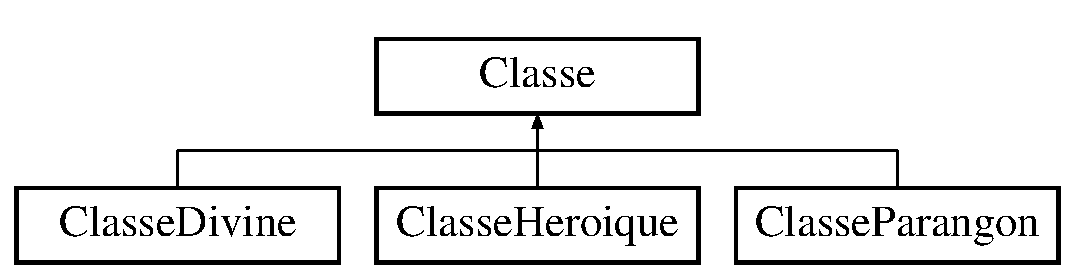
\includegraphics[height=2.000000cm]{classClasse}
\end{center}
\end{figure}
\subsection*{Fonctions membres publiques}
\begin{DoxyCompactItemize}
\item 
\hyperlink{classClasse_a4fca4248505bd69ce2177ef2bdf351e9}{Classe} (std\-::string n\-C, std\-::vector$<$ int $>$ m\-S, \hyperlink{classBranche}{Branche} $\ast$b)
\begin{DoxyCompactList}\small\item\em Constructeur de \hyperlink{classClasse}{Classe} (classe abstaite) \end{DoxyCompactList}\item 
\hypertarget{classClasse_ad98e937acba69b9cfdbf7542c6a1a524}{virtual \hyperlink{classClasse_ad98e937acba69b9cfdbf7542c6a1a524}{$\sim$\-Classe} ()=0}\label{classClasse_ad98e937acba69b9cfdbf7542c6a1a524}

\begin{DoxyCompactList}\small\item\em Destructeur de \hyperlink{classClasse}{Classe}. \end{DoxyCompactList}\item 
std\-::vector$<$ int $>$ \hyperlink{classClasse_a8dfd239db27c6256d2fa36f3e38d66e6}{getmodificateur\-Statistique} ()
\begin{DoxyCompactList}\small\item\em getter de modificateur\-Statistique \end{DoxyCompactList}\item 
std\-::string \hyperlink{classClasse_a3a4ebe85619fe02a302bb8f45b81bc87}{get\-Nom\-Classe} ()
\begin{DoxyCompactList}\small\item\em getter du nom de la classe \end{DoxyCompactList}\item 
std\-::string \hyperlink{classClasse_a01e03d9170bbbf11e3392fe20d41e9a7}{getmodificateur\-Statistique\-String} ()
\begin{DoxyCompactList}\small\item\em retour le vector sous la forme d'une string \end{DoxyCompactList}\item 
\hyperlink{classBranche}{Branche} $\ast$ \hyperlink{classClasse_a1152773b9bd3130aef2fcbde7275021f}{get\-Branche} ()
\begin{DoxyCompactList}\small\item\em getter de la branche \end{DoxyCompactList}\item 
\hypertarget{classClasse_a95c668a4fc6e46680547ec3329729083}{virtual int {\bfseries attaquer} (int degat, int stat\-Attaque)=0}\label{classClasse_a95c668a4fc6e46680547ec3329729083}

\item 
\hypertarget{classClasse_a51971136feda1d0ce4c084ebec33733d}{virtual int {\bfseries mort} (int stat\-Chance, int pv\-Max)=0}\label{classClasse_a51971136feda1d0ce4c084ebec33733d}

\item 
\hypertarget{classClasse_a1d87c06c24ad823261303f8aacac4ab9}{virtual void {\bfseries decheance} (\hyperlink{classPersonnage}{Personnage} $\ast$p)=0}\label{classClasse_a1d87c06c24ad823261303f8aacac4ab9}

\item 
\hypertarget{classClasse_a9cff806b6527767f4bbae6446b7088e7}{virtual bool {\bfseries promotion} (\hyperlink{classPersonnage}{Personnage} $\ast$p, \hyperlink{classClasse}{Classe} $\ast$c)=0}\label{classClasse_a9cff806b6527767f4bbae6446b7088e7}

\end{DoxyCompactItemize}
\subsection*{Attributs protégés}
\begin{DoxyCompactItemize}
\item 
\hypertarget{classClasse_afc4e22634de754a77a7faab629bd55b2}{std\-::string {\bfseries nom\-Classe}}\label{classClasse_afc4e22634de754a77a7faab629bd55b2}

\item 
\hypertarget{classClasse_a4cc191827d081f1fc4ac12b3ff0193e0}{std\-::vector$<$ int $>$ {\bfseries modificateur\-Statistique}}\label{classClasse_a4cc191827d081f1fc4ac12b3ff0193e0}

\item 
\hypertarget{classClasse_aa483c3c732adc751b28d0a4d8e52265a}{\hyperlink{classBranche}{Branche} $\ast$ {\bfseries branche}}\label{classClasse_aa483c3c732adc751b28d0a4d8e52265a}

\end{DoxyCompactItemize}


\subsection{Documentation des constructeurs et destructeur}
\hypertarget{classClasse_a4fca4248505bd69ce2177ef2bdf351e9}{\index{Classe@{Classe}!Classe@{Classe}}
\index{Classe@{Classe}!Classe@{Classe}}
\subsubsection[{Classe}]{\setlength{\rightskip}{0pt plus 5cm}Classe\-::\-Classe (
\begin{DoxyParamCaption}
\item[{std\-::string}]{n\-C, }
\item[{std\-::vector$<$ int $>$}]{m\-S, }
\item[{{\bf Branche} $\ast$}]{b}
\end{DoxyParamCaption}
)}}\label{classClasse_a4fca4248505bd69ce2177ef2bdf351e9}


Constructeur de \hyperlink{classClasse}{Classe} (classe abstaite) 


\begin{DoxyParams}{Paramètres}
{\em n\-C} & std\-::string le nom de la classe \\
\hline
{\em m\-S} & std\-::vector$<$int$>$ les modificateurs de la classe \\
\hline
{\em b} & Branche$\ast$ sa branche \\
\hline
\end{DoxyParams}


\subsection{Documentation des fonctions membres}
\hypertarget{classClasse_a1152773b9bd3130aef2fcbde7275021f}{\index{Classe@{Classe}!get\-Branche@{get\-Branche}}
\index{get\-Branche@{get\-Branche}!Classe@{Classe}}
\subsubsection[{get\-Branche}]{\setlength{\rightskip}{0pt plus 5cm}{\bf Branche} $\ast$ Classe\-::get\-Branche (
\begin{DoxyParamCaption}
{}
\end{DoxyParamCaption}
)}}\label{classClasse_a1152773b9bd3130aef2fcbde7275021f}


getter de la branche 

\begin{DoxyReturn}{Renvoie}
branche Branche$\ast$ la branche de la classe 
\end{DoxyReturn}
\hypertarget{classClasse_a8dfd239db27c6256d2fa36f3e38d66e6}{\index{Classe@{Classe}!getmodificateur\-Statistique@{getmodificateur\-Statistique}}
\index{getmodificateur\-Statistique@{getmodificateur\-Statistique}!Classe@{Classe}}
\subsubsection[{getmodificateur\-Statistique}]{\setlength{\rightskip}{0pt plus 5cm}std\-::vector$<$ int $>$ Classe\-::getmodificateur\-Statistique (
\begin{DoxyParamCaption}
{}
\end{DoxyParamCaption}
)}}\label{classClasse_a8dfd239db27c6256d2fa36f3e38d66e6}


getter de modificateur\-Statistique 

\begin{DoxyReturn}{Renvoie}
modificateur\-Statistique std\-::vector$<$int$>$ le vector de stat 
\end{DoxyReturn}
\hypertarget{classClasse_a01e03d9170bbbf11e3392fe20d41e9a7}{\index{Classe@{Classe}!getmodificateur\-Statistique\-String@{getmodificateur\-Statistique\-String}}
\index{getmodificateur\-Statistique\-String@{getmodificateur\-Statistique\-String}!Classe@{Classe}}
\subsubsection[{getmodificateur\-Statistique\-String}]{\setlength{\rightskip}{0pt plus 5cm}std\-::string Classe\-::getmodificateur\-Statistique\-String (
\begin{DoxyParamCaption}
{}
\end{DoxyParamCaption}
)}}\label{classClasse_a01e03d9170bbbf11e3392fe20d41e9a7}


retour le vector sous la forme d'une string 

\begin{DoxyReturn}{Renvoie}
vector std\-::string 
\end{DoxyReturn}
\hypertarget{classClasse_a3a4ebe85619fe02a302bb8f45b81bc87}{\index{Classe@{Classe}!get\-Nom\-Classe@{get\-Nom\-Classe}}
\index{get\-Nom\-Classe@{get\-Nom\-Classe}!Classe@{Classe}}
\subsubsection[{get\-Nom\-Classe}]{\setlength{\rightskip}{0pt plus 5cm}std\-::string Classe\-::get\-Nom\-Classe (
\begin{DoxyParamCaption}
{}
\end{DoxyParamCaption}
)}}\label{classClasse_a3a4ebe85619fe02a302bb8f45b81bc87}


getter du nom de la classe 

\begin{DoxyReturn}{Renvoie}
modificateur\-Statistique std\-::string le nom de la classe 
\end{DoxyReturn}


La documentation de cette classe a été générée à partir des fichiers suivants \-:\begin{DoxyCompactItemize}
\item 
Classe.\-hpp\item 
Classe.\-cpp\end{DoxyCompactItemize}

\hypertarget{classClasseDivine}{\section{Référence de la classe Classe\-Divine}
\label{classClasseDivine}\index{Classe\-Divine@{Classe\-Divine}}
}
Graphe d'héritage de Classe\-Divine\-:\begin{figure}[H]
\begin{center}
\leavevmode
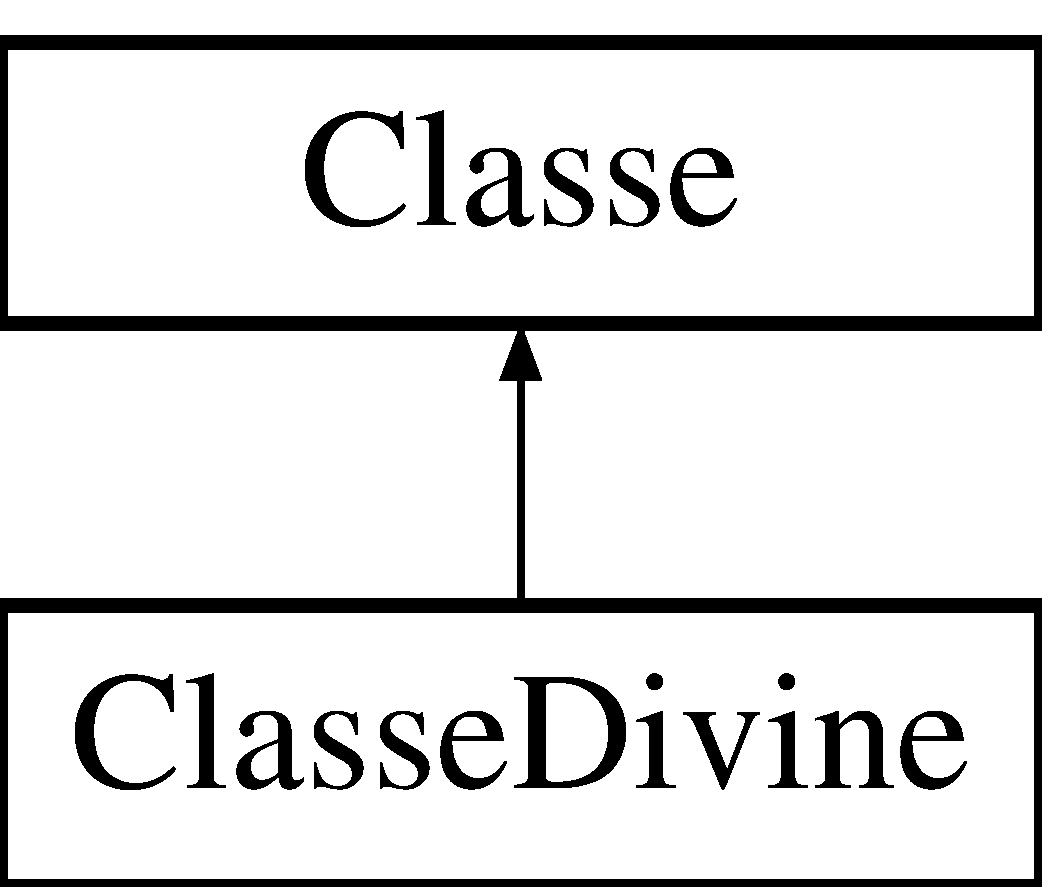
\includegraphics[height=2.000000cm]{classClasseDivine}
\end{center}
\end{figure}
\subsection*{Fonctions membres publiques}
\begin{DoxyCompactItemize}
\item 
\hyperlink{classClasseDivine_a1c6c42d3c8f3d92e6d0ded16fe7b82ad}{Classe\-Divine} (std\-::string n\-C, std\-::vector$<$ int $>$ ms, \hyperlink{classBranche}{Branche} $\ast$b, \hyperlink{classTechnique}{Technique} $\ast$t1, int n\-T1)
\begin{DoxyCompactList}\small\item\em Constructeur de \hyperlink{classClasseDivine}{Classe\-Divine} herite de \hyperlink{classClasse}{Classe}. \end{DoxyCompactList}\item 
\hypertarget{classClasseDivine_abfdf4a1e3c75e2ff45d9a4558b27a003}{\hyperlink{classClasseDivine_abfdf4a1e3c75e2ff45d9a4558b27a003}{$\sim$\-Classe\-Divine} ()}\label{classClasseDivine_abfdf4a1e3c75e2ff45d9a4558b27a003}

\begin{DoxyCompactList}\small\item\em Destructeur de \hyperlink{classClasseDivine}{Classe\-Divine}. \end{DoxyCompactList}\item 
\hyperlink{classTechnique}{Technique} $\ast$ \hyperlink{classClasseDivine_ad5bf8bbab68ba8b0dc5c61f97b0f0190}{get\-Technique1} ()
\begin{DoxyCompactList}\small\item\em getter de la 1er technique \end{DoxyCompactList}\item 
int \hyperlink{classClasseDivine_a6d2e2f72884c04cb90582879665e8dc2}{getniveau\-Technique1} ()
\begin{DoxyCompactList}\small\item\em getter du niveau pour la 1er technique \end{DoxyCompactList}\item 
int \hyperlink{classClasseDivine_a91cef59fd50031801e64ceffa6b979ab}{attaquer} (int degat, int stat\-Attaque)
\begin{DoxyCompactList}\small\item\em methode d'attaque (change en fonction de la classe) \end{DoxyCompactList}\item 
int \hyperlink{classClasseDivine_af8a138f468768c9415325f4090cc24ab}{mort} (int stat\-Chance, int pv\-Max)
\begin{DoxyCompactList}\small\item\em determine si le perso peux regagner miraculeusement des pv(change en fonction de la classe) \end{DoxyCompactList}\item 
void \hyperlink{classClasseDivine_afe770976dc99f0d7b9a7ad53f4523741}{decheance} (\hyperlink{classPersonnage}{Personnage} $\ast$p)
\begin{DoxyCompactList}\small\item\em methode de \char`\"{}transition vers le bas\char`\"{} \end{DoxyCompactList}\item 
bool \hyperlink{classClasseDivine_aa0b67e83394449bf4eb49d2cba44ba19}{promotion} (\hyperlink{classPersonnage}{Personnage} $\ast$p, \hyperlink{classClasse}{Classe} $\ast$c)
\begin{DoxyCompactList}\small\item\em methode de \char`\"{}transition vers le haut\char`\"{} en Divin elle retour T\-O\-U\-J\-O\-U\-R\-S faux \end{DoxyCompactList}\end{DoxyCompactItemize}
\subsection*{Membres hérités additionnels}


\subsection{Documentation des constructeurs et destructeur}
\hypertarget{classClasseDivine_a1c6c42d3c8f3d92e6d0ded16fe7b82ad}{\index{Classe\-Divine@{Classe\-Divine}!Classe\-Divine@{Classe\-Divine}}
\index{Classe\-Divine@{Classe\-Divine}!ClasseDivine@{Classe\-Divine}}
\subsubsection[{Classe\-Divine}]{\setlength{\rightskip}{0pt plus 5cm}Classe\-Divine\-::\-Classe\-Divine (
\begin{DoxyParamCaption}
\item[{std\-::string}]{nc, }
\item[{std\-::vector$<$ int $>$}]{ms, }
\item[{{\bf Branche} $\ast$}]{b, }
\item[{{\bf Technique} $\ast$}]{t1, }
\item[{int}]{n\-T1}
\end{DoxyParamCaption}
)}}\label{classClasseDivine_a1c6c42d3c8f3d92e6d0ded16fe7b82ad}


Constructeur de \hyperlink{classClasseDivine}{Classe\-Divine} herite de \hyperlink{classClasse}{Classe}. 


\begin{DoxyParams}{Paramètres}
{\em n\-C} & std\-::string le nom de la classe \\
\hline
{\em m\-S} & std\-::vector$<$int$>$ les modificateurs de la classe \\
\hline
{\em b} & Branche$\ast$ sa branche \\
\hline
{\em t1} & Technique$\ast$ technique 1 \\
\hline
{\em n\-T1} & int niveau technique 1 \\
\hline
\end{DoxyParams}


\subsection{Documentation des fonctions membres}
\hypertarget{classClasseDivine_a91cef59fd50031801e64ceffa6b979ab}{\index{Classe\-Divine@{Classe\-Divine}!attaquer@{attaquer}}
\index{attaquer@{attaquer}!ClasseDivine@{Classe\-Divine}}
\subsubsection[{attaquer}]{\setlength{\rightskip}{0pt plus 5cm}int Classe\-Divine\-::attaquer (
\begin{DoxyParamCaption}
\item[{int}]{degat, }
\item[{int}]{stat\-Attaque}
\end{DoxyParamCaption}
)\hspace{0.3cm}{\ttfamily [virtual]}}}\label{classClasseDivine_a91cef59fd50031801e64ceffa6b979ab}


methode d'attaque (change en fonction de la classe) 


\begin{DoxyParams}{Paramètres}
{\em degat} & int degat \\
\hline
{\em stat\-Attaque} & int force ou intelligence \\
\hline
\end{DoxyParams}


Implémente \hyperlink{classClasse}{Classe}.

\hypertarget{classClasseDivine_afe770976dc99f0d7b9a7ad53f4523741}{\index{Classe\-Divine@{Classe\-Divine}!decheance@{decheance}}
\index{decheance@{decheance}!ClasseDivine@{Classe\-Divine}}
\subsubsection[{decheance}]{\setlength{\rightskip}{0pt plus 5cm}void Classe\-Divine\-::decheance (
\begin{DoxyParamCaption}
\item[{{\bf Personnage} $\ast$}]{p}
\end{DoxyParamCaption}
)\hspace{0.3cm}{\ttfamily [virtual]}}}\label{classClasseDivine_afe770976dc99f0d7b9a7ad53f4523741}


methode de \char`\"{}transition vers le bas\char`\"{} 


\begin{DoxyParams}{Paramètres}
{\em p} & Personnage$\ast$ le perso dechut \\
\hline
\end{DoxyParams}


Implémente \hyperlink{classClasse}{Classe}.

\hypertarget{classClasseDivine_a6d2e2f72884c04cb90582879665e8dc2}{\index{Classe\-Divine@{Classe\-Divine}!getniveau\-Technique1@{getniveau\-Technique1}}
\index{getniveau\-Technique1@{getniveau\-Technique1}!ClasseDivine@{Classe\-Divine}}
\subsubsection[{getniveau\-Technique1}]{\setlength{\rightskip}{0pt plus 5cm}int Classe\-Divine\-::getniveau\-Technique1 (
\begin{DoxyParamCaption}
{}
\end{DoxyParamCaption}
)}}\label{classClasseDivine_a6d2e2f72884c04cb90582879665e8dc2}


getter du niveau pour la 1er technique 

\begin{DoxyReturn}{Renvoie}
technique $\ast$\-Technique la 1er technique 
\end{DoxyReturn}
\hypertarget{classClasseDivine_ad5bf8bbab68ba8b0dc5c61f97b0f0190}{\index{Classe\-Divine@{Classe\-Divine}!get\-Technique1@{get\-Technique1}}
\index{get\-Technique1@{get\-Technique1}!ClasseDivine@{Classe\-Divine}}
\subsubsection[{get\-Technique1}]{\setlength{\rightskip}{0pt plus 5cm}{\bf Technique} $\ast$ Classe\-Divine\-::get\-Technique1 (
\begin{DoxyParamCaption}
{}
\end{DoxyParamCaption}
)}}\label{classClasseDivine_ad5bf8bbab68ba8b0dc5c61f97b0f0190}


getter de la 1er technique 

\begin{DoxyReturn}{Renvoie}
technique $\ast$\-Technique la 1er technique 
\end{DoxyReturn}
\hypertarget{classClasseDivine_af8a138f468768c9415325f4090cc24ab}{\index{Classe\-Divine@{Classe\-Divine}!mort@{mort}}
\index{mort@{mort}!ClasseDivine@{Classe\-Divine}}
\subsubsection[{mort}]{\setlength{\rightskip}{0pt plus 5cm}int Classe\-Divine\-::mort (
\begin{DoxyParamCaption}
\item[{int}]{stat\-Chance, }
\item[{int}]{pv\-Max}
\end{DoxyParamCaption}
)\hspace{0.3cm}{\ttfamily [virtual]}}}\label{classClasseDivine_af8a138f468768c9415325f4090cc24ab}


determine si le perso peux regagner miraculeusement des pv(change en fonction de la classe) 


\begin{DoxyParams}{Paramètres}
{\em stat\-Chance} & int chance du personnage \\
\hline
{\em pv\-Max} & int les pv\-Max du personnage \\
\hline
\end{DoxyParams}


Implémente \hyperlink{classClasse}{Classe}.

\hypertarget{classClasseDivine_aa0b67e83394449bf4eb49d2cba44ba19}{\index{Classe\-Divine@{Classe\-Divine}!promotion@{promotion}}
\index{promotion@{promotion}!ClasseDivine@{Classe\-Divine}}
\subsubsection[{promotion}]{\setlength{\rightskip}{0pt plus 5cm}bool Classe\-Divine\-::promotion (
\begin{DoxyParamCaption}
\item[{{\bf Personnage} $\ast$}]{p, }
\item[{{\bf Classe} $\ast$}]{c}
\end{DoxyParamCaption}
)\hspace{0.3cm}{\ttfamily [virtual]}}}\label{classClasseDivine_aa0b67e83394449bf4eb49d2cba44ba19}


methode de \char`\"{}transition vers le haut\char`\"{} en Divin elle retour T\-O\-U\-J\-O\-U\-R\-S faux 


\begin{DoxyParams}{Paramètres}
{\em p} & Personnage$\ast$ le perso promu \\
\hline
{\em c} & Classe$\ast$ la nouvelle classe du perso \\
\hline
\end{DoxyParams}
\begin{DoxyReturn}{Renvoie}
bool false resultat constant 
\end{DoxyReturn}


Implémente \hyperlink{classClasse}{Classe}.



La documentation de cette classe a été générée à partir des fichiers suivants \-:\begin{DoxyCompactItemize}
\item 
Classe.\-hpp\item 
Classe.\-cpp\end{DoxyCompactItemize}

\hypertarget{classClasseHeroique}{\section{Référence de la classe Classe\-Heroique}
\label{classClasseHeroique}\index{Classe\-Heroique@{Classe\-Heroique}}
}
Graphe d'héritage de Classe\-Heroique\-:\begin{figure}[H]
\begin{center}
\leavevmode
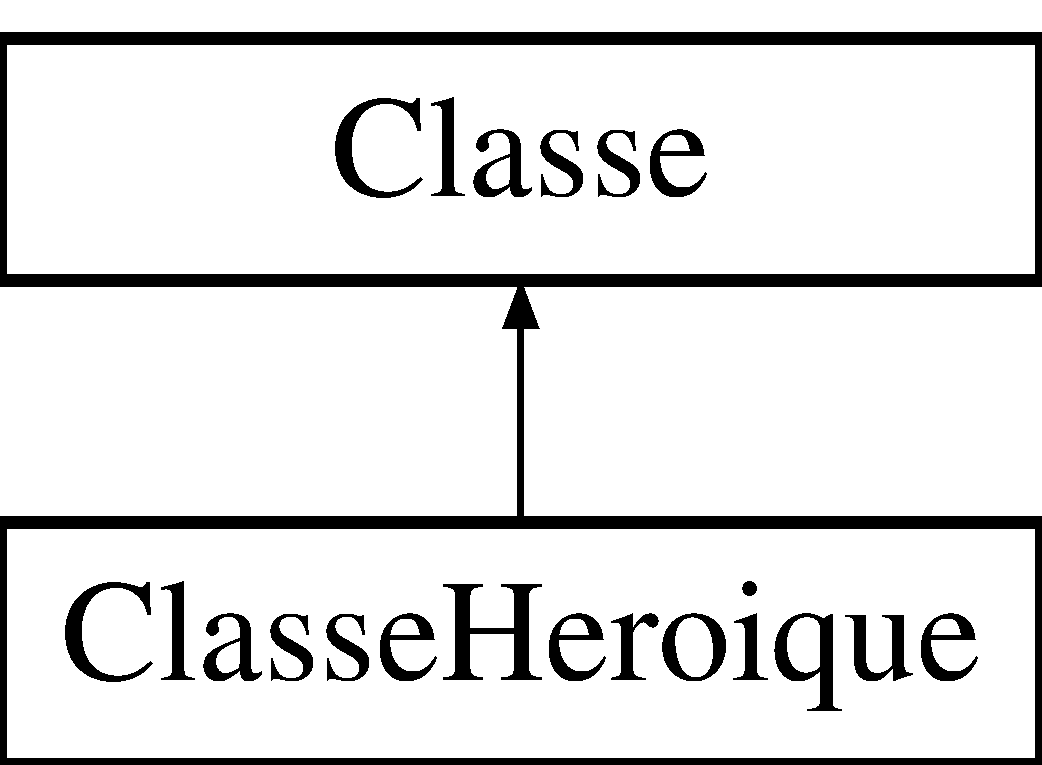
\includegraphics[height=2.000000cm]{classClasseHeroique}
\end{center}
\end{figure}
\subsection*{Fonctions membres publiques}
\begin{DoxyCompactItemize}
\item 
\hyperlink{classClasseHeroique_a94be4fc3d32f2792f8c624ba8ec6911c}{Classe\-Heroique} (std\-::string n\-C, std\-::vector$<$ int $>$ ms, \hyperlink{classBranche}{Branche} $\ast$b, \hyperlink{classTechnique}{Technique} $\ast$t1, \hyperlink{classTechnique}{Technique} $\ast$t2, int n\-T1, int n\-T2)
\begin{DoxyCompactList}\small\item\em Constructeur de \hyperlink{classClasseHeroique}{Classe\-Heroique} herite de \hyperlink{classClasse}{Classe}. \end{DoxyCompactList}\item 
\hypertarget{classClasseHeroique_ad48bcf5829fc43e313376813f32a4170}{\hyperlink{classClasseHeroique_ad48bcf5829fc43e313376813f32a4170}{$\sim$\-Classe\-Heroique} ()}\label{classClasseHeroique_ad48bcf5829fc43e313376813f32a4170}

\begin{DoxyCompactList}\small\item\em Destructeur de \hyperlink{classClasseHeroique}{Classe\-Heroique}. \end{DoxyCompactList}\item 
\hyperlink{classTechnique}{Technique} $\ast$ \hyperlink{classClasseHeroique_a4d08f6ae78e8248c438ab525e7834e17}{get\-Technique1} ()
\begin{DoxyCompactList}\small\item\em getter de la 1er technique \end{DoxyCompactList}\item 
\hyperlink{classTechnique}{Technique} $\ast$ \hyperlink{classClasseHeroique_aade6db9c42e96dc5f34c6263d6391208}{get\-Technique2} ()
\begin{DoxyCompactList}\small\item\em getter de la 2eme technique \end{DoxyCompactList}\item 
int \hyperlink{classClasseHeroique_a19f46bb0d05b35ce775680dcd0d3010b}{getniveau\-Technique1} ()
\begin{DoxyCompactList}\small\item\em getter du niveau pour la 1er technique \end{DoxyCompactList}\item 
int \hyperlink{classClasseHeroique_a61032db45e61f536821ae12e63922f5e}{getniveau\-Technique2} ()
\begin{DoxyCompactList}\small\item\em getter du niveau pour la 2em technique \end{DoxyCompactList}\item 
int \hyperlink{classClasseHeroique_a9811ee389e96597190e99cada8c241e7}{attaquer} (int degat, int stat\-Attaque)
\begin{DoxyCompactList}\small\item\em methode d'attaque (change en fonction de la classe) \end{DoxyCompactList}\item 
int \hyperlink{classClasseHeroique_a5bdbd46d2886a7e71eb1bff34ca5aa6c}{mort} (int stat\-Chance, int pv\-Max)
\begin{DoxyCompactList}\small\item\em determine si le perso peux regagner miraculeusement des pv(change en fonction de la classe) \end{DoxyCompactList}\item 
void \hyperlink{classClasseHeroique_a6aed4bac4cabc6eb09441ea1e2ef7b03}{decheance} (\hyperlink{classPersonnage}{Personnage} $\ast$p)
\begin{DoxyCompactList}\small\item\em methode de \char`\"{}transition vers le bas\char`\"{} \end{DoxyCompactList}\item 
bool \hyperlink{classClasseHeroique_a84e13c85352031c73d5dfbbd691bef30}{promotion} (\hyperlink{classPersonnage}{Personnage} $\ast$p, \hyperlink{classClasse}{Classe} $\ast$c)
\begin{DoxyCompactList}\small\item\em methode de \char`\"{}transition vers le haut\char`\"{} \end{DoxyCompactList}\end{DoxyCompactItemize}
\subsection*{Membres hérités additionnels}


\subsection{Documentation des constructeurs et destructeur}
\hypertarget{classClasseHeroique_a94be4fc3d32f2792f8c624ba8ec6911c}{\index{Classe\-Heroique@{Classe\-Heroique}!Classe\-Heroique@{Classe\-Heroique}}
\index{Classe\-Heroique@{Classe\-Heroique}!ClasseHeroique@{Classe\-Heroique}}
\subsubsection[{Classe\-Heroique}]{\setlength{\rightskip}{0pt plus 5cm}Classe\-Heroique\-::\-Classe\-Heroique (
\begin{DoxyParamCaption}
\item[{std\-::string}]{nc, }
\item[{std\-::vector$<$ int $>$}]{ms, }
\item[{{\bf Branche} $\ast$}]{b, }
\item[{{\bf Technique} $\ast$}]{t1, }
\item[{{\bf Technique} $\ast$}]{t2, }
\item[{int}]{n\-T1, }
\item[{int}]{n\-T2}
\end{DoxyParamCaption}
)}}\label{classClasseHeroique_a94be4fc3d32f2792f8c624ba8ec6911c}


Constructeur de \hyperlink{classClasseHeroique}{Classe\-Heroique} herite de \hyperlink{classClasse}{Classe}. 


\begin{DoxyParams}{Paramètres}
{\em n\-C} & std\-::string le nom de la classe \\
\hline
{\em m\-S} & std\-::vector$<$int$>$ les modificateurs de la classe \\
\hline
{\em b} & Branche$\ast$ sa branche \\
\hline
{\em t1} & Technique$\ast$ technique 1 \\
\hline
{\em t2} & Technique$\ast$ technique 2 \\
\hline
{\em n\-T1} & int niveau technique 1 \\
\hline
{\em n\-T2} & int niveau technique 2 \\
\hline
\end{DoxyParams}


\subsection{Documentation des fonctions membres}
\hypertarget{classClasseHeroique_a9811ee389e96597190e99cada8c241e7}{\index{Classe\-Heroique@{Classe\-Heroique}!attaquer@{attaquer}}
\index{attaquer@{attaquer}!ClasseHeroique@{Classe\-Heroique}}
\subsubsection[{attaquer}]{\setlength{\rightskip}{0pt plus 5cm}int Classe\-Heroique\-::attaquer (
\begin{DoxyParamCaption}
\item[{int}]{degat, }
\item[{int}]{stat\-Attaque}
\end{DoxyParamCaption}
)\hspace{0.3cm}{\ttfamily [virtual]}}}\label{classClasseHeroique_a9811ee389e96597190e99cada8c241e7}


methode d'attaque (change en fonction de la classe) 


\begin{DoxyParams}{Paramètres}
{\em degat} & int degat \\
\hline
{\em stat\-Attaque} & int force ou intelligence \\
\hline
\end{DoxyParams}


Implémente \hyperlink{classClasse}{Classe}.

\hypertarget{classClasseHeroique_a6aed4bac4cabc6eb09441ea1e2ef7b03}{\index{Classe\-Heroique@{Classe\-Heroique}!decheance@{decheance}}
\index{decheance@{decheance}!ClasseHeroique@{Classe\-Heroique}}
\subsubsection[{decheance}]{\setlength{\rightskip}{0pt plus 5cm}void Classe\-Heroique\-::decheance (
\begin{DoxyParamCaption}
\item[{{\bf Personnage} $\ast$}]{p}
\end{DoxyParamCaption}
)\hspace{0.3cm}{\ttfamily [virtual]}}}\label{classClasseHeroique_a6aed4bac4cabc6eb09441ea1e2ef7b03}


methode de \char`\"{}transition vers le bas\char`\"{} 


\begin{DoxyParams}{Paramètres}
{\em p} & Personnage$\ast$ le perso dechut ne doit pas être utiliser \\
\hline
\end{DoxyParams}


Implémente \hyperlink{classClasse}{Classe}.

\hypertarget{classClasseHeroique_a19f46bb0d05b35ce775680dcd0d3010b}{\index{Classe\-Heroique@{Classe\-Heroique}!getniveau\-Technique1@{getniveau\-Technique1}}
\index{getniveau\-Technique1@{getniveau\-Technique1}!ClasseHeroique@{Classe\-Heroique}}
\subsubsection[{getniveau\-Technique1}]{\setlength{\rightskip}{0pt plus 5cm}int Classe\-Heroique\-::getniveau\-Technique1 (
\begin{DoxyParamCaption}
{}
\end{DoxyParamCaption}
)}}\label{classClasseHeroique_a19f46bb0d05b35ce775680dcd0d3010b}


getter du niveau pour la 1er technique 

\begin{DoxyReturn}{Renvoie}
technique $\ast$\-Technique la 1er technique 
\end{DoxyReturn}
\hypertarget{classClasseHeroique_a61032db45e61f536821ae12e63922f5e}{\index{Classe\-Heroique@{Classe\-Heroique}!getniveau\-Technique2@{getniveau\-Technique2}}
\index{getniveau\-Technique2@{getniveau\-Technique2}!ClasseHeroique@{Classe\-Heroique}}
\subsubsection[{getniveau\-Technique2}]{\setlength{\rightskip}{0pt plus 5cm}int Classe\-Heroique\-::getniveau\-Technique2 (
\begin{DoxyParamCaption}
{}
\end{DoxyParamCaption}
)}}\label{classClasseHeroique_a61032db45e61f536821ae12e63922f5e}


getter du niveau pour la 2em technique 

\begin{DoxyReturn}{Renvoie}
technique $\ast$\-Technique la 2eme technique 
\end{DoxyReturn}
\hypertarget{classClasseHeroique_a4d08f6ae78e8248c438ab525e7834e17}{\index{Classe\-Heroique@{Classe\-Heroique}!get\-Technique1@{get\-Technique1}}
\index{get\-Technique1@{get\-Technique1}!ClasseHeroique@{Classe\-Heroique}}
\subsubsection[{get\-Technique1}]{\setlength{\rightskip}{0pt plus 5cm}{\bf Technique} $\ast$ Classe\-Heroique\-::get\-Technique1 (
\begin{DoxyParamCaption}
{}
\end{DoxyParamCaption}
)}}\label{classClasseHeroique_a4d08f6ae78e8248c438ab525e7834e17}


getter de la 1er technique 

\begin{DoxyReturn}{Renvoie}
technique $\ast$\-Technique la 1er technique 
\end{DoxyReturn}
\hypertarget{classClasseHeroique_aade6db9c42e96dc5f34c6263d6391208}{\index{Classe\-Heroique@{Classe\-Heroique}!get\-Technique2@{get\-Technique2}}
\index{get\-Technique2@{get\-Technique2}!ClasseHeroique@{Classe\-Heroique}}
\subsubsection[{get\-Technique2}]{\setlength{\rightskip}{0pt plus 5cm}{\bf Technique} $\ast$ Classe\-Heroique\-::get\-Technique2 (
\begin{DoxyParamCaption}
{}
\end{DoxyParamCaption}
)}}\label{classClasseHeroique_aade6db9c42e96dc5f34c6263d6391208}


getter de la 2eme technique 

\begin{DoxyReturn}{Renvoie}
technique $\ast$\-Technique la 2eme technique 
\end{DoxyReturn}
\hypertarget{classClasseHeroique_a5bdbd46d2886a7e71eb1bff34ca5aa6c}{\index{Classe\-Heroique@{Classe\-Heroique}!mort@{mort}}
\index{mort@{mort}!ClasseHeroique@{Classe\-Heroique}}
\subsubsection[{mort}]{\setlength{\rightskip}{0pt plus 5cm}int Classe\-Heroique\-::mort (
\begin{DoxyParamCaption}
\item[{int}]{stat\-Chance, }
\item[{int}]{pv\-Max}
\end{DoxyParamCaption}
)\hspace{0.3cm}{\ttfamily [virtual]}}}\label{classClasseHeroique_a5bdbd46d2886a7e71eb1bff34ca5aa6c}


determine si le perso peux regagner miraculeusement des pv(change en fonction de la classe) 


\begin{DoxyParams}{Paramètres}
{\em stat\-Chance} & int chance du personnage \\
\hline
{\em pv\-Max} & int les pv\-Max du personnage \\
\hline
\end{DoxyParams}


Implémente \hyperlink{classClasse}{Classe}.

\hypertarget{classClasseHeroique_a84e13c85352031c73d5dfbbd691bef30}{\index{Classe\-Heroique@{Classe\-Heroique}!promotion@{promotion}}
\index{promotion@{promotion}!ClasseHeroique@{Classe\-Heroique}}
\subsubsection[{promotion}]{\setlength{\rightskip}{0pt plus 5cm}bool Classe\-Heroique\-::promotion (
\begin{DoxyParamCaption}
\item[{{\bf Personnage} $\ast$}]{p, }
\item[{{\bf Classe} $\ast$}]{c}
\end{DoxyParamCaption}
)\hspace{0.3cm}{\ttfamily [virtual]}}}\label{classClasseHeroique_a84e13c85352031c73d5dfbbd691bef30}


methode de \char`\"{}transition vers le haut\char`\"{} 


\begin{DoxyParams}{Paramètres}
{\em p} & Personnage$\ast$ le perso promu \\
\hline
{\em c} & Classe$\ast$ la nouvelle classe du perso (doit être Parangon) \\
\hline
\end{DoxyParams}
\begin{DoxyReturn}{Renvoie}
bool true si classe Parangon sinon false 
\end{DoxyReturn}


Implémente \hyperlink{classClasse}{Classe}.



La documentation de cette classe a été générée à partir des fichiers suivants \-:\begin{DoxyCompactItemize}
\item 
Classe.\-hpp\item 
Classe.\-cpp\end{DoxyCompactItemize}

\hypertarget{classClasseParangon}{\section{Référence de la classe Classe\-Parangon}
\label{classClasseParangon}\index{Classe\-Parangon@{Classe\-Parangon}}
}
Graphe d'héritage de Classe\-Parangon\-:\begin{figure}[H]
\begin{center}
\leavevmode
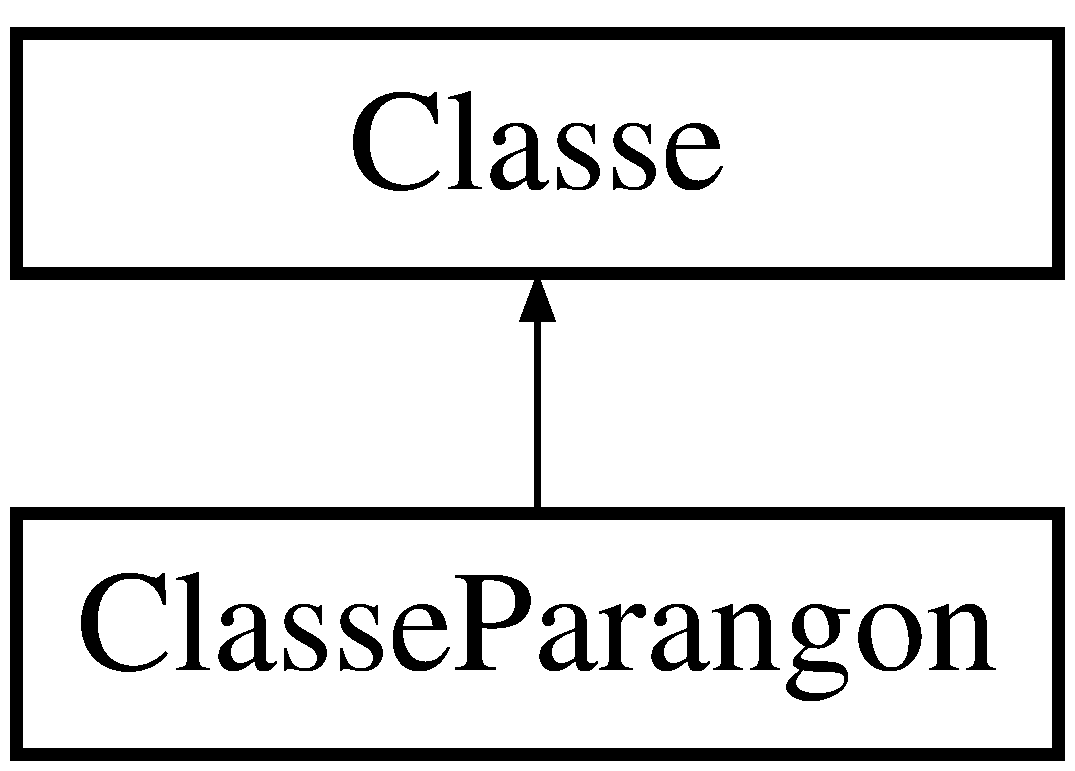
\includegraphics[height=2.000000cm]{classClasseParangon}
\end{center}
\end{figure}
\subsection*{Fonctions membres publiques}
\begin{DoxyCompactItemize}
\item 
\hyperlink{classClasseParangon_a565c2ce61e6902eb9001c04cb9f22ba5}{Classe\-Parangon} (std\-::string n\-C, std\-::vector$<$ int $>$ ms, \hyperlink{classBranche}{Branche} $\ast$b, \hyperlink{classTechnique}{Technique} $\ast$t1, \hyperlink{classTechnique}{Technique} $\ast$t2, int n\-T1, int n\-T2)
\begin{DoxyCompactList}\small\item\em Constructeur de \hyperlink{classClasseParangon}{Classe\-Parangon} herite de \hyperlink{classClasse}{Classe}. \end{DoxyCompactList}\item 
\hypertarget{classClasseParangon_a0bdb8c5ad6c852a02b4d56d6dad7b166}{\hyperlink{classClasseParangon_a0bdb8c5ad6c852a02b4d56d6dad7b166}{$\sim$\-Classe\-Parangon} ()}\label{classClasseParangon_a0bdb8c5ad6c852a02b4d56d6dad7b166}

\begin{DoxyCompactList}\small\item\em Destructeur de \hyperlink{classClasseParangon}{Classe\-Parangon}. \end{DoxyCompactList}\item 
\hyperlink{classTechnique}{Technique} $\ast$ \hyperlink{classClasseParangon_a8999426adeecdc3dcf6b9e25c51d1f57}{get\-Technique1} ()
\begin{DoxyCompactList}\small\item\em getter de la 1er technique \end{DoxyCompactList}\item 
\hyperlink{classTechnique}{Technique} $\ast$ \hyperlink{classClasseParangon_aeac8f67dd301f1474f0064b270b24bde}{get\-Technique2} ()
\begin{DoxyCompactList}\small\item\em getter de la 2eme technique \end{DoxyCompactList}\item 
int \hyperlink{classClasseParangon_abd79d2b688d94086db792d3977fb7203}{getniveau\-Technique1} ()
\begin{DoxyCompactList}\small\item\em getter du niveau pour la 1er technique \end{DoxyCompactList}\item 
int \hyperlink{classClasseParangon_a1964f83ec53a8304300ee9e657e599bc}{getniveau\-Technique2} ()
\begin{DoxyCompactList}\small\item\em getter du niveau pour la 2em technique \end{DoxyCompactList}\item 
int \hyperlink{classClasseParangon_a8c571e469b800a9f7e9e90194a98b7d7}{attaquer} (int degat, int stat\-Attaque)
\begin{DoxyCompactList}\small\item\em methode d'attaque (change en fonction de la classe) \end{DoxyCompactList}\item 
int \hyperlink{classClasseParangon_ac371eb1d2784d30e27f46b375e0fcf39}{mort} (int stat\-Chance, int pv\-Max)
\begin{DoxyCompactList}\small\item\em determine si le perso peux regagner miraculeusement des pv(change en fonction de la classe) \end{DoxyCompactList}\item 
void \hyperlink{classClasseParangon_ac05f4893aa56ca3e9178f6c2f2f4132b}{decheance} (\hyperlink{classPersonnage}{Personnage} $\ast$p)
\begin{DoxyCompactList}\small\item\em methode de \char`\"{}transition vers le bas\char`\"{} \end{DoxyCompactList}\item 
bool \hyperlink{classClasseParangon_abd07f6317ed62a5065fb7aa103387e6b}{promotion} (\hyperlink{classPersonnage}{Personnage} $\ast$p, \hyperlink{classClasse}{Classe} $\ast$c)
\begin{DoxyCompactList}\small\item\em methode de \char`\"{}transition vers le haut\char`\"{} \end{DoxyCompactList}\end{DoxyCompactItemize}
\subsection*{Membres hérités additionnels}


\subsection{Documentation des constructeurs et destructeur}
\hypertarget{classClasseParangon_a565c2ce61e6902eb9001c04cb9f22ba5}{\index{Classe\-Parangon@{Classe\-Parangon}!Classe\-Parangon@{Classe\-Parangon}}
\index{Classe\-Parangon@{Classe\-Parangon}!ClasseParangon@{Classe\-Parangon}}
\subsubsection[{Classe\-Parangon}]{\setlength{\rightskip}{0pt plus 5cm}Classe\-Parangon\-::\-Classe\-Parangon (
\begin{DoxyParamCaption}
\item[{std\-::string}]{nc, }
\item[{std\-::vector$<$ int $>$}]{ms, }
\item[{{\bf Branche} $\ast$}]{b, }
\item[{{\bf Technique} $\ast$}]{t1, }
\item[{{\bf Technique} $\ast$}]{t2, }
\item[{int}]{n\-T1, }
\item[{int}]{n\-T2}
\end{DoxyParamCaption}
)}}\label{classClasseParangon_a565c2ce61e6902eb9001c04cb9f22ba5}


Constructeur de \hyperlink{classClasseParangon}{Classe\-Parangon} herite de \hyperlink{classClasse}{Classe}. 


\begin{DoxyParams}{Paramètres}
{\em n\-C} & std\-::string le nom de la classe \\
\hline
{\em m\-S} & std\-::vector$<$int$>$ les modificateurs de la classe \\
\hline
{\em b} & Branche$\ast$ sa branche \\
\hline
{\em t1} & Technique$\ast$ technique 1 \\
\hline
{\em t2} & Technique$\ast$ technique 2 \\
\hline
{\em n\-T1} & int niveau technique 1 \\
\hline
{\em n\-T2} & int niveau technique 2 \\
\hline
\end{DoxyParams}


\subsection{Documentation des fonctions membres}
\hypertarget{classClasseParangon_a8c571e469b800a9f7e9e90194a98b7d7}{\index{Classe\-Parangon@{Classe\-Parangon}!attaquer@{attaquer}}
\index{attaquer@{attaquer}!ClasseParangon@{Classe\-Parangon}}
\subsubsection[{attaquer}]{\setlength{\rightskip}{0pt plus 5cm}int Classe\-Parangon\-::attaquer (
\begin{DoxyParamCaption}
\item[{int}]{degat, }
\item[{int}]{stat\-Attaque}
\end{DoxyParamCaption}
)\hspace{0.3cm}{\ttfamily [virtual]}}}\label{classClasseParangon_a8c571e469b800a9f7e9e90194a98b7d7}


methode d'attaque (change en fonction de la classe) 


\begin{DoxyParams}{Paramètres}
{\em degat} & int degat \\
\hline
{\em stat\-Attaque} & int force ou intelligence \\
\hline
\end{DoxyParams}


Implémente \hyperlink{classClasse}{Classe}.

\hypertarget{classClasseParangon_ac05f4893aa56ca3e9178f6c2f2f4132b}{\index{Classe\-Parangon@{Classe\-Parangon}!decheance@{decheance}}
\index{decheance@{decheance}!ClasseParangon@{Classe\-Parangon}}
\subsubsection[{decheance}]{\setlength{\rightskip}{0pt plus 5cm}void Classe\-Parangon\-::decheance (
\begin{DoxyParamCaption}
\item[{{\bf Personnage} $\ast$}]{p}
\end{DoxyParamCaption}
)\hspace{0.3cm}{\ttfamily [virtual]}}}\label{classClasseParangon_ac05f4893aa56ca3e9178f6c2f2f4132b}


methode de \char`\"{}transition vers le bas\char`\"{} 


\begin{DoxyParams}{Paramètres}
{\em p} & Personnage$\ast$ le perso dechut \\
\hline
\end{DoxyParams}


Implémente \hyperlink{classClasse}{Classe}.

\hypertarget{classClasseParangon_abd79d2b688d94086db792d3977fb7203}{\index{Classe\-Parangon@{Classe\-Parangon}!getniveau\-Technique1@{getniveau\-Technique1}}
\index{getniveau\-Technique1@{getniveau\-Technique1}!ClasseParangon@{Classe\-Parangon}}
\subsubsection[{getniveau\-Technique1}]{\setlength{\rightskip}{0pt plus 5cm}int Classe\-Parangon\-::getniveau\-Technique1 (
\begin{DoxyParamCaption}
{}
\end{DoxyParamCaption}
)}}\label{classClasseParangon_abd79d2b688d94086db792d3977fb7203}


getter du niveau pour la 1er technique 

\begin{DoxyReturn}{Renvoie}
technique $\ast$\-Technique la 1er technique 
\end{DoxyReturn}
\hypertarget{classClasseParangon_a1964f83ec53a8304300ee9e657e599bc}{\index{Classe\-Parangon@{Classe\-Parangon}!getniveau\-Technique2@{getniveau\-Technique2}}
\index{getniveau\-Technique2@{getniveau\-Technique2}!ClasseParangon@{Classe\-Parangon}}
\subsubsection[{getniveau\-Technique2}]{\setlength{\rightskip}{0pt plus 5cm}int Classe\-Parangon\-::getniveau\-Technique2 (
\begin{DoxyParamCaption}
{}
\end{DoxyParamCaption}
)}}\label{classClasseParangon_a1964f83ec53a8304300ee9e657e599bc}


getter du niveau pour la 2em technique 

\begin{DoxyReturn}{Renvoie}
technique $\ast$\-Technique la 2eme technique 
\end{DoxyReturn}
\hypertarget{classClasseParangon_a8999426adeecdc3dcf6b9e25c51d1f57}{\index{Classe\-Parangon@{Classe\-Parangon}!get\-Technique1@{get\-Technique1}}
\index{get\-Technique1@{get\-Technique1}!ClasseParangon@{Classe\-Parangon}}
\subsubsection[{get\-Technique1}]{\setlength{\rightskip}{0pt plus 5cm}{\bf Technique} $\ast$ Classe\-Parangon\-::get\-Technique1 (
\begin{DoxyParamCaption}
{}
\end{DoxyParamCaption}
)}}\label{classClasseParangon_a8999426adeecdc3dcf6b9e25c51d1f57}


getter de la 1er technique 

\begin{DoxyReturn}{Renvoie}
technique $\ast$\-Technique la 1er technique 
\end{DoxyReturn}
\hypertarget{classClasseParangon_aeac8f67dd301f1474f0064b270b24bde}{\index{Classe\-Parangon@{Classe\-Parangon}!get\-Technique2@{get\-Technique2}}
\index{get\-Technique2@{get\-Technique2}!ClasseParangon@{Classe\-Parangon}}
\subsubsection[{get\-Technique2}]{\setlength{\rightskip}{0pt plus 5cm}{\bf Technique} $\ast$ Classe\-Parangon\-::get\-Technique2 (
\begin{DoxyParamCaption}
{}
\end{DoxyParamCaption}
)}}\label{classClasseParangon_aeac8f67dd301f1474f0064b270b24bde}


getter de la 2eme technique 

\begin{DoxyReturn}{Renvoie}
technique $\ast$\-Technique la 2eme technique 
\end{DoxyReturn}
\hypertarget{classClasseParangon_ac371eb1d2784d30e27f46b375e0fcf39}{\index{Classe\-Parangon@{Classe\-Parangon}!mort@{mort}}
\index{mort@{mort}!ClasseParangon@{Classe\-Parangon}}
\subsubsection[{mort}]{\setlength{\rightskip}{0pt plus 5cm}int Classe\-Parangon\-::mort (
\begin{DoxyParamCaption}
\item[{int}]{stat\-Chance, }
\item[{int}]{pv\-Max}
\end{DoxyParamCaption}
)\hspace{0.3cm}{\ttfamily [virtual]}}}\label{classClasseParangon_ac371eb1d2784d30e27f46b375e0fcf39}


determine si le perso peux regagner miraculeusement des pv(change en fonction de la classe) 


\begin{DoxyParams}{Paramètres}
{\em stat\-Chance} & int chance du personnage \\
\hline
{\em pv\-Max} & int les pv\-Max du personnage \\
\hline
\end{DoxyParams}


Implémente \hyperlink{classClasse}{Classe}.

\hypertarget{classClasseParangon_abd07f6317ed62a5065fb7aa103387e6b}{\index{Classe\-Parangon@{Classe\-Parangon}!promotion@{promotion}}
\index{promotion@{promotion}!ClasseParangon@{Classe\-Parangon}}
\subsubsection[{promotion}]{\setlength{\rightskip}{0pt plus 5cm}bool Classe\-Parangon\-::promotion (
\begin{DoxyParamCaption}
\item[{{\bf Personnage} $\ast$}]{p, }
\item[{{\bf Classe} $\ast$}]{c}
\end{DoxyParamCaption}
)\hspace{0.3cm}{\ttfamily [virtual]}}}\label{classClasseParangon_abd07f6317ed62a5065fb7aa103387e6b}


methode de \char`\"{}transition vers le haut\char`\"{} 


\begin{DoxyParams}{Paramètres}
{\em p} & Personnage$\ast$ le perso promu \\
\hline
{\em c} & Classe$\ast$ la nouvelle classe du perso (doit être Divine) \\
\hline
\end{DoxyParams}
\begin{DoxyReturn}{Renvoie}
bool true si classe divine sinon false 
\end{DoxyReturn}


Implémente \hyperlink{classClasse}{Classe}.



La documentation de cette classe a été générée à partir des fichiers suivants \-:\begin{DoxyCompactItemize}
\item 
Classe.\-hpp\item 
Classe.\-cpp\end{DoxyCompactItemize}

\hypertarget{classCreateurPersonnage}{\section{Référence de la classe Createur\-Personnage}
\label{classCreateurPersonnage}\index{Createur\-Personnage@{Createur\-Personnage}}
}
\subsection*{Fonctions membres publiques}
\begin{DoxyCompactItemize}
\item 
\hypertarget{classCreateurPersonnage_a4ac249d198ea3951c43bef1d3cb392fe}{\hyperlink{classCreateurPersonnage_a4ac249d198ea3951c43bef1d3cb392fe}{Createur\-Personnage} ()}\label{classCreateurPersonnage_a4ac249d198ea3951c43bef1d3cb392fe}

\begin{DoxyCompactList}\small\item\em Constructeur du createur de personnage. \end{DoxyCompactList}\item 
void \hyperlink{classCreateurPersonnage_a37962a1a0e51e54118339119538bf18f}{creation} (\hyperlink{classInstancieur}{Instancieur} inst)
\begin{DoxyCompactList}\small\item\em methode principale du createur de personnage \end{DoxyCompactList}\item 
\hypertarget{classCreateurPersonnage_a7e35c08e904aea2dcaef8c426d0a6559}{bool \hyperlink{classCreateurPersonnage_a7e35c08e904aea2dcaef8c426d0a6559}{confiramation} ()}\label{classCreateurPersonnage_a7e35c08e904aea2dcaef8c426d0a6559}

\begin{DoxyCompactList}\small\item\em methode de confirmation de la creation de personnage \end{DoxyCompactList}\item 
\hypertarget{classCreateurPersonnage_ad19dfee81e9e5a7f9934973bed930d60}{void \hyperlink{classCreateurPersonnage_ad19dfee81e9e5a7f9934973bed930d60}{texte\-Branche} ()}\label{classCreateurPersonnage_ad19dfee81e9e5a7f9934973bed930d60}

\begin{DoxyCompactList}\small\item\em methode d'affichage du texte de selection de branche \end{DoxyCompactList}\item 
void \hyperlink{classCreateurPersonnage_a53a8e0403bd828add3bc1189cc7b4916}{texte\-Classe} ()
\begin{DoxyCompactList}\small\item\em methode d'affichage du texte de selection de classe \end{DoxyCompactList}\item 
void \hyperlink{classCreateurPersonnage_a87026af076710b4ce27aef5c456fb14b}{vector\-Add10\-Int} (std\-::vector$<$ int $>$ \&Vec, int a, int b, int c, int d, int e, int f, int g, int h, int i, int j)
\begin{DoxyCompactList}\small\item\em ajoute dix int au vector de stat \end{DoxyCompactList}\end{DoxyCompactItemize}


\subsection{Documentation des fonctions membres}
\hypertarget{classCreateurPersonnage_a37962a1a0e51e54118339119538bf18f}{\index{Createur\-Personnage@{Createur\-Personnage}!creation@{creation}}
\index{creation@{creation}!CreateurPersonnage@{Createur\-Personnage}}
\subsubsection[{creation}]{\setlength{\rightskip}{0pt plus 5cm}void Createur\-Personnage\-::creation (
\begin{DoxyParamCaption}
\item[{{\bf Instancieur}}]{inst}
\end{DoxyParamCaption}
)}}\label{classCreateurPersonnage_a37962a1a0e51e54118339119538bf18f}


methode principale du createur de personnage 


\begin{DoxyParams}{Paramètres}
{\em inst} & \hyperlink{classInstancieur}{Instancieur} pour avoir les données necessaire a la creation \\
\hline
\end{DoxyParams}
\hypertarget{classCreateurPersonnage_a53a8e0403bd828add3bc1189cc7b4916}{\index{Createur\-Personnage@{Createur\-Personnage}!texte\-Classe@{texte\-Classe}}
\index{texte\-Classe@{texte\-Classe}!CreateurPersonnage@{Createur\-Personnage}}
\subsubsection[{texte\-Classe}]{\setlength{\rightskip}{0pt plus 5cm}void Createur\-Personnage\-::texte\-Classe (
\begin{DoxyParamCaption}
{}
\end{DoxyParamCaption}
)}}\label{classCreateurPersonnage_a53a8e0403bd828add3bc1189cc7b4916}


methode d'affichage du texte de selection de classe 

\begin{DoxyRefDesc}{Bogue}
\item[\hyperlink{bug__bug000001}{Bogue}]pas fini \-:( \end{DoxyRefDesc}
\hypertarget{classCreateurPersonnage_a87026af076710b4ce27aef5c456fb14b}{\index{Createur\-Personnage@{Createur\-Personnage}!vector\-Add10\-Int@{vector\-Add10\-Int}}
\index{vector\-Add10\-Int@{vector\-Add10\-Int}!CreateurPersonnage@{Createur\-Personnage}}
\subsubsection[{vector\-Add10\-Int}]{\setlength{\rightskip}{0pt plus 5cm}void Createur\-Personnage\-::vector\-Add10\-Int (
\begin{DoxyParamCaption}
\item[{std\-::vector$<$ int $>$ \&}]{Vec, }
\item[{int}]{a, }
\item[{int}]{b, }
\item[{int}]{c, }
\item[{int}]{d, }
\item[{int}]{e, }
\item[{int}]{f, }
\item[{int}]{g, }
\item[{int}]{h, }
\item[{int}]{i, }
\item[{int}]{j}
\end{DoxyParamCaption}
)}}\label{classCreateurPersonnage_a87026af076710b4ce27aef5c456fb14b}


ajoute dix int au vector de stat 


\begin{DoxyParams}{Paramètres}
{\em Vec} & std\-::vector$<$int$>$ le vector dans le quel on ajoute \\
\hline
{\em a} & int une des dix int ajouter (1er) \\
\hline
{\em b} & int une des dix int ajouter (2eme) \\
\hline
{\em c} & int une des dix int ajouter (3eme) \\
\hline
{\em d} & int une des dix int ajouter (4eme) \\
\hline
{\em e} & int une des dix int ajouter (5eme) \\
\hline
{\em f} & int une des dix int ajouter (6eme) \\
\hline
{\em g} & int une des dix int ajouter (7eme) \\
\hline
{\em h} & int une des dix int ajouter (8eme) \\
\hline
{\em i} & int une des dix int ajouter (9eme) \\
\hline
{\em j} & int une des dix int ajouter (10eme) \\
\hline
\end{DoxyParams}


La documentation de cette classe a été générée à partir des fichiers suivants \-:\begin{DoxyCompactItemize}
\item 
Createur\-Personnage.\-hpp\item 
Createur\-Personnage.\-cpp\end{DoxyCompactItemize}

\hypertarget{classDecorator}{\section{Référence de la classe Decorator}
\label{classDecorator}\index{Decorator@{Decorator}}
}
Graphe d'héritage de Decorator\-:\begin{figure}[H]
\begin{center}
\leavevmode
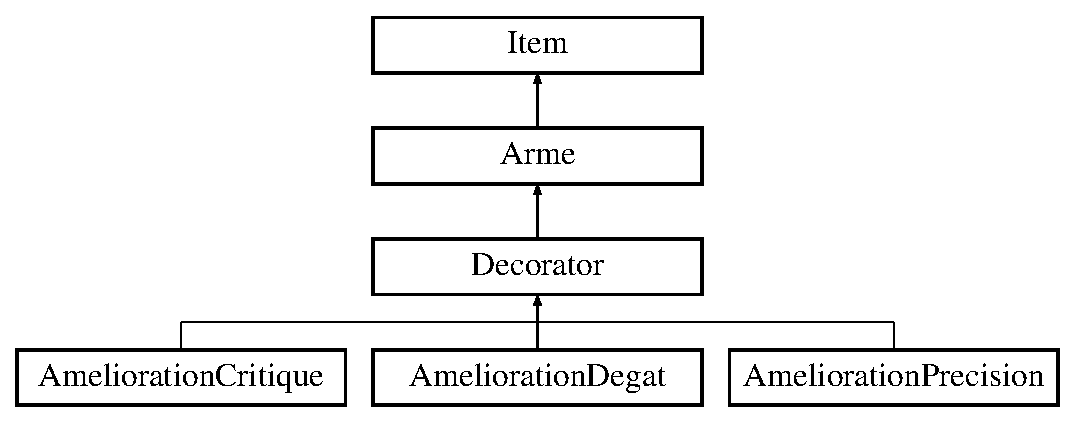
\includegraphics[height=4.000000cm]{classDecorator}
\end{center}
\end{figure}
\subsection*{Fonctions membres publiques}
\begin{DoxyCompactItemize}
\item 
\hyperlink{classDecorator_ac9c52af9f40db0da215bbf782cae1299}{Decorator} (\hyperlink{classArme}{Arme} $\ast$arme)
\begin{DoxyCompactList}\small\item\em Constructeur du décorator copiant la valeur de l'arme en entrée. \end{DoxyCompactList}\end{DoxyCompactItemize}
\subsection*{Attributs protégés}
\begin{DoxyCompactItemize}
\item 
\hypertarget{classDecorator_a9fb863386b1d1bc19037617fe829f2f2}{\hyperlink{classArme}{Arme} $\ast$ {\bfseries arme}}\label{classDecorator_a9fb863386b1d1bc19037617fe829f2f2}

\end{DoxyCompactItemize}


\subsection{Documentation des constructeurs et destructeur}
\hypertarget{classDecorator_ac9c52af9f40db0da215bbf782cae1299}{\index{Decorator@{Decorator}!Decorator@{Decorator}}
\index{Decorator@{Decorator}!Decorator@{Decorator}}
\subsubsection[{Decorator}]{\setlength{\rightskip}{0pt plus 5cm}Decorator\-::\-Decorator (
\begin{DoxyParamCaption}
\item[{{\bf Arme} $\ast$}]{arme}
\end{DoxyParamCaption}
)}}\label{classDecorator_ac9c52af9f40db0da215bbf782cae1299}


Constructeur du décorator copiant la valeur de l'arme en entrée. 


\begin{DoxyParams}{Paramètres}
{\em arme} & l'arme à décorer. \\
\hline
\end{DoxyParams}


La documentation de cette classe a été générée à partir des fichiers suivants \-:\begin{DoxyCompactItemize}
\item 
Armes.\-hpp\item 
Armes.\-cpp\end{DoxyCompactItemize}

\hypertarget{classDefenseur}{\section{Référence de la classe Defenseur}
\label{classDefenseur}\index{Defenseur@{Defenseur}}
}
Graphe d'héritage de Defenseur\-:\begin{figure}[H]
\begin{center}
\leavevmode
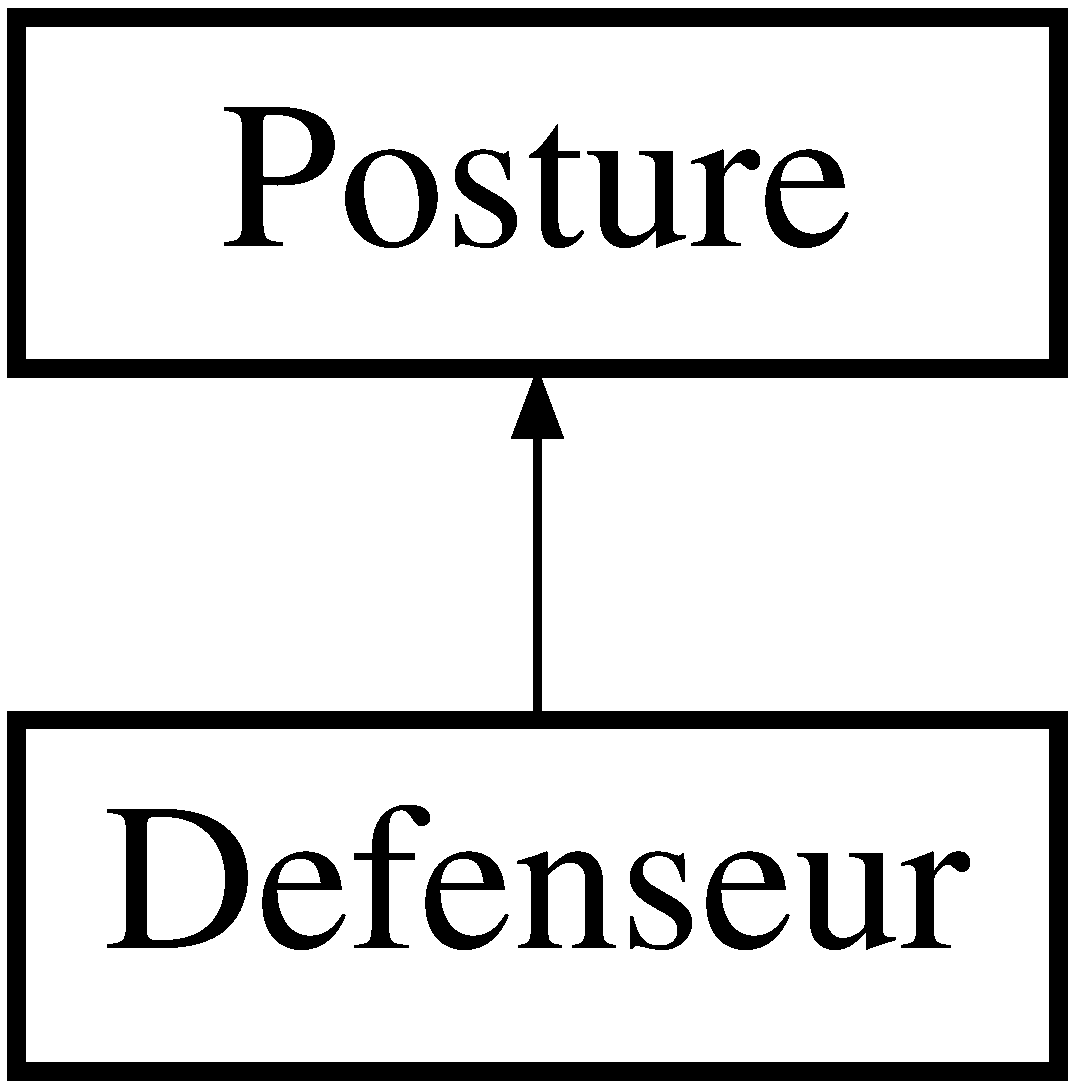
\includegraphics[height=2.000000cm]{classDefenseur}
\end{center}
\end{figure}
\subsection*{Fonctions membres publiques}
\begin{DoxyCompactItemize}
\item 
\hyperlink{classDefenseur_ae49a06db373ffa7a67c77a605db384f4}{Defenseur} (int niveau)
\begin{DoxyCompactList}\small\item\em Constructeur de \hyperlink{classDefenseur}{Defenseur} herite de \hyperlink{classPosture}{Posture}. \end{DoxyCompactList}\item 
\hypertarget{classDefenseur_a85d338156a1df3f8f26b4b17d564d81e}{\hyperlink{classDefenseur_a85d338156a1df3f8f26b4b17d564d81e}{$\sim$\-Defenseur} ()}\label{classDefenseur_a85d338156a1df3f8f26b4b17d564d81e}

\begin{DoxyCompactList}\small\item\em Destructeur de \hyperlink{classDefenseur}{Defenseur}. \end{DoxyCompactList}\item 
int \hyperlink{classDefenseur_a9ec20f4bd6450776be10f4e9b037691d}{attaquer} (int degat)
\begin{DoxyCompactList}\small\item\em comportement d'attaque de \hyperlink{classDefenseur}{Defenseur} \end{DoxyCompactList}\item 
int \hyperlink{classDefenseur_aa8a5e55f036a24005d9fab761d2ca272}{subir\-Degat} (int degat)
\begin{DoxyCompactList}\small\item\em comportement de subir\-Degat en \hyperlink{classDefenseur}{Defenseur} \end{DoxyCompactList}\end{DoxyCompactItemize}
\subsection*{Membres hérités additionnels}


\subsection{Documentation des constructeurs et destructeur}
\hypertarget{classDefenseur_ae49a06db373ffa7a67c77a605db384f4}{\index{Defenseur@{Defenseur}!Defenseur@{Defenseur}}
\index{Defenseur@{Defenseur}!Defenseur@{Defenseur}}
\subsubsection[{Defenseur}]{\setlength{\rightskip}{0pt plus 5cm}Defenseur\-::\-Defenseur (
\begin{DoxyParamCaption}
\item[{int}]{niveau}
\end{DoxyParamCaption}
)}}\label{classDefenseur_ae49a06db373ffa7a67c77a605db384f4}


Constructeur de \hyperlink{classDefenseur}{Defenseur} herite de \hyperlink{classPosture}{Posture}. 


\begin{DoxyParams}{Paramètres}
{\em niveau} & int le niveau de la posture \\
\hline
\end{DoxyParams}


\subsection{Documentation des fonctions membres}
\hypertarget{classDefenseur_a9ec20f4bd6450776be10f4e9b037691d}{\index{Defenseur@{Defenseur}!attaquer@{attaquer}}
\index{attaquer@{attaquer}!Defenseur@{Defenseur}}
\subsubsection[{attaquer}]{\setlength{\rightskip}{0pt plus 5cm}int Defenseur\-::attaquer (
\begin{DoxyParamCaption}
\item[{int}]{degat}
\end{DoxyParamCaption}
)\hspace{0.3cm}{\ttfamily [virtual]}}}\label{classDefenseur_a9ec20f4bd6450776be10f4e9b037691d}


comportement d'attaque de \hyperlink{classDefenseur}{Defenseur} 


\begin{DoxyParams}{Paramètres}
{\em degat} & int les degats de base \\
\hline
\end{DoxyParams}
\begin{DoxyReturn}{Renvoie}
int les degats 
\end{DoxyReturn}


Réimplémentée à partir de \hyperlink{classPosture_ae26355a91999a62fc528a73021e76d1f}{Posture}.

\hypertarget{classDefenseur_aa8a5e55f036a24005d9fab761d2ca272}{\index{Defenseur@{Defenseur}!subir\-Degat@{subir\-Degat}}
\index{subir\-Degat@{subir\-Degat}!Defenseur@{Defenseur}}
\subsubsection[{subir\-Degat}]{\setlength{\rightskip}{0pt plus 5cm}int Defenseur\-::subir\-Degat (
\begin{DoxyParamCaption}
\item[{int}]{degat}
\end{DoxyParamCaption}
)\hspace{0.3cm}{\ttfamily [virtual]}}}\label{classDefenseur_aa8a5e55f036a24005d9fab761d2ca272}


comportement de subir\-Degat en \hyperlink{classDefenseur}{Defenseur} 


\begin{DoxyParams}{Paramètres}
{\em degat} & int les degats de base \\
\hline
\end{DoxyParams}
\begin{DoxyReturn}{Renvoie}
int les degats 
\end{DoxyReturn}


Réimplémentée à partir de \hyperlink{classPosture_a6c63571b8221847cf0abb1dce0ae1c5f}{Posture}.



La documentation de cette classe a été générée à partir des fichiers suivants \-:\begin{DoxyCompactItemize}
\item 
Posture.\-hpp\item 
Posture.\-cpp\end{DoxyCompactItemize}

\hypertarget{classEpee}{\section{Référence de la classe Epee}
\label{classEpee}\index{Epee@{Epee}}
}
Graphe d'héritage de Epee\-:\begin{figure}[H]
\begin{center}
\leavevmode
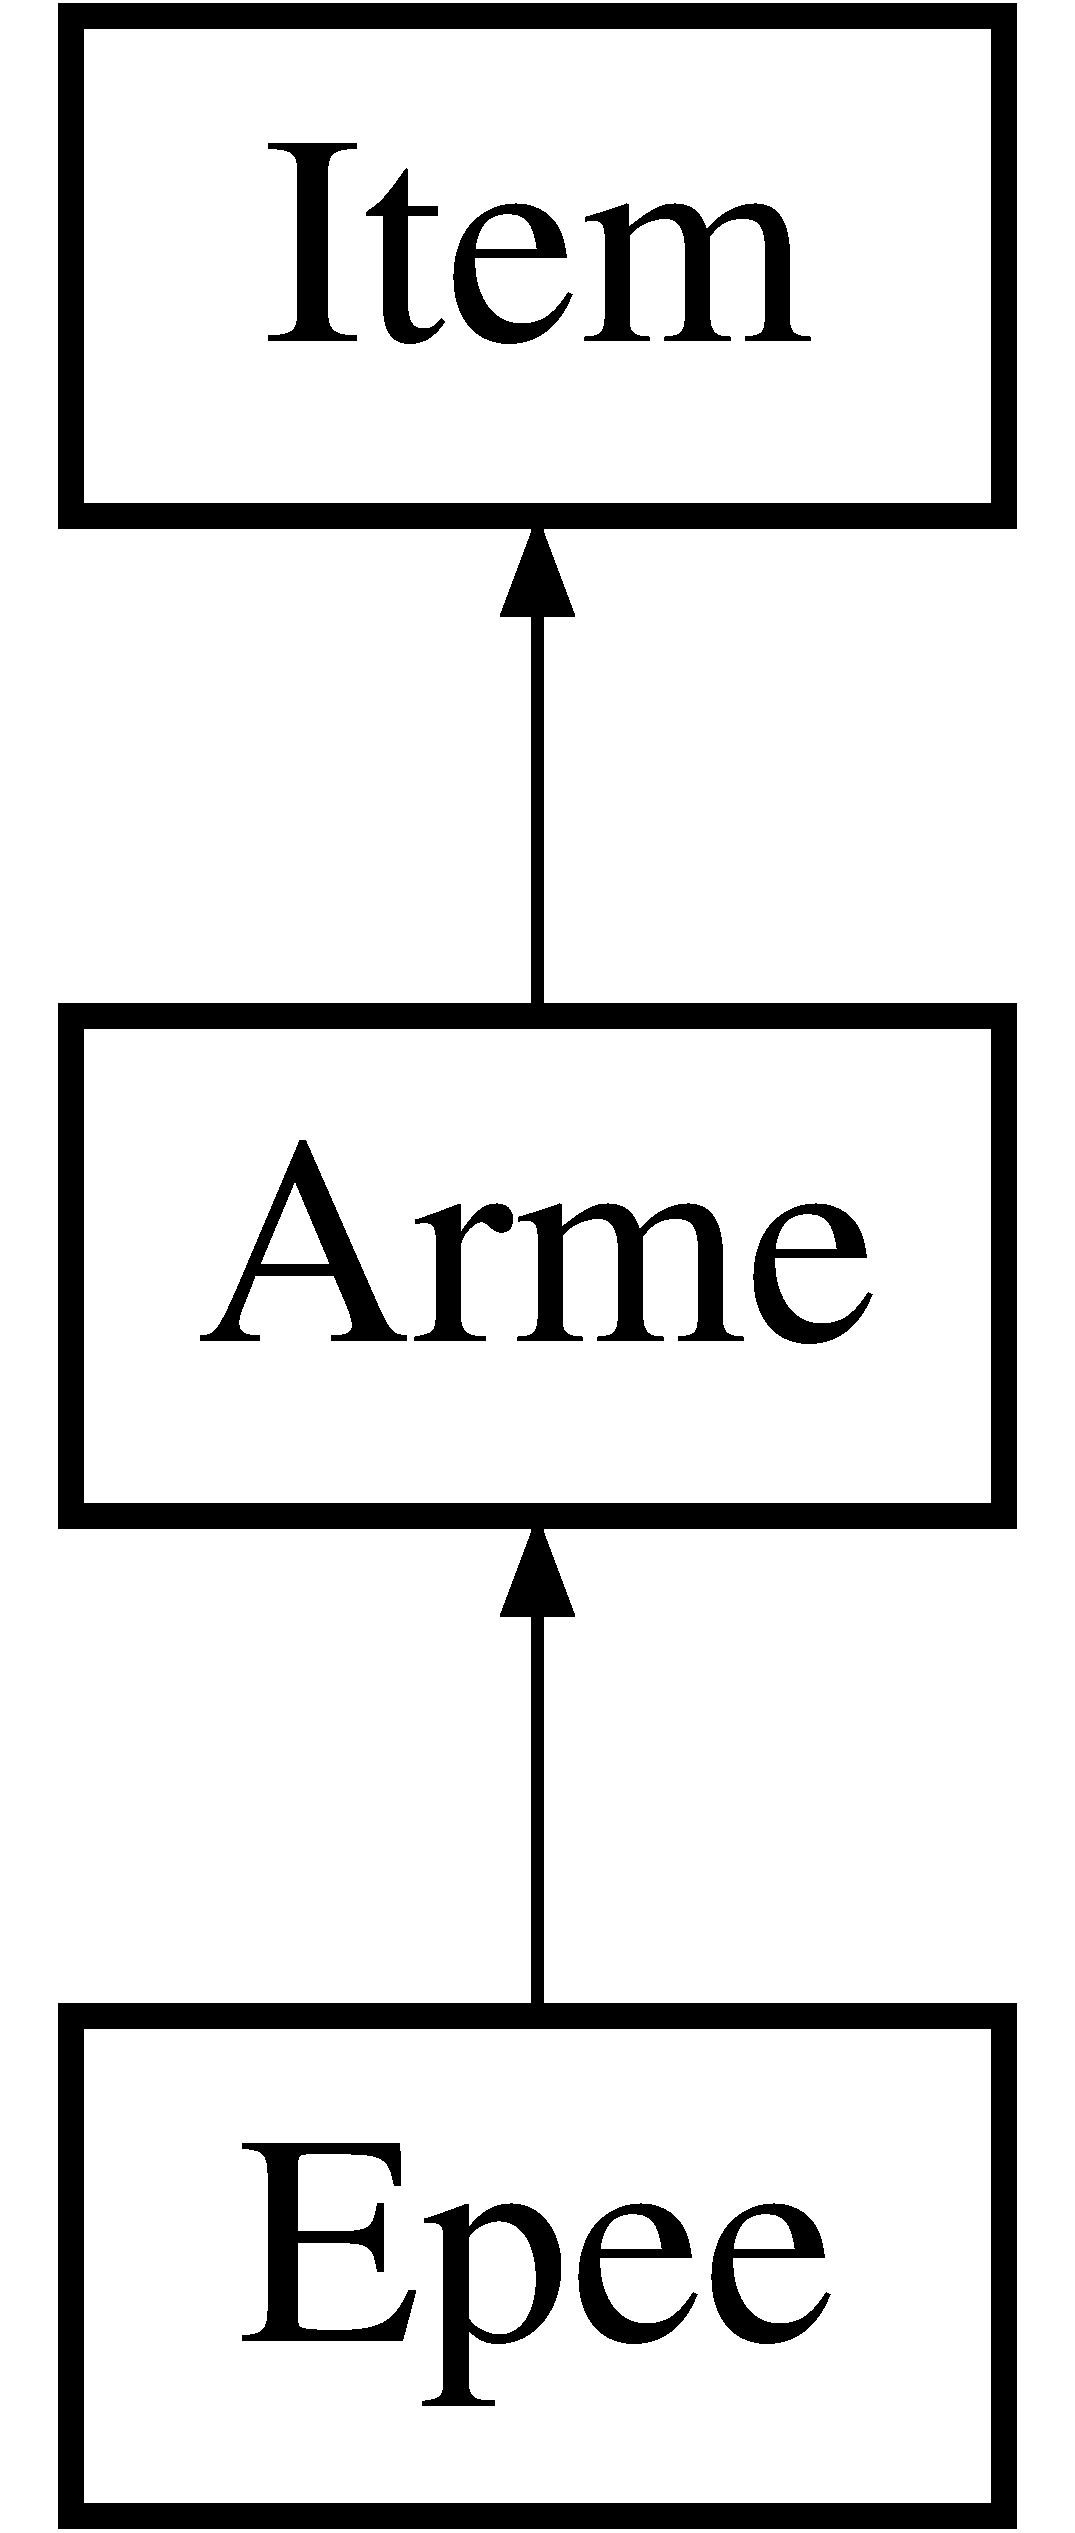
\includegraphics[height=3.000000cm]{classEpee}
\end{center}
\end{figure}
\subsection*{Fonctions membres publiques}
\begin{DoxyCompactItemize}
\item 
\hypertarget{classEpee_a4553a29d6b18c191d6fcf44575a516ae}{\hyperlink{classEpee_a4553a29d6b18c191d6fcf44575a516ae}{Epee} (std\-::string nom\-Arme, int puissance, int precision, int critique, bool est\-Magique, int prix)}\label{classEpee_a4553a29d6b18c191d6fcf44575a516ae}

\begin{DoxyCompactList}\small\item\em Construit une arme de type 0. \end{DoxyCompactList}\end{DoxyCompactItemize}
\subsection*{Membres hérités additionnels}


La documentation de cette classe a été générée à partir des fichiers suivants \-:\begin{DoxyCompactItemize}
\item 
Armes.\-hpp\item 
Armes.\-cpp\end{DoxyCompactItemize}

\hypertarget{classGenerateurPersonnage}{\section{Référence de la classe Generateur\-Personnage}
\label{classGenerateurPersonnage}\index{Generateur\-Personnage@{Generateur\-Personnage}}
}
\subsection*{Fonctions membres publiques}
\begin{DoxyCompactItemize}
\item 
\hypertarget{classGenerateurPersonnage_af62f2f136100c9b47a0791f4e45568ad}{\hyperlink{classPersonnage}{Personnage} {\bfseries genere\-Personnage} (\hyperlink{classInstancieur}{Instancieur} instancieur)}\label{classGenerateurPersonnage_af62f2f136100c9b47a0791f4e45568ad}

\item 
\hypertarget{classGenerateurPersonnage_ab683ba53f5fccbba40e22ca656afe81d}{\hyperlink{classPersonnage}{Personnage} {\bfseries genere\-Personnage} (\hyperlink{classInstancieur}{Instancieur} instancieur, \hyperlink{classPersonnage}{Personnage} $\ast$perso)}\label{classGenerateurPersonnage_ab683ba53f5fccbba40e22ca656afe81d}

\end{DoxyCompactItemize}


La documentation de cette classe a été générée à partir des fichiers suivants \-:\begin{DoxyCompactItemize}
\item 
Generateur\-Personnage.\-hpp\item 
Generateur\-Personnage.\-cpp\end{DoxyCompactItemize}

\hypertarget{classInstancieur}{\section{Référence de la classe Instancieur}
\label{classInstancieur}\index{Instancieur@{Instancieur}}
}
\subsection*{Fonctions membres publiques}
\begin{DoxyCompactItemize}
\item 
\hypertarget{classInstancieur_ac5eee975392cb87bfabc5b4df6ebc077}{\hyperlink{classInstancieur_ac5eee975392cb87bfabc5b4df6ebc077}{Instancieur} ()}\label{classInstancieur_ac5eee975392cb87bfabc5b4df6ebc077}

\begin{DoxyCompactList}\small\item\em Le constructeur. Constructeur de l'instancieur qui vas faire appele à plusieurs fonction créant ainsi les objets. \end{DoxyCompactList}\item 
\hypertarget{classInstancieur_aa09eb45321ccae26204e4a75964c8bfa}{\hyperlink{classInstancieur_aa09eb45321ccae26204e4a75964c8bfa}{$\sim$\-Instancieur} ()}\label{classInstancieur_aa09eb45321ccae26204e4a75964c8bfa}

\begin{DoxyCompactList}\small\item\em Le destructeur. Destructeur de l'objet s'occupant de vider et supprimer tout les pointeurs dans les vecteurs. \end{DoxyCompactList}\item 
\hypertarget{classInstancieur_a3d3e3a304329112d4092678bd81755bc}{void {\bfseries vector\-Add10\-Int} (std\-::vector$<$ int $>$ \&Vec, int a, int b, int c, int d, int e, int f, int g, int h, int i, int j)}\label{classInstancieur_a3d3e3a304329112d4092678bd81755bc}

\item 
\hypertarget{classInstancieur_af2506c3c13d9b69dd7abbaa033f53223}{std\-::vector$<$ \hyperlink{classArme}{Arme} $\ast$ $>$ {\bfseries get\-Armes} ()}\label{classInstancieur_af2506c3c13d9b69dd7abbaa033f53223}

\item 
\hypertarget{classInstancieur_acfc970b91c26ac5c29320f9d5ca73ee4}{void \hyperlink{classInstancieur_acfc970b91c26ac5c29320f9d5ca73ee4}{make\-Armes} ()}\label{classInstancieur_acfc970b91c26ac5c29320f9d5ca73ee4}

\begin{DoxyCompactList}\small\item\em Procédure de création d'arme. Cette procédure crée en prmier lieu plusieurs objets de type arme puis les met dans le vector aproprier. \end{DoxyCompactList}\item 
\hypertarget{classInstancieur_a2c67514e27d7d051a19950aae5b09380}{void \hyperlink{classInstancieur_a2c67514e27d7d051a19950aae5b09380}{make\-Branches} ()}\label{classInstancieur_a2c67514e27d7d051a19950aae5b09380}

\begin{DoxyCompactList}\small\item\em Procédure de création de branche. Cette procédure fonctione exactement comme la porcédure \hyperlink{classInstancieur_acfc970b91c26ac5c29320f9d5ca73ee4}{make\-Armes()}. \end{DoxyCompactList}\item 
\hypertarget{classInstancieur_ab7990c0c53c0068a693da185c6db5a24}{void \hyperlink{classInstancieur_ab7990c0c53c0068a693da185c6db5a24}{make\-Races} ()}\label{classInstancieur_ab7990c0c53c0068a693da185c6db5a24}

\begin{DoxyCompactList}\small\item\em Procédure de création de races. Cette procédure fonctione exactement comme la porcédure \hyperlink{classInstancieur_acfc970b91c26ac5c29320f9d5ca73ee4}{make\-Armes()}. \end{DoxyCompactList}\item 
\hypertarget{classInstancieur_a741b7c3351b81bee26a09d7edceeae6f}{void \hyperlink{classInstancieur_a741b7c3351b81bee26a09d7edceeae6f}{make\-Classes} ()}\label{classInstancieur_a741b7c3351b81bee26a09d7edceeae6f}

\begin{DoxyCompactList}\small\item\em Procédure de création de classes. Cette procédure fonctione exactement comme la porcédure \hyperlink{classInstancieur_acfc970b91c26ac5c29320f9d5ca73ee4}{make\-Armes()}. \end{DoxyCompactList}\item 
\hyperlink{classArme}{Arme} $\ast$ \hyperlink{classInstancieur_a26963863eb1cd9f6a59c0b23dce288dd}{get\-Arme} (std\-::string nom\-Arme)
\begin{DoxyCompactList}\small\item\em Geter d'arme. parcours toutes les armes jusqu'as trouver celle voulue. \end{DoxyCompactList}\item 
\hyperlink{classBranche}{Branche} $\ast$ \hyperlink{classInstancieur_a1890b3ca394bc59c59ea07663bcc3a6d}{get\-Branche} (std\-::string nom\-Branche)
\begin{DoxyCompactList}\small\item\em Geter de branche. Voir get\-Arme. \end{DoxyCompactList}\item 
\hyperlink{classRace}{Race} $\ast$ \hyperlink{classInstancieur_a8fb2fe3684962eee073a99fd3dade04a}{get\-Race} (std\-::string nom\-Race)
\begin{DoxyCompactList}\small\item\em Geter de race. Voir get\-Arme. \end{DoxyCompactList}\item 
\hyperlink{classClasseHeroique}{Classe\-Heroique} $\ast$ \hyperlink{classInstancieur_aa1482aabc634adf6c964ab47c765e99e}{get\-Classe\-H} (std\-::string nom\-Classe)
\begin{DoxyCompactList}\small\item\em Geter de classe héroique. Voir get\-Arme. \end{DoxyCompactList}\item 
\hyperlink{classClasseParangon}{Classe\-Parangon} $\ast$ \hyperlink{classInstancieur_a438622a251deaf080808b472f16d4cba}{get\-Classe\-P} (std\-::string nom\-Classe)
\begin{DoxyCompactList}\small\item\em Geter de classe paragonique. Voir get\-Arme. \end{DoxyCompactList}\item 
\hyperlink{classClasseDivine}{Classe\-Divine} $\ast$ \hyperlink{classInstancieur_a49c846b763677d79dbc882df834e5a42}{get\-Classe\-D} (std\-::string nom\-Classe)
\begin{DoxyCompactList}\small\item\em Geter de classe divine. Voir get\-Arme. \end{DoxyCompactList}\item 
std\-::vector$<$ \hyperlink{classClasseHeroique}{Classe\-Heroique} $\ast$ $>$ \hyperlink{classInstancieur_ad886d78eaf48dfd0906eb3118b0214ea}{get\-Classe\-H\-Branche} (std\-::string nom\-Branche)
\begin{DoxyCompactList}\small\item\em Geter ded classed héroique d'une branche donnée. Voir get\-Arme. \end{DoxyCompactList}\end{DoxyCompactItemize}


\subsection{Documentation des fonctions membres}
\hypertarget{classInstancieur_a26963863eb1cd9f6a59c0b23dce288dd}{\index{Instancieur@{Instancieur}!get\-Arme@{get\-Arme}}
\index{get\-Arme@{get\-Arme}!Instancieur@{Instancieur}}
\subsubsection[{get\-Arme}]{\setlength{\rightskip}{0pt plus 5cm}{\bf Arme} $\ast$ Instancieur\-::get\-Arme (
\begin{DoxyParamCaption}
\item[{std\-::string}]{nom\-Arme}
\end{DoxyParamCaption}
)}}\label{classInstancieur_a26963863eb1cd9f6a59c0b23dce288dd}


Geter d'arme. parcours toutes les armes jusqu'as trouver celle voulue. 


\begin{DoxyParams}{Paramètres}
{\em nom\-Arme} & Le nom de l'arme rechercher \\
\hline
\end{DoxyParams}
\hypertarget{classInstancieur_a1890b3ca394bc59c59ea07663bcc3a6d}{\index{Instancieur@{Instancieur}!get\-Branche@{get\-Branche}}
\index{get\-Branche@{get\-Branche}!Instancieur@{Instancieur}}
\subsubsection[{get\-Branche}]{\setlength{\rightskip}{0pt plus 5cm}{\bf Branche} $\ast$ Instancieur\-::get\-Branche (
\begin{DoxyParamCaption}
\item[{std\-::string}]{nom\-Branche}
\end{DoxyParamCaption}
)}}\label{classInstancieur_a1890b3ca394bc59c59ea07663bcc3a6d}


Geter de branche. Voir get\-Arme. 


\begin{DoxyParams}{Paramètres}
{\em nom\-Branche} & Le nom de la branche rechercher \\
\hline
\end{DoxyParams}
\hypertarget{classInstancieur_a49c846b763677d79dbc882df834e5a42}{\index{Instancieur@{Instancieur}!get\-Classe\-D@{get\-Classe\-D}}
\index{get\-Classe\-D@{get\-Classe\-D}!Instancieur@{Instancieur}}
\subsubsection[{get\-Classe\-D}]{\setlength{\rightskip}{0pt plus 5cm}{\bf Classe\-Divine} $\ast$ Instancieur\-::get\-Classe\-D (
\begin{DoxyParamCaption}
\item[{std\-::string}]{nom\-Classe}
\end{DoxyParamCaption}
)}}\label{classInstancieur_a49c846b763677d79dbc882df834e5a42}


Geter de classe divine. Voir get\-Arme. 


\begin{DoxyParams}{Paramètres}
{\em nom\-Classe} & Le nom de la classe rechercher \\
\hline
\end{DoxyParams}
\hypertarget{classInstancieur_aa1482aabc634adf6c964ab47c765e99e}{\index{Instancieur@{Instancieur}!get\-Classe\-H@{get\-Classe\-H}}
\index{get\-Classe\-H@{get\-Classe\-H}!Instancieur@{Instancieur}}
\subsubsection[{get\-Classe\-H}]{\setlength{\rightskip}{0pt plus 5cm}{\bf Classe\-Heroique} $\ast$ Instancieur\-::get\-Classe\-H (
\begin{DoxyParamCaption}
\item[{std\-::string}]{nom\-Classe}
\end{DoxyParamCaption}
)}}\label{classInstancieur_aa1482aabc634adf6c964ab47c765e99e}


Geter de classe héroique. Voir get\-Arme. 


\begin{DoxyParams}{Paramètres}
{\em nom\-Classe} & Le nom de la classe rechercher \\
\hline
\end{DoxyParams}
\hypertarget{classInstancieur_ad886d78eaf48dfd0906eb3118b0214ea}{\index{Instancieur@{Instancieur}!get\-Classe\-H\-Branche@{get\-Classe\-H\-Branche}}
\index{get\-Classe\-H\-Branche@{get\-Classe\-H\-Branche}!Instancieur@{Instancieur}}
\subsubsection[{get\-Classe\-H\-Branche}]{\setlength{\rightskip}{0pt plus 5cm}std\-::vector$<$ {\bf Classe\-Heroique} $\ast$ $>$ Instancieur\-::get\-Classe\-H\-Branche (
\begin{DoxyParamCaption}
\item[{std\-::string}]{nom\-Branche}
\end{DoxyParamCaption}
)}}\label{classInstancieur_ad886d78eaf48dfd0906eb3118b0214ea}


Geter ded classed héroique d'une branche donnée. Voir get\-Arme. 


\begin{DoxyParams}{Paramètres}
{\em nom\-Branche} & Le nom de la branche concerner. \\
\hline
\end{DoxyParams}
\begin{DoxyReturn}{Renvoie}
un vecteur contenant les classes. 
\end{DoxyReturn}
\hypertarget{classInstancieur_a438622a251deaf080808b472f16d4cba}{\index{Instancieur@{Instancieur}!get\-Classe\-P@{get\-Classe\-P}}
\index{get\-Classe\-P@{get\-Classe\-P}!Instancieur@{Instancieur}}
\subsubsection[{get\-Classe\-P}]{\setlength{\rightskip}{0pt plus 5cm}{\bf Classe\-Parangon} $\ast$ Instancieur\-::get\-Classe\-P (
\begin{DoxyParamCaption}
\item[{std\-::string}]{nom\-Classe}
\end{DoxyParamCaption}
)}}\label{classInstancieur_a438622a251deaf080808b472f16d4cba}


Geter de classe paragonique. Voir get\-Arme. 


\begin{DoxyParams}{Paramètres}
{\em nom\-Classe} & Le nom de la classe rechercher \\
\hline
\end{DoxyParams}
\hypertarget{classInstancieur_a8fb2fe3684962eee073a99fd3dade04a}{\index{Instancieur@{Instancieur}!get\-Race@{get\-Race}}
\index{get\-Race@{get\-Race}!Instancieur@{Instancieur}}
\subsubsection[{get\-Race}]{\setlength{\rightskip}{0pt plus 5cm}{\bf Race} $\ast$ Instancieur\-::get\-Race (
\begin{DoxyParamCaption}
\item[{std\-::string}]{nom\-Race}
\end{DoxyParamCaption}
)}}\label{classInstancieur_a8fb2fe3684962eee073a99fd3dade04a}


Geter de race. Voir get\-Arme. 


\begin{DoxyParams}{Paramètres}
{\em nom\-Race} & Le nom de la race rechercher \\
\hline
\end{DoxyParams}


La documentation de cette classe a été générée à partir des fichiers suivants \-:\begin{DoxyCompactItemize}
\item 
Instancieur.\-hpp\item 
Instancieur.\-cpp\end{DoxyCompactItemize}

\hypertarget{classItem}{\section{Référence de la classe Item}
\label{classItem}\index{Item@{Item}}
}
Graphe d'héritage de Item\-:\begin{figure}[H]
\begin{center}
\leavevmode
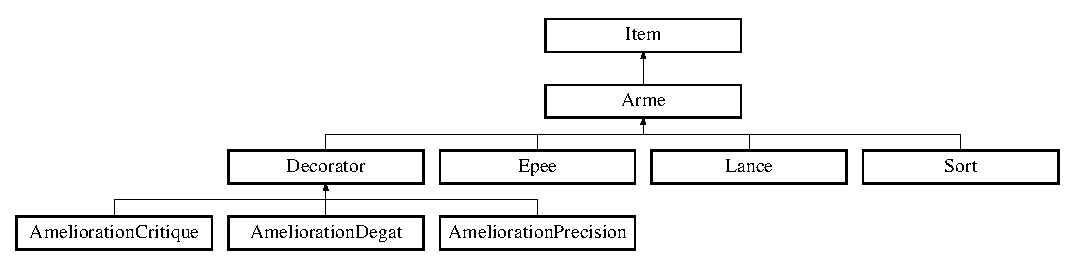
\includegraphics[height=3.132867cm]{classItem}
\end{center}
\end{figure}
\subsection*{Fonctions membres publiques}
\begin{DoxyCompactItemize}
\item 
\hyperlink{classItem_a9b72af940c9e375038de5ea420f471f0}{Item} (std\-::string nom\-Item)
\begin{DoxyCompactList}\small\item\em Constructeur d'item (\hyperlink{classClasse}{Classe} abstraite) \end{DoxyCompactList}\item 
\hypertarget{classItem_a11663c84075b78c3ae5e30fdfcd7c458}{virtual \hyperlink{classItem_a11663c84075b78c3ae5e30fdfcd7c458}{$\sim$\-Item} ()}\label{classItem_a11663c84075b78c3ae5e30fdfcd7c458}

\begin{DoxyCompactList}\small\item\em Le destructeur de l'item. \end{DoxyCompactList}\item 
std\-::string \hyperlink{classItem_abd58e71362b471f03b4d520c10c1545d}{get\-Nom\-Item} ()
\begin{DoxyCompactList}\small\item\em getter de nom\-Item \end{DoxyCompactList}\end{DoxyCompactItemize}
\subsection*{Attributs protégés}
\begin{DoxyCompactItemize}
\item 
\hypertarget{classItem_a068ef6dbb8cea714174d6956e89b1042}{std\-::string {\bfseries nom\-Item}}\label{classItem_a068ef6dbb8cea714174d6956e89b1042}

\end{DoxyCompactItemize}


\subsection{Documentation des constructeurs et destructeur}
\hypertarget{classItem_a9b72af940c9e375038de5ea420f471f0}{\index{Item@{Item}!Item@{Item}}
\index{Item@{Item}!Item@{Item}}
\subsubsection[{Item}]{\setlength{\rightskip}{0pt plus 5cm}Item\-::\-Item (
\begin{DoxyParamCaption}
\item[{std\-::string}]{nom\-Item}
\end{DoxyParamCaption}
)}}\label{classItem_a9b72af940c9e375038de5ea420f471f0}


Constructeur d'item (\hyperlink{classClasse}{Classe} abstraite) 


\begin{DoxyParams}{Paramètres}
{\em nom\-Arme} & Le nom de l'item. \\
\hline
\end{DoxyParams}


\subsection{Documentation des fonctions membres}
\hypertarget{classItem_abd58e71362b471f03b4d520c10c1545d}{\index{Item@{Item}!get\-Nom\-Item@{get\-Nom\-Item}}
\index{get\-Nom\-Item@{get\-Nom\-Item}!Item@{Item}}
\subsubsection[{get\-Nom\-Item}]{\setlength{\rightskip}{0pt plus 5cm}std\-::string Item\-::get\-Nom\-Item (
\begin{DoxyParamCaption}
{}
\end{DoxyParamCaption}
)}}\label{classItem_abd58e71362b471f03b4d520c10c1545d}


getter de nom\-Item 

\begin{DoxyReturn}{Renvoie}
std\-::string nom de l'item 
\end{DoxyReturn}


La documentation de cette classe a été générée à partir des fichiers suivants \-:\begin{DoxyCompactItemize}
\item 
Item.\-hpp\item 
Item.\-cpp\end{DoxyCompactItemize}

\hypertarget{classLance}{\section{Référence de la classe Lance}
\label{classLance}\index{Lance@{Lance}}
}
Graphe d'héritage de Lance\-:\begin{figure}[H]
\begin{center}
\leavevmode
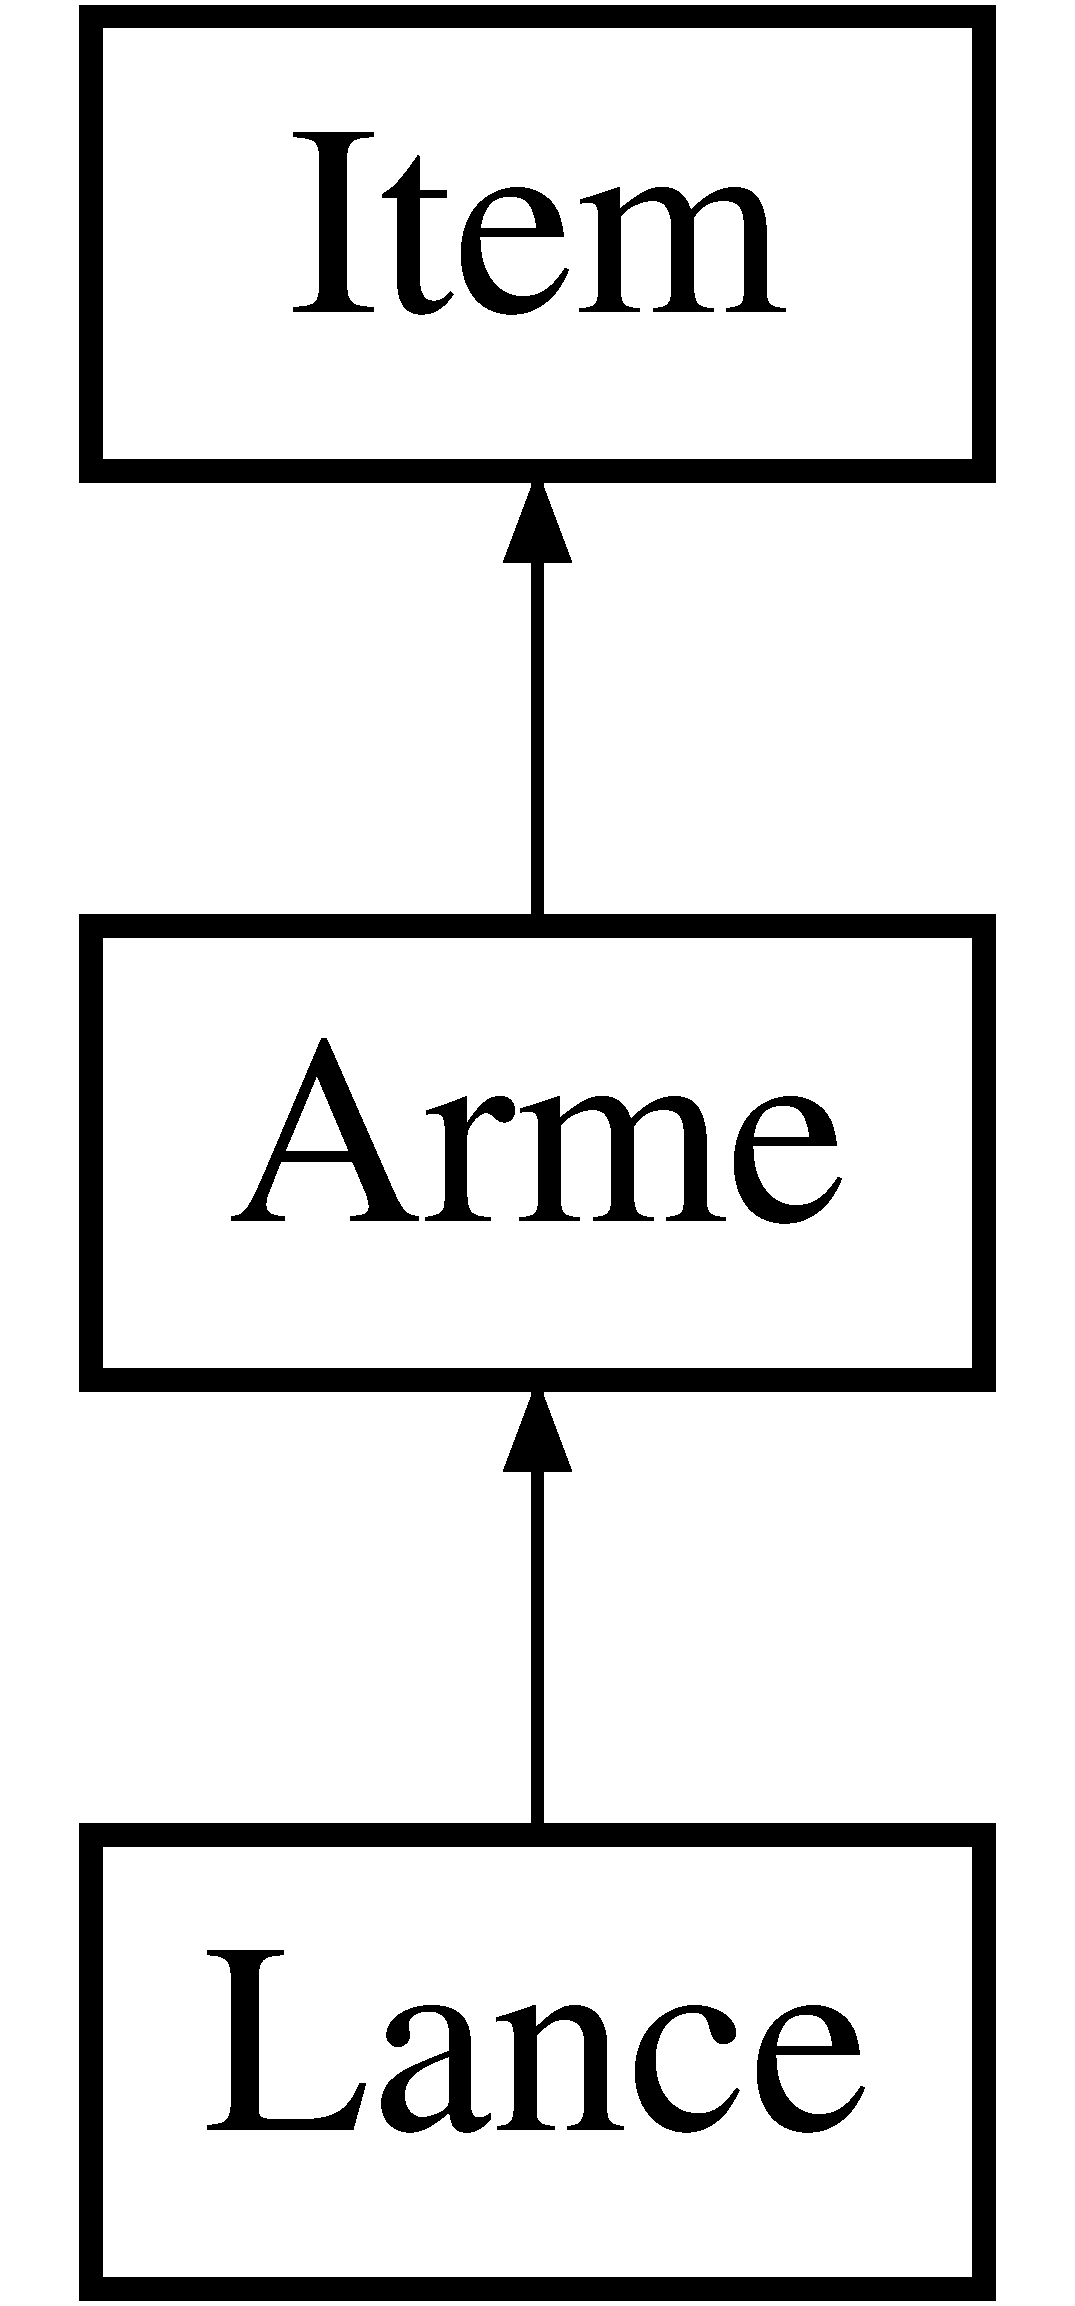
\includegraphics[height=3.000000cm]{classLance}
\end{center}
\end{figure}
\subsection*{Fonctions membres publiques}
\begin{DoxyCompactItemize}
\item 
\hypertarget{classLance_aafa988062f9318f245741be0b5307fe5}{\hyperlink{classLance_aafa988062f9318f245741be0b5307fe5}{Lance} (std\-::string nom\-Arme, int puissance, int precision, int critique, bool est\-Magique, int prix)}\label{classLance_aafa988062f9318f245741be0b5307fe5}

\begin{DoxyCompactList}\small\item\em Construit une arme de type 1. \end{DoxyCompactList}\end{DoxyCompactItemize}
\subsection*{Membres hérités additionnels}


La documentation de cette classe a été générée à partir des fichiers suivants \-:\begin{DoxyCompactItemize}
\item 
Armes.\-hpp\item 
Armes.\-cpp\end{DoxyCompactItemize}

\hypertarget{classMarchand}{\section{Référence de la classe Marchand}
\label{classMarchand}\index{Marchand@{Marchand}}
}
\subsection*{Fonctions membres publiques}
\begin{DoxyCompactItemize}
\item 
\hyperlink{classMarchand_ad4ab208a21ab8adeb741f3f4d1bf3c5c}{Marchand} (std\-::vector$<$ \hyperlink{classArme}{Arme} $\ast$ $>$ vec\-Insatancieur)
\begin{DoxyCompactList}\small\item\em Le constructeur du marchand. \end{DoxyCompactList}\item 
\hypertarget{classMarchand_ab5294b5de6ce2bfff99f2b29d9a2f4ba}{\hyperlink{classMarchand_ab5294b5de6ce2bfff99f2b29d9a2f4ba}{$\sim$\-Marchand} ()}\label{classMarchand_ab5294b5de6ce2bfff99f2b29d9a2f4ba}

\begin{DoxyCompactList}\small\item\em Le destructeur du marchand. \end{DoxyCompactList}\item 
void \hyperlink{classMarchand_a6e8fbc688e23a97d761359cb36801564}{marcher} (\hyperlink{classPersonnage}{Personnage} $\ast$perso)
\begin{DoxyCompactList}\small\item\em fait le commerce avec le marchand. \end{DoxyCompactList}\item 
void \hyperlink{classMarchand_afec086e17a2df2c16f730a7b22c04fd9}{afficher\-Menu} (\hyperlink{classPersonnage}{Personnage} $\ast$perso)
\begin{DoxyCompactList}\small\item\em afficher le menu et appelle les methodes d'achat ou de upgrade d'arme \end{DoxyCompactList}\item 
void \hyperlink{classMarchand_afa159699ab3a8f374f67775f3f0f2d56}{achat} (\hyperlink{classPersonnage}{Personnage} $\ast$perso)
\begin{DoxyCompactList}\small\item\em affiche l'inventaire du marchand et determine si le joueur peut acheter. \end{DoxyCompactList}\item 
void \hyperlink{classMarchand_a0346e8673ad63cc9ff3d49e805c25645}{ameliorer} (\hyperlink{classPersonnage}{Personnage} $\ast$perso)
\begin{DoxyCompactList}\small\item\em Afficher le menu d'amelioration et effectuer les ameliorations. \end{DoxyCompactList}\item 
\hyperlink{classArme}{Arme} $\ast$ \hyperlink{classMarchand_ab91a5c2933a62a05d2c0a4926fcaadd0}{get\-Arme} (std\-::string nom\-Arme)
\begin{DoxyCompactList}\small\item\em retour une arme si elle est presente dans l'inventaire du marchand. \end{DoxyCompactList}\item 
int \hyperlink{classMarchand_aa3167b6744857b841091896e8e791383}{min} (int a, int b)
\begin{DoxyCompactList}\small\item\em Revoi la plus petite des deux valeures. \end{DoxyCompactList}\item 
bool \hyperlink{classMarchand_a939b005d84cce6fd81adaa037025eb51}{contains} (std\-::vector$<$ \hyperlink{classArme}{Arme} $\ast$ $>$ vec, \hyperlink{classArme}{Arme} $\ast$arme)
\begin{DoxyCompactList}\small\item\em Test si l'arme est poséder par le marchand. \end{DoxyCompactList}\end{DoxyCompactItemize}


\subsection{Documentation des constructeurs et destructeur}
\hypertarget{classMarchand_ad4ab208a21ab8adeb741f3f4d1bf3c5c}{\index{Marchand@{Marchand}!Marchand@{Marchand}}
\index{Marchand@{Marchand}!Marchand@{Marchand}}
\subsubsection[{Marchand}]{\setlength{\rightskip}{0pt plus 5cm}Marchand\-::\-Marchand (
\begin{DoxyParamCaption}
\item[{std\-::vector$<$ {\bf Arme} $\ast$ $>$}]{vec\-Insatancieur}
\end{DoxyParamCaption}
)}}\label{classMarchand_ad4ab208a21ab8adeb741f3f4d1bf3c5c}


Le constructeur du marchand. 

fait de l'aleatoire pour l'ajout des armes pour varier son inventaire 
\begin{DoxyParams}{Paramètres}
{\em vec\-Insatancieur} & les armes du machand. \\
\hline
\end{DoxyParams}


\subsection{Documentation des fonctions membres}
\hypertarget{classMarchand_afa159699ab3a8f374f67775f3f0f2d56}{\index{Marchand@{Marchand}!achat@{achat}}
\index{achat@{achat}!Marchand@{Marchand}}
\subsubsection[{achat}]{\setlength{\rightskip}{0pt plus 5cm}void Marchand\-::achat (
\begin{DoxyParamCaption}
\item[{{\bf Personnage} $\ast$}]{perso}
\end{DoxyParamCaption}
)}}\label{classMarchand_afa159699ab3a8f374f67775f3f0f2d56}


affiche l'inventaire du marchand et determine si le joueur peut acheter. 


\begin{DoxyParams}{Paramètres}
{\em perso} & Personnage$\ast$ le pigeon qui achete. \\
\hline
\end{DoxyParams}
\hypertarget{classMarchand_afec086e17a2df2c16f730a7b22c04fd9}{\index{Marchand@{Marchand}!afficher\-Menu@{afficher\-Menu}}
\index{afficher\-Menu@{afficher\-Menu}!Marchand@{Marchand}}
\subsubsection[{afficher\-Menu}]{\setlength{\rightskip}{0pt plus 5cm}void Marchand\-::afficher\-Menu (
\begin{DoxyParamCaption}
\item[{{\bf Personnage} $\ast$}]{perso}
\end{DoxyParamCaption}
)}}\label{classMarchand_afec086e17a2df2c16f730a7b22c04fd9}


afficher le menu et appelle les methodes d'achat ou de upgrade d'arme 


\begin{DoxyParams}{Paramètres}
{\em perso} & Personnage$\ast$ le pigeon qui achete. \\
\hline
\end{DoxyParams}
\hypertarget{classMarchand_a0346e8673ad63cc9ff3d49e805c25645}{\index{Marchand@{Marchand}!ameliorer@{ameliorer}}
\index{ameliorer@{ameliorer}!Marchand@{Marchand}}
\subsubsection[{ameliorer}]{\setlength{\rightskip}{0pt plus 5cm}void Marchand\-::ameliorer (
\begin{DoxyParamCaption}
\item[{{\bf Personnage} $\ast$}]{perso}
\end{DoxyParamCaption}
)}}\label{classMarchand_a0346e8673ad63cc9ff3d49e805c25645}


Afficher le menu d'amelioration et effectuer les ameliorations. 


\begin{DoxyParams}{Paramètres}
{\em perso} & Personnage$\ast$ le perso qui va avoir une arme ameliorer \\
\hline
\end{DoxyParams}
\hypertarget{classMarchand_a939b005d84cce6fd81adaa037025eb51}{\index{Marchand@{Marchand}!contains@{contains}}
\index{contains@{contains}!Marchand@{Marchand}}
\subsubsection[{contains}]{\setlength{\rightskip}{0pt plus 5cm}bool Marchand\-::contains (
\begin{DoxyParamCaption}
\item[{std\-::vector$<$ {\bf Arme} $\ast$ $>$}]{vec, }
\item[{{\bf Arme} $\ast$}]{arme}
\end{DoxyParamCaption}
)}}\label{classMarchand_a939b005d84cce6fd81adaa037025eb51}


Test si l'arme est poséder par le marchand. 


\begin{DoxyParams}{Paramètres}
{\em vec} & le vecteur d'arme du amrchand. \\
\hline
{\em l'arme} & à tester. \\
\hline
\end{DoxyParams}
\begin{DoxyReturn}{Renvoie}
vrais si le marchad possède l'arme. 
\end{DoxyReturn}
\hypertarget{classMarchand_ab91a5c2933a62a05d2c0a4926fcaadd0}{\index{Marchand@{Marchand}!get\-Arme@{get\-Arme}}
\index{get\-Arme@{get\-Arme}!Marchand@{Marchand}}
\subsubsection[{get\-Arme}]{\setlength{\rightskip}{0pt plus 5cm}{\bf Arme} $\ast$ Marchand\-::get\-Arme (
\begin{DoxyParamCaption}
\item[{std\-::string}]{nom\-Arme}
\end{DoxyParamCaption}
)}}\label{classMarchand_ab91a5c2933a62a05d2c0a4926fcaadd0}


retour une arme si elle est presente dans l'inventaire du marchand. 


\begin{DoxyParams}{Paramètres}
{\em nom\-Arme} & std\-::string le nom de l'arme que l'on recherche \\
\hline
\end{DoxyParams}
\begin{DoxyReturn}{Renvoie}
Arme$\ast$ l'arme ou un nullptr 
\end{DoxyReturn}
\hypertarget{classMarchand_a6e8fbc688e23a97d761359cb36801564}{\index{Marchand@{Marchand}!marcher@{marcher}}
\index{marcher@{marcher}!Marchand@{Marchand}}
\subsubsection[{marcher}]{\setlength{\rightskip}{0pt plus 5cm}void Marchand\-::marcher (
\begin{DoxyParamCaption}
\item[{{\bf Personnage} $\ast$}]{perso}
\end{DoxyParamCaption}
)}}\label{classMarchand_a6e8fbc688e23a97d761359cb36801564}


fait le commerce avec le marchand. 

appelle la methode affichermenu 
\begin{DoxyParams}{Paramètres}
{\em perso} & Personnage$\ast$ le pigeon qui achete. \\
\hline
\end{DoxyParams}
\hypertarget{classMarchand_aa3167b6744857b841091896e8e791383}{\index{Marchand@{Marchand}!min@{min}}
\index{min@{min}!Marchand@{Marchand}}
\subsubsection[{min}]{\setlength{\rightskip}{0pt plus 5cm}int Marchand\-::min (
\begin{DoxyParamCaption}
\item[{int}]{a, }
\item[{int}]{b}
\end{DoxyParamCaption}
)}}\label{classMarchand_aa3167b6744857b841091896e8e791383}


Revoi la plus petite des deux valeures. 


\begin{DoxyParams}{Paramètres}
{\em a} & le premier entier. \\
\hline
{\em b} & le second argument. \\
\hline
\end{DoxyParams}
\begin{DoxyReturn}{Renvoie}
a ou b. 
\end{DoxyReturn}


La documentation de cette classe a été générée à partir des fichiers suivants \-:\begin{DoxyCompactItemize}
\item 
Marchand.\-hpp\item 
Marchand.\-cpp\end{DoxyCompactItemize}

\hypertarget{classPersonnage}{\section{Référence de la classe Personnage}
\label{classPersonnage}\index{Personnage@{Personnage}}
}
\subsection*{Fonctions membres publiques}
\begin{DoxyCompactItemize}
\item 
\hyperlink{classPersonnage_af67a53c849a176a4dd642bb6b634833e}{Personnage} (std\-::vector$<$ int $>$ s, std\-::string n, \hyperlink{classClasseHeroique}{Classe\-Heroique} $\ast$c, \hyperlink{classRace}{Race} $\ast$r, bool est\-Femme, int niveau)
\begin{DoxyCompactList}\small\item\em Constructeur de \hyperlink{classPersonnage}{Personnage}. \end{DoxyCompactList}\item 
\hyperlink{classPersonnage_a05bdf2a469885bb1fbb6c2e8f98972ab}{$\sim$\-Personnage} ()
\begin{DoxyCompactList}\small\item\em Destructeur de personnage. \end{DoxyCompactList}\item 
void \hyperlink{classPersonnage_ac1a65837596032eba2af5a4b9309b114}{action\-Combat} (\hyperlink{classPersonnage}{Personnage} $\ast$cible)
\begin{DoxyCompactList}\small\item\em Menu d'action du joueur. \end{DoxyCompactList}\item 
void \hyperlink{classPersonnage_a56baf3c31093afa4f232c6ca0d434d6c}{combat\-Automatique} (\hyperlink{classPersonnage}{Personnage} $\ast$cible)
\begin{DoxyCompactList}\small\item\em la methode de gestion prise de decision pour l'I\-A \end{DoxyCompactList}\item 
void \hyperlink{classPersonnage_ae9f35f04c2e15c98d97db9675d531d46}{change\-Posture} ()
\begin{DoxyCompactList}\small\item\em Menu de changement de posture. \end{DoxyCompactList}\item 
bool \hyperlink{classPersonnage_a2c731ad41a9d720df7d818a6705a3f3c}{se\-Soigner} ()
\begin{DoxyCompactList}\small\item\em permet de se soigner \end{DoxyCompactList}\item 
void \hyperlink{classPersonnage_a524d0e177e9dfd472189ef60bb9f7828}{set\-Arme\-Equiper} (\hyperlink{classArme}{Arme} $\ast$a)
\begin{DoxyCompactList}\small\item\em Change l'arme du personnage. \end{DoxyCompactList}\item 
void \hyperlink{classPersonnage_a356317bcbf60de8f579a7816d3112f19}{set\-Classe\-Actuelle} (\hyperlink{classClasse}{Classe} $\ast$classe)
\begin{DoxyCompactList}\small\item\em setter de classe\-Actuelle \end{DoxyCompactList}\item 
void \hyperlink{classPersonnage_a77a2868f0ebe1747adb0395ad8c49d4e}{set\-Classe\-Parangon} (\hyperlink{classClasse}{Classe} $\ast$classe)
\begin{DoxyCompactList}\small\item\em setter de classe\-Parangon \end{DoxyCompactList}\item 
void \hyperlink{classPersonnage_a2c9b4bdc2a17ee4b53ba1df442948adb}{set\-Classe\-Divine} (\hyperlink{classClasse}{Classe} $\ast$classe)
\begin{DoxyCompactList}\small\item\em setter de classe\-Divine \end{DoxyCompactList}\item 
void \hyperlink{classPersonnage_a89bee8eb8c2c0e6b7b47f78a93c6d96a}{monter\-Niveau} ()
\begin{DoxyCompactList}\small\item\em S000000000\-N !!! \end{DoxyCompactList}\item 
int \hyperlink{classPersonnage_a2724dcc386b3858caec89c0a76977d11}{update\-Degat} ()
\begin{DoxyCompactList}\small\item\em calcul les degats \end{DoxyCompactList}\item 
int \hyperlink{classPersonnage_abfe657430f5cf3c4d88e66fba39f574b}{update\-Precision} ()
\begin{DoxyCompactList}\small\item\em calcul la precision \end{DoxyCompactList}\item 
int \hyperlink{classPersonnage_ab96e4988ee1e14a3e5e728305142b087}{update\-Critique} ()
\begin{DoxyCompactList}\small\item\em calcul la valeur de critique \end{DoxyCompactList}\item 
int \hyperlink{classPersonnage_a07c30a08ae68fd69e19bb536853d9fd5}{update\-Esquive} ()
\begin{DoxyCompactList}\small\item\em calcul l'esquive \end{DoxyCompactList}\item 
void \hyperlink{classPersonnage_af735b2cf101b1cabbbd14cc24b6a935d}{update\-Niveau} ()
\begin{DoxyCompactList}\small\item\em calcul l'experience et appelle la methode de monter de niveau \end{DoxyCompactList}\item 
\hypertarget{classPersonnage_a1498effa56d179e4f98b2715201f6260}{void \hyperlink{classPersonnage_a1498effa56d179e4f98b2715201f6260}{update\-P\-V} ()}\label{classPersonnage_a1498effa56d179e4f98b2715201f6260}

\begin{DoxyCompactList}\small\item\em verifie que les pv sont inferieurs au pv\-Max \end{DoxyCompactList}\item 
void \hyperlink{classPersonnage_ac0c4df6c3f5858a254ffe2687447e9da}{prendre\-Degat} (int degat)
\begin{DoxyCompactList}\small\item\em Affiche et retire les pv perdut après mis a jour via la posture. \end{DoxyCompactList}\item 
void \hyperlink{classPersonnage_a1d43355b9b9aade85f3bb5ffec06b840}{attaquer} (\hyperlink{classPersonnage}{Personnage} $\ast$cible)
\begin{DoxyCompactList}\small\item\em determine si le personnage touche puis calcule les degats \end{DoxyCompactList}\item 
void \hyperlink{classPersonnage_a37a51c8be3bd343234f4ef009239f8ee}{mourant} ()
\begin{DoxyCompactList}\small\item\em determine la mort du perso en fonction de sa classe \end{DoxyCompactList}\item 
void \hyperlink{classPersonnage_a8944e1085ad9872619b66d484dd1b1f9}{mod\-Stat} (int stat, int modificateur)
\begin{DoxyCompactList}\small\item\em modifie une stat a une position donner d'une valeur donner puis met a jour les statistique deriver \end{DoxyCompactList}\item 
\hyperlink{classRace}{Race} $\ast$ \hyperlink{classPersonnage_afbe2ae0138f81a92e24db419bcbea9d5}{get\-Race} ()
\begin{DoxyCompactList}\small\item\em getter de Race$\ast$ \end{DoxyCompactList}\item 
std\-::string \hyperlink{classPersonnage_ac0fbc92a7e930ae26148e5e5247e1494}{get\-Nom} ()
\begin{DoxyCompactList}\small\item\em getter de Nom \end{DoxyCompactList}\item 
\hyperlink{classClasse}{Classe} $\ast$ \hyperlink{classPersonnage_aa306767186f6003aadf90a6e213334e7}{get\-Classe\-Actuelle} ()
\begin{DoxyCompactList}\small\item\em getter de Classe\-Actuelle$\ast$ \end{DoxyCompactList}\item 
bool \hyperlink{classPersonnage_abb94f081188ed8db8a359c71cb1fad15}{get\-Est\-Femme} ()
\begin{DoxyCompactList}\small\item\em getter de est\-Femme \end{DoxyCompactList}\item 
\hypertarget{classPersonnage_a7bddda23478b2aa48404790dde0aeefb}{void \hyperlink{classPersonnage_a7bddda23478b2aa48404790dde0aeefb}{update\-Statistique} ()}\label{classPersonnage_a7bddda23478b2aa48404790dde0aeefb}

\begin{DoxyCompactList}\small\item\em appelle les autres methodes d'update \end{DoxyCompactList}\item 
std\-::vector$<$ int $>$ \hyperlink{classPersonnage_aa3e7743cb3b74039adcdea14f44c6352}{get\-Statistique} ()
\begin{DoxyCompactList}\small\item\em getter de statistique \end{DoxyCompactList}\item 
std\-::vector$<$ int $>$ \hyperlink{classPersonnage_a5bf62bc5df34f14f3c0c9717b61498d5}{get\-Statistique\-Derive} ()
\begin{DoxyCompactList}\small\item\em getter de statistique\-Derive retour les statistique\-Derive Après avoir fait une mise a jour \end{DoxyCompactList}\item 
\hyperlink{classClasse}{Classe} $\ast$ \hyperlink{classPersonnage_ae9d4cf3dc0c47e5652df837c7839efd8}{get\-Classe\-Heroique} ()
\begin{DoxyCompactList}\small\item\em getter de classe\-Heroique$\ast$ \end{DoxyCompactList}\item 
\hyperlink{classClasse}{Classe} $\ast$ \hyperlink{classPersonnage_ad63aa2e6903143a494c72298c90eb7ba}{get\-Classe\-Parangon} ()
\begin{DoxyCompactList}\small\item\em getter de classe\-Parangon$\ast$ \end{DoxyCompactList}\item 
\hyperlink{classClasse}{Classe} $\ast$ \hyperlink{classPersonnage_af072c7506dc955ba44abbacf29c7a4bf}{get\-Classe\-Divine} ()
\begin{DoxyCompactList}\small\item\em getter de classe\-Divine$\ast$ \end{DoxyCompactList}\item 
\hypertarget{classPersonnage_ab3747da2ed7044c6bd2b62fd439d6ad0}{void \hyperlink{classPersonnage_ab3747da2ed7044c6bd2b62fd439d6ad0}{afficher\-Stat} ()}\label{classPersonnage_ab3747da2ed7044c6bd2b62fd439d6ad0}

\begin{DoxyCompactList}\small\item\em afficher les statistiques puis les statistiques derivées du perso \end{DoxyCompactList}\item 
void \hyperlink{classPersonnage_abc49c5153087cee2e1302e73fb198272}{promotion} (\hyperlink{classClasse}{Classe} $\ast$classe)
\begin{DoxyCompactList}\small\item\em effectue un changement d'etat \char`\"{}vers le haut\char`\"{} si les conditions sont valide \end{DoxyCompactList}\item 
\hypertarget{classPersonnage_abcf2887d6670a7d0486bf08eb0b32304}{void \hyperlink{classPersonnage_abcf2887d6670a7d0486bf08eb0b32304}{decheance} ()}\label{classPersonnage_abcf2887d6670a7d0486bf08eb0b32304}

\begin{DoxyCompactList}\small\item\em effectue un changement d'etat \char`\"{}vers le bas\char`\"{} si on est pas en Heroique \end{DoxyCompactList}\item 
int \hyperlink{classPersonnage_a0024a1f71a6f0c252be639463ac39c7c}{critique} (int degat, \hyperlink{classPersonnage}{Personnage} $\ast$cible)
\begin{DoxyCompactList}\small\item\em Determine si le coups est un coups critique. \end{DoxyCompactList}\item 
bool \hyperlink{classPersonnage_ad44fed592109b5804b1246f3d6a186f3}{est\-Mort} ()
\begin{DoxyCompactList}\small\item\em indique si le perso est mort ie pv negatif ou nul \end{DoxyCompactList}\item 
void \hyperlink{classPersonnage_a25b1a649e9322aac97ec55630959c8cc}{mod\-Argent} (int argent)
\begin{DoxyCompactList}\small\item\em modifie l'argent selon un entier donner en param \end{DoxyCompactList}\item 
bool \hyperlink{classPersonnage_a9cfba1f94fc07bc9f42fc50901e143f9}{possede\-Assez\-Argent} (int argent)
\begin{DoxyCompactList}\small\item\em indique si le perso a assez d'argent \end{DoxyCompactList}\item 
int \hyperlink{classPersonnage_ab2396463311e9585a42f050273df7751}{get\-Argent} ()
\begin{DoxyCompactList}\small\item\em getter d'argent \end{DoxyCompactList}\item 
\hyperlink{classArme}{Arme} $\ast$ \hyperlink{classPersonnage_ae6268f94bc88685bfab88f15ba3ec9f1}{get\-Arme\-Actuelle} ()
\begin{DoxyCompactList}\small\item\em getter de l'arme actuelle du perso \end{DoxyCompactList}\end{DoxyCompactItemize}


\subsection{Documentation des constructeurs et destructeur}
\hypertarget{classPersonnage_af67a53c849a176a4dd642bb6b634833e}{\index{Personnage@{Personnage}!Personnage@{Personnage}}
\index{Personnage@{Personnage}!Personnage@{Personnage}}
\subsubsection[{Personnage}]{\setlength{\rightskip}{0pt plus 5cm}Personnage\-::\-Personnage (
\begin{DoxyParamCaption}
\item[{std\-::vector$<$ int $>$}]{s, }
\item[{std\-::string}]{n, }
\item[{{\bf Classe\-Heroique} $\ast$}]{c, }
\item[{{\bf Race} $\ast$}]{r, }
\item[{bool}]{est\-Femme, }
\item[{int}]{niveau}
\end{DoxyParamCaption}
)}}\label{classPersonnage_af67a53c849a176a4dd642bb6b634833e}


Constructeur de \hyperlink{classPersonnage}{Personnage}. 

Sers a crée un personnage via les paramètres decrit ci desous, à initialiser ses statistiques ainsi que sa classe\-Actuelle et initialiser sa posture a \hyperlink{classDefenseur}{Defenseur} 
\begin{DoxyParams}{Paramètres}
{\em s} & vector$<$int$>$ Le vector de stat de base du perso \\
\hline
{\em n} & string Le nom du personnage \\
\hline
{\em c} & Classe\-Heroique$\ast$ Le pointeur vers la classe heroique(ne peut pas être modifier) \\
\hline
{\em r} & Race$\ast$ La pointeur vers la race du personnage \\
\hline
{\em est\-Femme} & bool vrai si le personnage est une femme \\
\hline
{\em niveau} & int indique le niveau du personnage(normale 1 au debut) \\
\hline
\end{DoxyParams}
\hypertarget{classPersonnage_a05bdf2a469885bb1fbb6c2e8f98972ab}{\index{Personnage@{Personnage}!$\sim$\-Personnage@{$\sim$\-Personnage}}
\index{$\sim$\-Personnage@{$\sim$\-Personnage}!Personnage@{Personnage}}
\subsubsection[{$\sim$\-Personnage}]{\setlength{\rightskip}{0pt plus 5cm}Personnage\-::$\sim$\-Personnage (
\begin{DoxyParamCaption}
{}
\end{DoxyParamCaption}
)}}\label{classPersonnage_a05bdf2a469885bb1fbb6c2e8f98972ab}


Destructeur de personnage. 

remet tout les pointeurs a nullptr car les objets doivent être detruit dans l'instancieur 

\subsection{Documentation des fonctions membres}
\hypertarget{classPersonnage_ac1a65837596032eba2af5a4b9309b114}{\index{Personnage@{Personnage}!action\-Combat@{action\-Combat}}
\index{action\-Combat@{action\-Combat}!Personnage@{Personnage}}
\subsubsection[{action\-Combat}]{\setlength{\rightskip}{0pt plus 5cm}void Personnage\-::action\-Combat (
\begin{DoxyParamCaption}
\item[{{\bf Personnage} $\ast$}]{cible}
\end{DoxyParamCaption}
)}}\label{classPersonnage_ac1a65837596032eba2af5a4b9309b114}


Menu d'action du joueur. 

affiche le menu et en fonction d'une entré clavier appelle une methode specifique 1 pour attaquer, 2 pour se soigner, 3 pour changer de posture 
\begin{DoxyParams}{Paramètres}
{\em cible} & Personnage$\ast$ notre ennemie actuelle \\
\hline
\end{DoxyParams}
\hypertarget{classPersonnage_a1d43355b9b9aade85f3bb5ffec06b840}{\index{Personnage@{Personnage}!attaquer@{attaquer}}
\index{attaquer@{attaquer}!Personnage@{Personnage}}
\subsubsection[{attaquer}]{\setlength{\rightskip}{0pt plus 5cm}void Personnage\-::attaquer (
\begin{DoxyParamCaption}
\item[{{\bf Personnage} $\ast$}]{cible}
\end{DoxyParamCaption}
)}}\label{classPersonnage_a1d43355b9b9aade85f3bb5ffec06b840}


determine si le personnage touche puis calcule les degats 

les calculs se fait viens du rng 
\begin{DoxyParams}{Paramètres}
{\em cible} & Personnage$\ast$ l'ennemie actuelle \\
\hline
\end{DoxyParams}
\hypertarget{classPersonnage_ae9f35f04c2e15c98d97db9675d531d46}{\index{Personnage@{Personnage}!change\-Posture@{change\-Posture}}
\index{change\-Posture@{change\-Posture}!Personnage@{Personnage}}
\subsubsection[{change\-Posture}]{\setlength{\rightskip}{0pt plus 5cm}void Personnage\-::change\-Posture (
\begin{DoxyParamCaption}
{}
\end{DoxyParamCaption}
)}}\label{classPersonnage_ae9f35f04c2e15c98d97db9675d531d46}


Menu de changement de posture. 

affiche le menu et en fonction d'une entré clavier crée une nouvelle posture \begin{DoxyRefDesc}{Bogue}
\item[\hyperlink{bug__bug000002}{Bogue}]need un delete de la posture ? \end{DoxyRefDesc}
\hypertarget{classPersonnage_a56baf3c31093afa4f232c6ca0d434d6c}{\index{Personnage@{Personnage}!combat\-Automatique@{combat\-Automatique}}
\index{combat\-Automatique@{combat\-Automatique}!Personnage@{Personnage}}
\subsubsection[{combat\-Automatique}]{\setlength{\rightskip}{0pt plus 5cm}void Personnage\-::combat\-Automatique (
\begin{DoxyParamCaption}
\item[{{\bf Personnage} $\ast$}]{cible}
\end{DoxyParamCaption}
)}}\label{classPersonnage_a56baf3c31093afa4f232c6ca0d434d6c}


la methode de gestion prise de decision pour l'I\-A 


\begin{DoxyParams}{Paramètres}
{\em cible} & Personnage$\ast$ l'ennemie actuelle de l'I\-A (à l'heure actuelle le joueur) \\
\hline
\end{DoxyParams}
\hypertarget{classPersonnage_a0024a1f71a6f0c252be639463ac39c7c}{\index{Personnage@{Personnage}!critique@{critique}}
\index{critique@{critique}!Personnage@{Personnage}}
\subsubsection[{critique}]{\setlength{\rightskip}{0pt plus 5cm}int Personnage\-::critique (
\begin{DoxyParamCaption}
\item[{int}]{degat, }
\item[{{\bf Personnage} $\ast$}]{cible}
\end{DoxyParamCaption}
)}}\label{classPersonnage_a0024a1f71a6f0c252be639463ac39c7c}


Determine si le coups est un coups critique. 


\begin{DoxyParams}{Paramètres}
{\em degat} & int les degat avant le calcule du critique \\
\hline
{\em cible} & Personnage$\ast$ notre cible actuelle \\
\hline
\end{DoxyParams}
\hypertarget{classPersonnage_ad44fed592109b5804b1246f3d6a186f3}{\index{Personnage@{Personnage}!est\-Mort@{est\-Mort}}
\index{est\-Mort@{est\-Mort}!Personnage@{Personnage}}
\subsubsection[{est\-Mort}]{\setlength{\rightskip}{0pt plus 5cm}bool Personnage\-::est\-Mort (
\begin{DoxyParamCaption}
{}
\end{DoxyParamCaption}
)}}\label{classPersonnage_ad44fed592109b5804b1246f3d6a186f3}


indique si le perso est mort ie pv negatif ou nul 

\begin{DoxyReturn}{Renvoie}
vrai si les pv sont negatif ou nul 
\end{DoxyReturn}
\hypertarget{classPersonnage_ab2396463311e9585a42f050273df7751}{\index{Personnage@{Personnage}!get\-Argent@{get\-Argent}}
\index{get\-Argent@{get\-Argent}!Personnage@{Personnage}}
\subsubsection[{get\-Argent}]{\setlength{\rightskip}{0pt plus 5cm}int Personnage\-::get\-Argent (
\begin{DoxyParamCaption}
{}
\end{DoxyParamCaption}
)}}\label{classPersonnage_ab2396463311e9585a42f050273df7751}


getter d'argent 

\begin{DoxyReturn}{Renvoie}
argent int l'argent du perso 
\end{DoxyReturn}
\hypertarget{classPersonnage_ae6268f94bc88685bfab88f15ba3ec9f1}{\index{Personnage@{Personnage}!get\-Arme\-Actuelle@{get\-Arme\-Actuelle}}
\index{get\-Arme\-Actuelle@{get\-Arme\-Actuelle}!Personnage@{Personnage}}
\subsubsection[{get\-Arme\-Actuelle}]{\setlength{\rightskip}{0pt plus 5cm}{\bf Arme} $\ast$ Personnage\-::get\-Arme\-Actuelle (
\begin{DoxyParamCaption}
{}
\end{DoxyParamCaption}
)}}\label{classPersonnage_ae6268f94bc88685bfab88f15ba3ec9f1}


getter de l'arme actuelle du perso 

\begin{DoxyReturn}{Renvoie}
arme\-Equiper Arme$\ast$ 
\end{DoxyReturn}
\hypertarget{classPersonnage_aa306767186f6003aadf90a6e213334e7}{\index{Personnage@{Personnage}!get\-Classe\-Actuelle@{get\-Classe\-Actuelle}}
\index{get\-Classe\-Actuelle@{get\-Classe\-Actuelle}!Personnage@{Personnage}}
\subsubsection[{get\-Classe\-Actuelle}]{\setlength{\rightskip}{0pt plus 5cm}{\bf Classe} $\ast$ Personnage\-::get\-Classe\-Actuelle (
\begin{DoxyParamCaption}
{}
\end{DoxyParamCaption}
)}}\label{classPersonnage_aa306767186f6003aadf90a6e213334e7}


getter de Classe\-Actuelle$\ast$ 

\begin{DoxyReturn}{Renvoie}
Classe\-Actuelle$\ast$ le pointeur de classe actuelle du perso 
\end{DoxyReturn}
\hypertarget{classPersonnage_af072c7506dc955ba44abbacf29c7a4bf}{\index{Personnage@{Personnage}!get\-Classe\-Divine@{get\-Classe\-Divine}}
\index{get\-Classe\-Divine@{get\-Classe\-Divine}!Personnage@{Personnage}}
\subsubsection[{get\-Classe\-Divine}]{\setlength{\rightskip}{0pt plus 5cm}{\bf Classe} $\ast$ Personnage\-::get\-Classe\-Divine (
\begin{DoxyParamCaption}
{}
\end{DoxyParamCaption}
)}}\label{classPersonnage_af072c7506dc955ba44abbacf29c7a4bf}


getter de classe\-Divine$\ast$ 

\begin{DoxyReturn}{Renvoie}
classe\-Divine$\ast$ le pointeur de classe Divine du perso 
\end{DoxyReturn}
\hypertarget{classPersonnage_ae9d4cf3dc0c47e5652df837c7839efd8}{\index{Personnage@{Personnage}!get\-Classe\-Heroique@{get\-Classe\-Heroique}}
\index{get\-Classe\-Heroique@{get\-Classe\-Heroique}!Personnage@{Personnage}}
\subsubsection[{get\-Classe\-Heroique}]{\setlength{\rightskip}{0pt plus 5cm}{\bf Classe} $\ast$ Personnage\-::get\-Classe\-Heroique (
\begin{DoxyParamCaption}
{}
\end{DoxyParamCaption}
)}}\label{classPersonnage_ae9d4cf3dc0c47e5652df837c7839efd8}


getter de classe\-Heroique$\ast$ 

\begin{DoxyReturn}{Renvoie}
classe\-Heroique$\ast$ le pointeur de classe Heroique du perso 
\end{DoxyReturn}
\hypertarget{classPersonnage_ad63aa2e6903143a494c72298c90eb7ba}{\index{Personnage@{Personnage}!get\-Classe\-Parangon@{get\-Classe\-Parangon}}
\index{get\-Classe\-Parangon@{get\-Classe\-Parangon}!Personnage@{Personnage}}
\subsubsection[{get\-Classe\-Parangon}]{\setlength{\rightskip}{0pt plus 5cm}{\bf Classe} $\ast$ Personnage\-::get\-Classe\-Parangon (
\begin{DoxyParamCaption}
{}
\end{DoxyParamCaption}
)}}\label{classPersonnage_ad63aa2e6903143a494c72298c90eb7ba}


getter de classe\-Parangon$\ast$ 

\begin{DoxyReturn}{Renvoie}
classe\-Parangon$\ast$ le pointeur de classe Parangon du perso 
\end{DoxyReturn}
\hypertarget{classPersonnage_abb94f081188ed8db8a359c71cb1fad15}{\index{Personnage@{Personnage}!get\-Est\-Femme@{get\-Est\-Femme}}
\index{get\-Est\-Femme@{get\-Est\-Femme}!Personnage@{Personnage}}
\subsubsection[{get\-Est\-Femme}]{\setlength{\rightskip}{0pt plus 5cm}bool Personnage\-::get\-Est\-Femme (
\begin{DoxyParamCaption}
{}
\end{DoxyParamCaption}
)}}\label{classPersonnage_abb94f081188ed8db8a359c71cb1fad15}


getter de est\-Femme 

\begin{DoxyReturn}{Renvoie}
est\-Femme vrai si le perso est une femme 
\end{DoxyReturn}
\hypertarget{classPersonnage_ac0fbc92a7e930ae26148e5e5247e1494}{\index{Personnage@{Personnage}!get\-Nom@{get\-Nom}}
\index{get\-Nom@{get\-Nom}!Personnage@{Personnage}}
\subsubsection[{get\-Nom}]{\setlength{\rightskip}{0pt plus 5cm}std\-::string Personnage\-::get\-Nom (
\begin{DoxyParamCaption}
{}
\end{DoxyParamCaption}
)}}\label{classPersonnage_ac0fbc92a7e930ae26148e5e5247e1494}


getter de Nom 

\begin{DoxyReturn}{Renvoie}
Nom le string de nom du perso 
\end{DoxyReturn}
\hypertarget{classPersonnage_afbe2ae0138f81a92e24db419bcbea9d5}{\index{Personnage@{Personnage}!get\-Race@{get\-Race}}
\index{get\-Race@{get\-Race}!Personnage@{Personnage}}
\subsubsection[{get\-Race}]{\setlength{\rightskip}{0pt plus 5cm}{\bf Race} $\ast$ Personnage\-::get\-Race (
\begin{DoxyParamCaption}
{}
\end{DoxyParamCaption}
)}}\label{classPersonnage_afbe2ae0138f81a92e24db419bcbea9d5}


getter de Race$\ast$ 

\begin{DoxyReturn}{Renvoie}
Race$\ast$ le pointeur de race du perso 
\end{DoxyReturn}
\hypertarget{classPersonnage_aa3e7743cb3b74039adcdea14f44c6352}{\index{Personnage@{Personnage}!get\-Statistique@{get\-Statistique}}
\index{get\-Statistique@{get\-Statistique}!Personnage@{Personnage}}
\subsubsection[{get\-Statistique}]{\setlength{\rightskip}{0pt plus 5cm}std\-::vector$<$ int $>$ Personnage\-::get\-Statistique (
\begin{DoxyParamCaption}
{}
\end{DoxyParamCaption}
)}}\label{classPersonnage_aa3e7743cb3b74039adcdea14f44c6352}


getter de statistique 

\begin{DoxyReturn}{Renvoie}
statistique le vector$<$int$>$ de statistique 
\end{DoxyReturn}
\hypertarget{classPersonnage_a5bf62bc5df34f14f3c0c9717b61498d5}{\index{Personnage@{Personnage}!get\-Statistique\-Derive@{get\-Statistique\-Derive}}
\index{get\-Statistique\-Derive@{get\-Statistique\-Derive}!Personnage@{Personnage}}
\subsubsection[{get\-Statistique\-Derive}]{\setlength{\rightskip}{0pt plus 5cm}std\-::vector$<$ int $>$ Personnage\-::get\-Statistique\-Derive (
\begin{DoxyParamCaption}
{}
\end{DoxyParamCaption}
)}}\label{classPersonnage_a5bf62bc5df34f14f3c0c9717b61498d5}


getter de statistique\-Derive retour les statistique\-Derive Après avoir fait une mise a jour 

\begin{DoxyReturn}{Renvoie}
statistique derive le vector$<$int$>$ de statistique derive 
\end{DoxyReturn}
\hypertarget{classPersonnage_a25b1a649e9322aac97ec55630959c8cc}{\index{Personnage@{Personnage}!mod\-Argent@{mod\-Argent}}
\index{mod\-Argent@{mod\-Argent}!Personnage@{Personnage}}
\subsubsection[{mod\-Argent}]{\setlength{\rightskip}{0pt plus 5cm}void Personnage\-::mod\-Argent (
\begin{DoxyParamCaption}
\item[{int}]{argent}
\end{DoxyParamCaption}
)}}\label{classPersonnage_a25b1a649e9322aac97ec55630959c8cc}


modifie l'argent selon un entier donner en param 


\begin{DoxyParams}{Paramètres}
{\em argent} & int le nombre de Pesos que l'on veut ajoute/enlever au perso \\
\hline
\end{DoxyParams}
\hypertarget{classPersonnage_a8944e1085ad9872619b66d484dd1b1f9}{\index{Personnage@{Personnage}!mod\-Stat@{mod\-Stat}}
\index{mod\-Stat@{mod\-Stat}!Personnage@{Personnage}}
\subsubsection[{mod\-Stat}]{\setlength{\rightskip}{0pt plus 5cm}void Personnage\-::mod\-Stat (
\begin{DoxyParamCaption}
\item[{int}]{stat, }
\item[{int}]{modificateur}
\end{DoxyParamCaption}
)}}\label{classPersonnage_a8944e1085ad9872619b66d484dd1b1f9}


modifie une stat a une position donner d'une valeur donner puis met a jour les statistique deriver 


\begin{DoxyParams}{Paramètres}
{\em stat} & int la position dans le vector de stat \\
\hline
{\em modificateur} & int le modificateur de stat \\
\hline
\end{DoxyParams}
\hypertarget{classPersonnage_a89bee8eb8c2c0e6b7b47f78a93c6d96a}{\index{Personnage@{Personnage}!monter\-Niveau@{monter\-Niveau}}
\index{monter\-Niveau@{monter\-Niveau}!Personnage@{Personnage}}
\subsubsection[{monter\-Niveau}]{\setlength{\rightskip}{0pt plus 5cm}void Personnage\-::monter\-Niveau (
\begin{DoxyParamCaption}
{}
\end{DoxyParamCaption}
)}}\label{classPersonnage_a89bee8eb8c2c0e6b7b47f78a93c6d96a}


S000000000\-N !!! 

S000000000\-N !!! 
\begin{DoxyParams}{Paramètres}
{\em S000000000\-N} & !!! \\
\hline
{\em S000000000\-N} & !!! \\
\hline
\end{DoxyParams}
\begin{DoxyReturn}{Renvoie}
S000000000\-N !!! 
\end{DoxyReturn}
\hypertarget{classPersonnage_a37a51c8be3bd343234f4ef009239f8ee}{\index{Personnage@{Personnage}!mourant@{mourant}}
\index{mourant@{mourant}!Personnage@{Personnage}}
\subsubsection[{mourant}]{\setlength{\rightskip}{0pt plus 5cm}void Personnage\-::mourant (
\begin{DoxyParamCaption}
{}
\end{DoxyParamCaption}
)}}\label{classPersonnage_a37a51c8be3bd343234f4ef009239f8ee}


determine la mort du perso en fonction de sa classe 

si le perso reussi un jet de dé il peut recupérer des points de vie et eviter la mort \hypertarget{classPersonnage_a9cfba1f94fc07bc9f42fc50901e143f9}{\index{Personnage@{Personnage}!possede\-Assez\-Argent@{possede\-Assez\-Argent}}
\index{possede\-Assez\-Argent@{possede\-Assez\-Argent}!Personnage@{Personnage}}
\subsubsection[{possede\-Assez\-Argent}]{\setlength{\rightskip}{0pt plus 5cm}bool Personnage\-::possede\-Assez\-Argent (
\begin{DoxyParamCaption}
\item[{int}]{argent}
\end{DoxyParamCaption}
)}}\label{classPersonnage_a9cfba1f94fc07bc9f42fc50901e143f9}


indique si le perso a assez d'argent 


\begin{DoxyParams}{Paramètres}
{\em argent} & int le nombre de Pesos que le perso doit avoir pour faire qqch \\
\hline
\end{DoxyParams}
\begin{DoxyReturn}{Renvoie}
vrai l'argent du perso est superieur ou egale a la valeur en parametre 
\end{DoxyReturn}
\hypertarget{classPersonnage_ac0c4df6c3f5858a254ffe2687447e9da}{\index{Personnage@{Personnage}!prendre\-Degat@{prendre\-Degat}}
\index{prendre\-Degat@{prendre\-Degat}!Personnage@{Personnage}}
\subsubsection[{prendre\-Degat}]{\setlength{\rightskip}{0pt plus 5cm}void Personnage\-::prendre\-Degat (
\begin{DoxyParamCaption}
\item[{int}]{degat}
\end{DoxyParamCaption}
)}}\label{classPersonnage_ac0c4df6c3f5858a254ffe2687447e9da}


Affiche et retire les pv perdut après mis a jour via la posture. 


\begin{DoxyParams}{Paramètres}
{\em degat} & int les degat que l'on va subir avant mis a jour via la posture \\
\hline
\end{DoxyParams}
\hypertarget{classPersonnage_abc49c5153087cee2e1302e73fb198272}{\index{Personnage@{Personnage}!promotion@{promotion}}
\index{promotion@{promotion}!Personnage@{Personnage}}
\subsubsection[{promotion}]{\setlength{\rightskip}{0pt plus 5cm}void Personnage\-::promotion (
\begin{DoxyParamCaption}
\item[{{\bf Classe} $\ast$}]{classe}
\end{DoxyParamCaption}
)}}\label{classPersonnage_abc49c5153087cee2e1302e73fb198272}


effectue un changement d'etat \char`\"{}vers le haut\char`\"{} si les conditions sont valide 

La classe doit être \char`\"{}d'etat\char`\"{} superieur sinon il ne se passe rien (mis a part le message d'erreur inaproprier) 
\begin{DoxyParams}{Paramètres}
{\em classe} & Classe$\ast$ la classe vers laquelle on veut allé \\
\hline
\end{DoxyParams}
\hypertarget{classPersonnage_a2c731ad41a9d720df7d818a6705a3f3c}{\index{Personnage@{Personnage}!se\-Soigner@{se\-Soigner}}
\index{se\-Soigner@{se\-Soigner}!Personnage@{Personnage}}
\subsubsection[{se\-Soigner}]{\setlength{\rightskip}{0pt plus 5cm}bool Personnage\-::se\-Soigner (
\begin{DoxyParamCaption}
{}
\end{DoxyParamCaption}
)}}\label{classPersonnage_a2c731ad41a9d720df7d818a6705a3f3c}


permet de se soigner 

redonne des points de vies si les pv sont inferieurs au pv\-Max \begin{DoxyReturn}{Renvoie}
Un {\itshape booleen} qui est vrai si on pouvait gagner des points des vie 
\end{DoxyReturn}
\hypertarget{classPersonnage_a524d0e177e9dfd472189ef60bb9f7828}{\index{Personnage@{Personnage}!set\-Arme\-Equiper@{set\-Arme\-Equiper}}
\index{set\-Arme\-Equiper@{set\-Arme\-Equiper}!Personnage@{Personnage}}
\subsubsection[{set\-Arme\-Equiper}]{\setlength{\rightskip}{0pt plus 5cm}void Personnage\-::set\-Arme\-Equiper (
\begin{DoxyParamCaption}
\item[{{\bf Arme} $\ast$}]{a}
\end{DoxyParamCaption}
)}}\label{classPersonnage_a524d0e177e9dfd472189ef60bb9f7828}


Change l'arme du personnage. 

change l'arme, met a jour les statitisques derivés et affiche la difference avant/après \hypertarget{classPersonnage_a356317bcbf60de8f579a7816d3112f19}{\index{Personnage@{Personnage}!set\-Classe\-Actuelle@{set\-Classe\-Actuelle}}
\index{set\-Classe\-Actuelle@{set\-Classe\-Actuelle}!Personnage@{Personnage}}
\subsubsection[{set\-Classe\-Actuelle}]{\setlength{\rightskip}{0pt plus 5cm}void Personnage\-::set\-Classe\-Actuelle (
\begin{DoxyParamCaption}
\item[{{\bf Classe} $\ast$}]{classe}
\end{DoxyParamCaption}
)}}\label{classPersonnage_a356317bcbf60de8f579a7816d3112f19}


setter de classe\-Actuelle 

est utile pour les Classes lors des promotions/decheance 
\begin{DoxyParams}{Paramètres}
{\em classe} & Classe$\ast$ notre nouvelle classe actuelle \\
\hline
\end{DoxyParams}
\hypertarget{classPersonnage_a2c9b4bdc2a17ee4b53ba1df442948adb}{\index{Personnage@{Personnage}!set\-Classe\-Divine@{set\-Classe\-Divine}}
\index{set\-Classe\-Divine@{set\-Classe\-Divine}!Personnage@{Personnage}}
\subsubsection[{set\-Classe\-Divine}]{\setlength{\rightskip}{0pt plus 5cm}void Personnage\-::set\-Classe\-Divine (
\begin{DoxyParamCaption}
\item[{{\bf Classe} $\ast$}]{classe}
\end{DoxyParamCaption}
)}}\label{classPersonnage_a2c9b4bdc2a17ee4b53ba1df442948adb}


setter de classe\-Divine 

est utile pour les Classes lors des promotions/decheance 
\begin{DoxyParams}{Paramètres}
{\em classe} & Classe$\ast$ notre nouvelle classe\-Divine \\
\hline
\end{DoxyParams}
\hypertarget{classPersonnage_a77a2868f0ebe1747adb0395ad8c49d4e}{\index{Personnage@{Personnage}!set\-Classe\-Parangon@{set\-Classe\-Parangon}}
\index{set\-Classe\-Parangon@{set\-Classe\-Parangon}!Personnage@{Personnage}}
\subsubsection[{set\-Classe\-Parangon}]{\setlength{\rightskip}{0pt plus 5cm}void Personnage\-::set\-Classe\-Parangon (
\begin{DoxyParamCaption}
\item[{{\bf Classe} $\ast$}]{classe}
\end{DoxyParamCaption}
)}}\label{classPersonnage_a77a2868f0ebe1747adb0395ad8c49d4e}


setter de classe\-Parangon 

est utile pour les Classes lors des promotions/decheance 
\begin{DoxyParams}{Paramètres}
{\em classe} & Classe$\ast$ notre nouvelle classe\-Parangon \\
\hline
\end{DoxyParams}
\hypertarget{classPersonnage_ab96e4988ee1e14a3e5e728305142b087}{\index{Personnage@{Personnage}!update\-Critique@{update\-Critique}}
\index{update\-Critique@{update\-Critique}!Personnage@{Personnage}}
\subsubsection[{update\-Critique}]{\setlength{\rightskip}{0pt plus 5cm}int Personnage\-::update\-Critique (
\begin{DoxyParamCaption}
{}
\end{DoxyParamCaption}
)}}\label{classPersonnage_ab96e4988ee1e14a3e5e728305142b087}


calcul la valeur de critique 

\begin{DoxyReturn}{Renvoie}
valeur {\itshape int} la valeur de critique du perso 
\end{DoxyReturn}
\hypertarget{classPersonnage_a2724dcc386b3858caec89c0a76977d11}{\index{Personnage@{Personnage}!update\-Degat@{update\-Degat}}
\index{update\-Degat@{update\-Degat}!Personnage@{Personnage}}
\subsubsection[{update\-Degat}]{\setlength{\rightskip}{0pt plus 5cm}int Personnage\-::update\-Degat (
\begin{DoxyParamCaption}
{}
\end{DoxyParamCaption}
)}}\label{classPersonnage_a2724dcc386b3858caec89c0a76977d11}


calcul les degats 

si il n'a pas d'arme degat = 0, si l'arme est magique le calcule ce fait avec l'intelligence sinon avec la force \begin{DoxyReturn}{Renvoie}
valeur {\itshape int} les degats du perso 
\end{DoxyReturn}
\hypertarget{classPersonnage_a07c30a08ae68fd69e19bb536853d9fd5}{\index{Personnage@{Personnage}!update\-Esquive@{update\-Esquive}}
\index{update\-Esquive@{update\-Esquive}!Personnage@{Personnage}}
\subsubsection[{update\-Esquive}]{\setlength{\rightskip}{0pt plus 5cm}int Personnage\-::update\-Esquive (
\begin{DoxyParamCaption}
{}
\end{DoxyParamCaption}
)}}\label{classPersonnage_a07c30a08ae68fd69e19bb536853d9fd5}


calcul l'esquive 

\begin{DoxyReturn}{Renvoie}
valeur {\itshape int} l'equive du perso 
\end{DoxyReturn}
\hypertarget{classPersonnage_af735b2cf101b1cabbbd14cc24b6a935d}{\index{Personnage@{Personnage}!update\-Niveau@{update\-Niveau}}
\index{update\-Niveau@{update\-Niveau}!Personnage@{Personnage}}
\subsubsection[{update\-Niveau}]{\setlength{\rightskip}{0pt plus 5cm}void Personnage\-::update\-Niveau (
\begin{DoxyParamCaption}
{}
\end{DoxyParamCaption}
)}}\label{classPersonnage_af735b2cf101b1cabbbd14cc24b6a935d}


calcul l'experience et appelle la methode de monter de niveau 

\begin{DoxyReturn}{Renvoie}
valeur {\itshape int} l'equive du perso 
\end{DoxyReturn}
\hypertarget{classPersonnage_abfe657430f5cf3c4d88e66fba39f574b}{\index{Personnage@{Personnage}!update\-Precision@{update\-Precision}}
\index{update\-Precision@{update\-Precision}!Personnage@{Personnage}}
\subsubsection[{update\-Precision}]{\setlength{\rightskip}{0pt plus 5cm}int Personnage\-::update\-Precision (
\begin{DoxyParamCaption}
{}
\end{DoxyParamCaption}
)}}\label{classPersonnage_abfe657430f5cf3c4d88e66fba39f574b}


calcul la precision 

\begin{DoxyReturn}{Renvoie}
valeur {\itshape int} la precision du perso 
\end{DoxyReturn}


La documentation de cette classe a été générée à partir des fichiers suivants \-:\begin{DoxyCompactItemize}
\item 
Personnage.\-hpp\item 
Personnage.\-cpp\end{DoxyCompactItemize}

\hypertarget{classPosture}{\section{Référence de la classe Posture}
\label{classPosture}\index{Posture@{Posture}}
}
Graphe d'héritage de Posture\-:\begin{figure}[H]
\begin{center}
\leavevmode
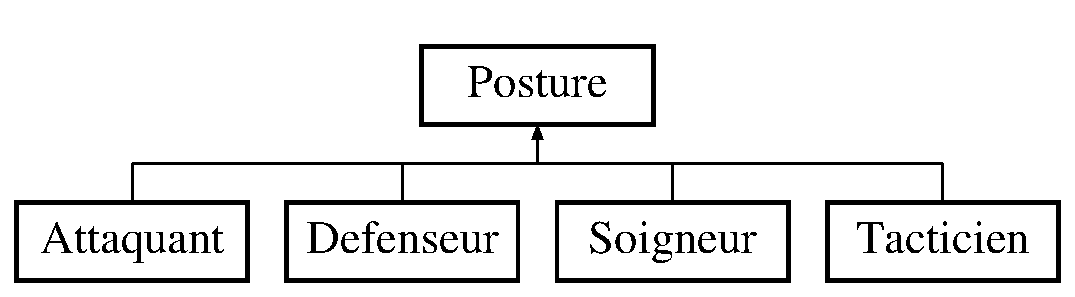
\includegraphics[height=2.000000cm]{classPosture}
\end{center}
\end{figure}
\subsection*{Fonctions membres publiques}
\begin{DoxyCompactItemize}
\item 
\hyperlink{classPosture_a926ec001a2ff5bf2577979a9804807dd}{Posture} (std\-::string nom\-Posture, int niveau)
\begin{DoxyCompactList}\small\item\em Constructeur de \hyperlink{classPosture}{Posture} (classe abstaite) \end{DoxyCompactList}\item 
\hypertarget{classPosture_ac7e7d04c473abd081d756dac19cbc778}{virtual \hyperlink{classPosture_ac7e7d04c473abd081d756dac19cbc778}{$\sim$\-Posture} ()=0}\label{classPosture_ac7e7d04c473abd081d756dac19cbc778}

\begin{DoxyCompactList}\small\item\em Destructeur de \hyperlink{classPosture}{Posture}. \end{DoxyCompactList}\item 
virtual int \hyperlink{classPosture_ae26355a91999a62fc528a73021e76d1f}{attaquer} (int degat)
\begin{DoxyCompactList}\small\item\em comportement de base d'attaque \end{DoxyCompactList}\item 
virtual int \hyperlink{classPosture_ab47310e905a5f6de83c945920f7c38b1}{soigner} (int soin)
\begin{DoxyCompactList}\small\item\em comportement de base de soigner \end{DoxyCompactList}\item 
virtual int \hyperlink{classPosture_a6c63571b8221847cf0abb1dce0ae1c5f}{subir\-Degat} (int degat)
\begin{DoxyCompactList}\small\item\em comportement de base de subir\-Degat \end{DoxyCompactList}\item 
virtual int \hyperlink{classPosture_a0988e92a33908186f74c44b54c1cb6db}{toucher} (int toucher)
\begin{DoxyCompactList}\small\item\em comportement de base de toucher \end{DoxyCompactList}\end{DoxyCompactItemize}
\subsection*{Attributs protégés}
\begin{DoxyCompactItemize}
\item 
\hypertarget{classPosture_a2630cb88d5c05164a9511bd93d40cbc6}{int {\bfseries niveau}}\label{classPosture_a2630cb88d5c05164a9511bd93d40cbc6}

\item 
\hypertarget{classPosture_a01479226a03454494774abf7330153d7}{std\-::string {\bfseries nom\-Posture}}\label{classPosture_a01479226a03454494774abf7330153d7}

\end{DoxyCompactItemize}


\subsection{Documentation des constructeurs et destructeur}
\hypertarget{classPosture_a926ec001a2ff5bf2577979a9804807dd}{\index{Posture@{Posture}!Posture@{Posture}}
\index{Posture@{Posture}!Posture@{Posture}}
\subsubsection[{Posture}]{\setlength{\rightskip}{0pt plus 5cm}Posture\-::\-Posture (
\begin{DoxyParamCaption}
\item[{std\-::string}]{nom\-Posture, }
\item[{int}]{niveau}
\end{DoxyParamCaption}
)}}\label{classPosture_a926ec001a2ff5bf2577979a9804807dd}


Constructeur de \hyperlink{classPosture}{Posture} (classe abstaite) 


\begin{DoxyParams}{Paramètres}
{\em n\-C} & std\-::string le nom de la \hyperlink{classPosture}{Posture} \\
\hline
{\em niveau} & int le niveau de la posture \\
\hline
\end{DoxyParams}


\subsection{Documentation des fonctions membres}
\hypertarget{classPosture_ae26355a91999a62fc528a73021e76d1f}{\index{Posture@{Posture}!attaquer@{attaquer}}
\index{attaquer@{attaquer}!Posture@{Posture}}
\subsubsection[{attaquer}]{\setlength{\rightskip}{0pt plus 5cm}int Posture\-::attaquer (
\begin{DoxyParamCaption}
\item[{int}]{degat}
\end{DoxyParamCaption}
)\hspace{0.3cm}{\ttfamily [virtual]}}}\label{classPosture_ae26355a91999a62fc528a73021e76d1f}


comportement de base d'attaque 


\begin{DoxyParams}{Paramètres}
{\em degat} & int les degats de base \\
\hline
\end{DoxyParams}
\begin{DoxyReturn}{Renvoie}
int les degats 
\end{DoxyReturn}


Réimplémentée dans \hyperlink{classTacticien_a2634b368edb2603afd2c1a76fdef8890}{Tacticien}, \hyperlink{classSoigneur_a94fa5f3bdffca0f474777d82a5f4b3e6}{Soigneur}, \hyperlink{classDefenseur_a9ec20f4bd6450776be10f4e9b037691d}{Defenseur}, et \hyperlink{classAttaquant_ad553f75cefdb44bf0703612940d597e4}{Attaquant}.

\hypertarget{classPosture_ab47310e905a5f6de83c945920f7c38b1}{\index{Posture@{Posture}!soigner@{soigner}}
\index{soigner@{soigner}!Posture@{Posture}}
\subsubsection[{soigner}]{\setlength{\rightskip}{0pt plus 5cm}int Posture\-::soigner (
\begin{DoxyParamCaption}
\item[{int}]{soin}
\end{DoxyParamCaption}
)\hspace{0.3cm}{\ttfamily [virtual]}}}\label{classPosture_ab47310e905a5f6de83c945920f7c38b1}


comportement de base de soigner 


\begin{DoxyParams}{Paramètres}
{\em soin} & int le nombre de pv soigner de base \\
\hline
\end{DoxyParams}
\begin{DoxyReturn}{Renvoie}
int les le nombre de pv soigner 
\end{DoxyReturn}


Réimplémentée dans \hyperlink{classSoigneur_a0f229f05071a0a2819906678f6fbaaae}{Soigneur}, et \hyperlink{classAttaquant_a874dc43af414df3c3c183e452f29a12a}{Attaquant}.

\hypertarget{classPosture_a6c63571b8221847cf0abb1dce0ae1c5f}{\index{Posture@{Posture}!subir\-Degat@{subir\-Degat}}
\index{subir\-Degat@{subir\-Degat}!Posture@{Posture}}
\subsubsection[{subir\-Degat}]{\setlength{\rightskip}{0pt plus 5cm}int Posture\-::subir\-Degat (
\begin{DoxyParamCaption}
\item[{int}]{degat}
\end{DoxyParamCaption}
)\hspace{0.3cm}{\ttfamily [virtual]}}}\label{classPosture_a6c63571b8221847cf0abb1dce0ae1c5f}


comportement de base de subir\-Degat 


\begin{DoxyParams}{Paramètres}
{\em degat} & int les degats de base \\
\hline
\end{DoxyParams}
\begin{DoxyReturn}{Renvoie}
int les degats 
\end{DoxyReturn}


Réimplémentée dans \hyperlink{classSoigneur_a7083e65720a01be6862ea640bf6d11c8}{Soigneur}, \hyperlink{classDefenseur_aa8a5e55f036a24005d9fab761d2ca272}{Defenseur}, et \hyperlink{classAttaquant_a3aeb7f6ca8b2397dd98bc52219aab836}{Attaquant}.

\hypertarget{classPosture_a0988e92a33908186f74c44b54c1cb6db}{\index{Posture@{Posture}!toucher@{toucher}}
\index{toucher@{toucher}!Posture@{Posture}}
\subsubsection[{toucher}]{\setlength{\rightskip}{0pt plus 5cm}int Posture\-::toucher (
\begin{DoxyParamCaption}
\item[{int}]{toucher}
\end{DoxyParamCaption}
)\hspace{0.3cm}{\ttfamily [virtual]}}}\label{classPosture_a0988e92a33908186f74c44b54c1cb6db}


comportement de base de toucher 


\begin{DoxyParams}{Paramètres}
{\em degat} & int le pourcentage de chance toucher de base \\
\hline
\end{DoxyParams}
\begin{DoxyReturn}{Renvoie}
int les le pourcentage de chance toucher de base 
\end{DoxyReturn}


Réimplémentée dans \hyperlink{classTacticien_a1aa0a98a2a29452ec7e61b132d348832}{Tacticien}, et \hyperlink{classAttaquant_adda67392faf5ffc39838a03168f1a591}{Attaquant}.



La documentation de cette classe a été générée à partir des fichiers suivants \-:\begin{DoxyCompactItemize}
\item 
Posture.\-hpp\item 
Posture.\-cpp\end{DoxyCompactItemize}

\hypertarget{classRace}{\section{Référence de la classe Race}
\label{classRace}\index{Race@{Race}}
}
\subsection*{Fonctions membres publiques}
\begin{DoxyCompactItemize}
\item 
\hyperlink{classRace_a1e548f6c42d50d34300dba2cf49c7213}{Race} (std\-::string n\-R, std\-::vector$<$ int $>$ m\-S)
\begin{DoxyCompactList}\small\item\em Constructeur de \hyperlink{classRace}{Race}. \end{DoxyCompactList}\item 
\hypertarget{classRace_ad6bfb0bc96485e23b3bf45d794b5b536}{\hyperlink{classRace_ad6bfb0bc96485e23b3bf45d794b5b536}{$\sim$\-Race} ()}\label{classRace_ad6bfb0bc96485e23b3bf45d794b5b536}

\begin{DoxyCompactList}\small\item\em Destructeur de \hyperlink{classRace}{Race}. \end{DoxyCompactList}\item 
std\-::vector$<$ int $>$ \hyperlink{classRace_a7f37cf16b2eaaca794a77d573952fbfc}{getmodificateur\-Statistique} ()
\begin{DoxyCompactList}\small\item\em getter du vector$<$sting$>$ de modificateur de stat de la \hyperlink{classRace}{Race} \end{DoxyCompactList}\item 
std\-::string \hyperlink{classRace_aa5ff2e9b3f7208508da1263fb862d1c0}{getmodificateur\-Statistique\-String} ()
\begin{DoxyCompactList}\small\item\em retour le vector$<$sting$>$ de modificateur de stat de la \hyperlink{classRace}{Race} sous la forme d'une string \end{DoxyCompactList}\item 
std\-::string \hyperlink{classRace_afb43932eb39516f1d199843edd2999df}{get\-Nom\-Race} ()
\begin{DoxyCompactList}\small\item\em getter du nom de la \hyperlink{classRace}{Race} \end{DoxyCompactList}\end{DoxyCompactItemize}


\subsection{Documentation des constructeurs et destructeur}
\hypertarget{classRace_a1e548f6c42d50d34300dba2cf49c7213}{\index{Race@{Race}!Race@{Race}}
\index{Race@{Race}!Race@{Race}}
\subsubsection[{Race}]{\setlength{\rightskip}{0pt plus 5cm}Race\-::\-Race (
\begin{DoxyParamCaption}
\item[{std\-::string}]{n\-R, }
\item[{std\-::vector$<$ int $>$}]{m\-S}
\end{DoxyParamCaption}
)}}\label{classRace_a1e548f6c42d50d34300dba2cf49c7213}


Constructeur de \hyperlink{classRace}{Race}. 


\begin{DoxyParams}{Paramètres}
{\em n\-R} & std\-::string Le nom de la race. \\
\hline
{\em m\-S} & std\-::vector$<$int$>$ Le vector de stat de la race \\
\hline
\end{DoxyParams}


\subsection{Documentation des fonctions membres}
\hypertarget{classRace_a7f37cf16b2eaaca794a77d573952fbfc}{\index{Race@{Race}!getmodificateur\-Statistique@{getmodificateur\-Statistique}}
\index{getmodificateur\-Statistique@{getmodificateur\-Statistique}!Race@{Race}}
\subsubsection[{getmodificateur\-Statistique}]{\setlength{\rightskip}{0pt plus 5cm}std\-::vector$<$ int $>$ Race\-::getmodificateur\-Statistique (
\begin{DoxyParamCaption}
{}
\end{DoxyParamCaption}
)}}\label{classRace_a7f37cf16b2eaaca794a77d573952fbfc}


getter du vector$<$sting$>$ de modificateur de stat de la \hyperlink{classRace}{Race} 

\begin{DoxyReturn}{Renvoie}
std\-::vector$<$sting$>$ de modificateur de stat de la \hyperlink{classRace}{Race} 
\end{DoxyReturn}
\hypertarget{classRace_aa5ff2e9b3f7208508da1263fb862d1c0}{\index{Race@{Race}!getmodificateur\-Statistique\-String@{getmodificateur\-Statistique\-String}}
\index{getmodificateur\-Statistique\-String@{getmodificateur\-Statistique\-String}!Race@{Race}}
\subsubsection[{getmodificateur\-Statistique\-String}]{\setlength{\rightskip}{0pt plus 5cm}std\-::string Race\-::getmodificateur\-Statistique\-String (
\begin{DoxyParamCaption}
{}
\end{DoxyParamCaption}
)}}\label{classRace_aa5ff2e9b3f7208508da1263fb862d1c0}


retour le vector$<$sting$>$ de modificateur de stat de la \hyperlink{classRace}{Race} sous la forme d'une string 

\begin{DoxyReturn}{Renvoie}
std\-::sting le vector$<$sting$>$ de modificateur de stat de la \hyperlink{classRace}{Race} en string 
\end{DoxyReturn}
\hypertarget{classRace_afb43932eb39516f1d199843edd2999df}{\index{Race@{Race}!get\-Nom\-Race@{get\-Nom\-Race}}
\index{get\-Nom\-Race@{get\-Nom\-Race}!Race@{Race}}
\subsubsection[{get\-Nom\-Race}]{\setlength{\rightskip}{0pt plus 5cm}std\-::string Race\-::get\-Nom\-Race (
\begin{DoxyParamCaption}
{}
\end{DoxyParamCaption}
)}}\label{classRace_afb43932eb39516f1d199843edd2999df}


getter du nom de la \hyperlink{classRace}{Race} 

\begin{DoxyReturn}{Renvoie}
std\-::string le nom de la race 
\end{DoxyReturn}


La documentation de cette classe a été générée à partir des fichiers suivants \-:\begin{DoxyCompactItemize}
\item 
Race.\-hpp\item 
Race.\-cpp\end{DoxyCompactItemize}

\hypertarget{classSoigneur}{\section{Référence de la classe Soigneur}
\label{classSoigneur}\index{Soigneur@{Soigneur}}
}
Graphe d'héritage de Soigneur\-:\begin{figure}[H]
\begin{center}
\leavevmode
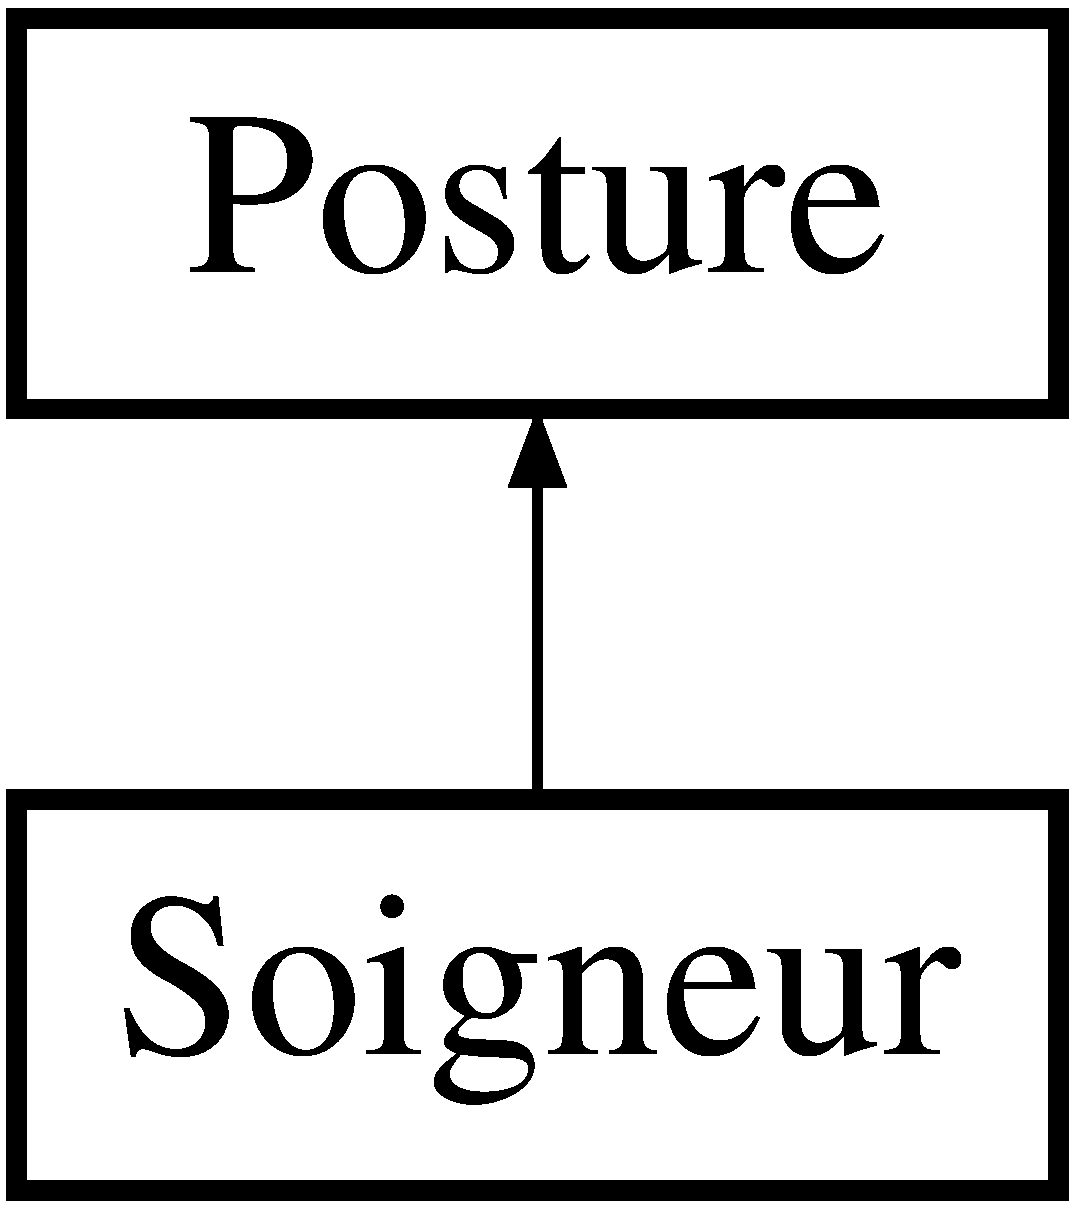
\includegraphics[height=2.000000cm]{classSoigneur}
\end{center}
\end{figure}
\subsection*{Fonctions membres publiques}
\begin{DoxyCompactItemize}
\item 
\hyperlink{classSoigneur_a1b2ad1c5e5b338bb4ef75d137a81e290}{Soigneur} (int niveau)
\begin{DoxyCompactList}\small\item\em Constructeur de \hyperlink{classSoigneur}{Soigneur} herite de \hyperlink{classPosture}{Posture}. \end{DoxyCompactList}\item 
\hypertarget{classSoigneur_ab2c59b538fee3f08fda30fcc8cc5449b}{\hyperlink{classSoigneur_ab2c59b538fee3f08fda30fcc8cc5449b}{$\sim$\-Soigneur} ()}\label{classSoigneur_ab2c59b538fee3f08fda30fcc8cc5449b}

\begin{DoxyCompactList}\small\item\em Destructeur de \hyperlink{classSoigneur}{Soigneur}. \end{DoxyCompactList}\item 
int \hyperlink{classSoigneur_a94fa5f3bdffca0f474777d82a5f4b3e6}{attaquer} (int degat)
\begin{DoxyCompactList}\small\item\em comportement d'attaque de \hyperlink{classSoigneur}{Soigneur} \end{DoxyCompactList}\item 
int \hyperlink{classSoigneur_a7083e65720a01be6862ea640bf6d11c8}{subir\-Degat} (int degat)
\begin{DoxyCompactList}\small\item\em comportement de subir\-Degat en \hyperlink{classSoigneur}{Soigneur} \end{DoxyCompactList}\item 
int \hyperlink{classSoigneur_a0f229f05071a0a2819906678f6fbaaae}{soigner} (int soin)
\begin{DoxyCompactList}\small\item\em comportement de se soigner en \hyperlink{classSoigneur}{Soigneur} \end{DoxyCompactList}\end{DoxyCompactItemize}
\subsection*{Membres hérités additionnels}


\subsection{Documentation des constructeurs et destructeur}
\hypertarget{classSoigneur_a1b2ad1c5e5b338bb4ef75d137a81e290}{\index{Soigneur@{Soigneur}!Soigneur@{Soigneur}}
\index{Soigneur@{Soigneur}!Soigneur@{Soigneur}}
\subsubsection[{Soigneur}]{\setlength{\rightskip}{0pt plus 5cm}Soigneur\-::\-Soigneur (
\begin{DoxyParamCaption}
\item[{int}]{niveau}
\end{DoxyParamCaption}
)}}\label{classSoigneur_a1b2ad1c5e5b338bb4ef75d137a81e290}


Constructeur de \hyperlink{classSoigneur}{Soigneur} herite de \hyperlink{classPosture}{Posture}. 


\begin{DoxyParams}{Paramètres}
{\em niveau} & int le niveau de la posture \\
\hline
\end{DoxyParams}


\subsection{Documentation des fonctions membres}
\hypertarget{classSoigneur_a94fa5f3bdffca0f474777d82a5f4b3e6}{\index{Soigneur@{Soigneur}!attaquer@{attaquer}}
\index{attaquer@{attaquer}!Soigneur@{Soigneur}}
\subsubsection[{attaquer}]{\setlength{\rightskip}{0pt plus 5cm}int Soigneur\-::attaquer (
\begin{DoxyParamCaption}
\item[{int}]{degat}
\end{DoxyParamCaption}
)\hspace{0.3cm}{\ttfamily [virtual]}}}\label{classSoigneur_a94fa5f3bdffca0f474777d82a5f4b3e6}


comportement d'attaque de \hyperlink{classSoigneur}{Soigneur} 


\begin{DoxyParams}{Paramètres}
{\em degat} & int les degats de base \\
\hline
\end{DoxyParams}
\begin{DoxyReturn}{Renvoie}
int les degats 
\end{DoxyReturn}


Réimplémentée à partir de \hyperlink{classPosture_ae26355a91999a62fc528a73021e76d1f}{Posture}.

\hypertarget{classSoigneur_a0f229f05071a0a2819906678f6fbaaae}{\index{Soigneur@{Soigneur}!soigner@{soigner}}
\index{soigner@{soigner}!Soigneur@{Soigneur}}
\subsubsection[{soigner}]{\setlength{\rightskip}{0pt plus 5cm}int Soigneur\-::soigner (
\begin{DoxyParamCaption}
\item[{int}]{soin}
\end{DoxyParamCaption}
)\hspace{0.3cm}{\ttfamily [virtual]}}}\label{classSoigneur_a0f229f05071a0a2819906678f6fbaaae}


comportement de se soigner en \hyperlink{classSoigneur}{Soigneur} 


\begin{DoxyParams}{Paramètres}
{\em soin} & int le nombre de pv soigner de base \\
\hline
\end{DoxyParams}
\begin{DoxyReturn}{Renvoie}
int les le nombre de pv soigner 
\end{DoxyReturn}


Réimplémentée à partir de \hyperlink{classPosture_ab47310e905a5f6de83c945920f7c38b1}{Posture}.

\hypertarget{classSoigneur_a7083e65720a01be6862ea640bf6d11c8}{\index{Soigneur@{Soigneur}!subir\-Degat@{subir\-Degat}}
\index{subir\-Degat@{subir\-Degat}!Soigneur@{Soigneur}}
\subsubsection[{subir\-Degat}]{\setlength{\rightskip}{0pt plus 5cm}int Soigneur\-::subir\-Degat (
\begin{DoxyParamCaption}
\item[{int}]{degat}
\end{DoxyParamCaption}
)\hspace{0.3cm}{\ttfamily [virtual]}}}\label{classSoigneur_a7083e65720a01be6862ea640bf6d11c8}


comportement de subir\-Degat en \hyperlink{classSoigneur}{Soigneur} 


\begin{DoxyParams}{Paramètres}
{\em degat} & int les degats de base \\
\hline
\end{DoxyParams}
\begin{DoxyReturn}{Renvoie}
int les degats 
\end{DoxyReturn}


Réimplémentée à partir de \hyperlink{classPosture_a6c63571b8221847cf0abb1dce0ae1c5f}{Posture}.



La documentation de cette classe a été générée à partir des fichiers suivants \-:\begin{DoxyCompactItemize}
\item 
Posture.\-hpp\item 
Posture.\-cpp\end{DoxyCompactItemize}

\hypertarget{classSort}{\section{Référence de la classe Sort}
\label{classSort}\index{Sort@{Sort}}
}
Graphe d'héritage de Sort\-:\begin{figure}[H]
\begin{center}
\leavevmode
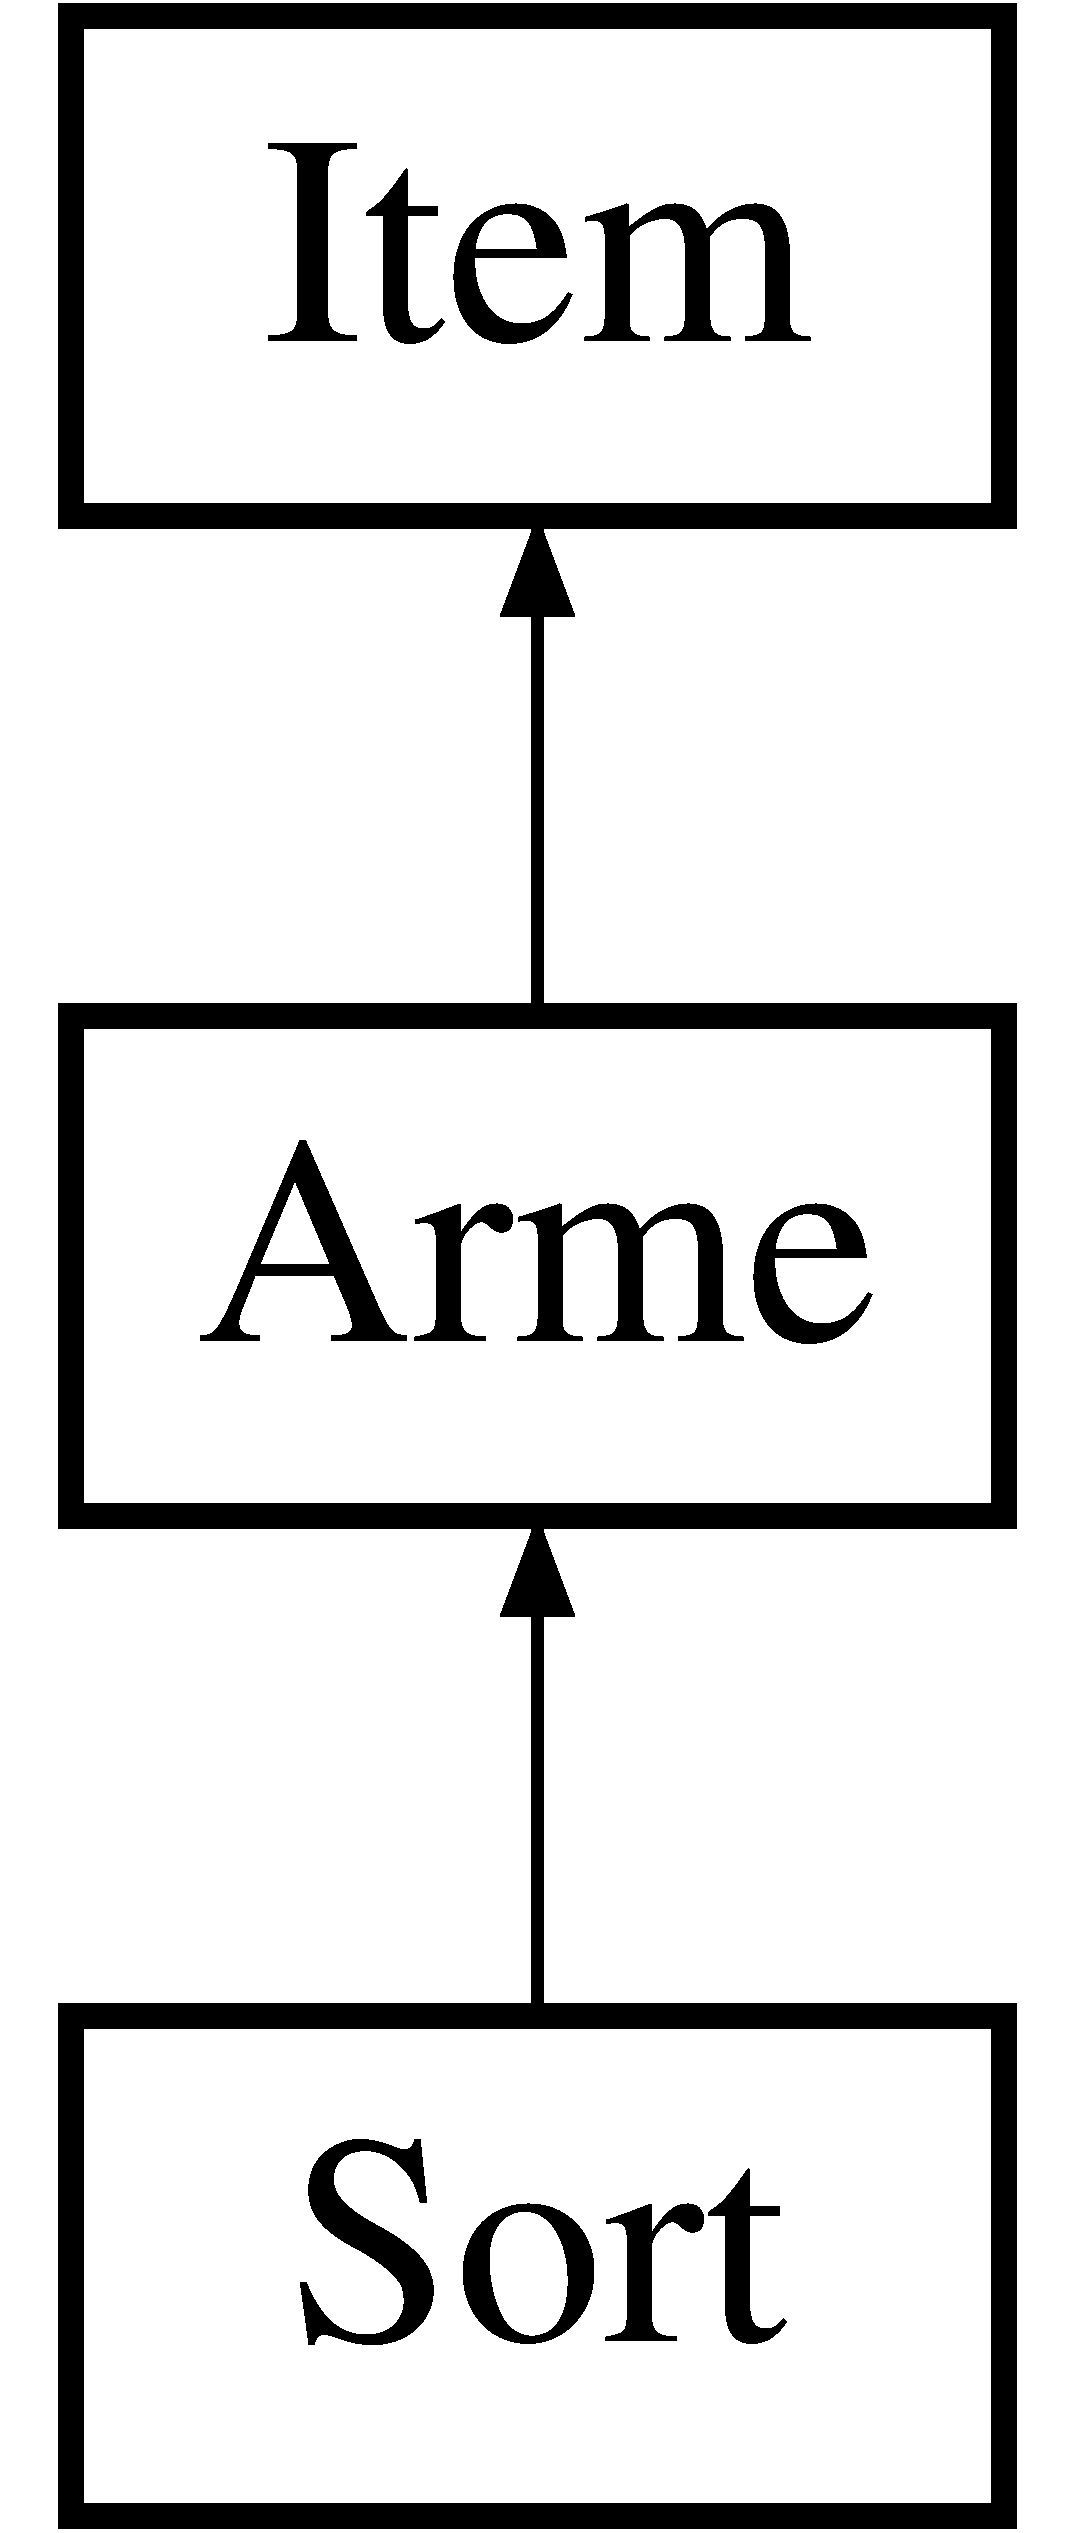
\includegraphics[height=3.000000cm]{classSort}
\end{center}
\end{figure}
\subsection*{Fonctions membres publiques}
\begin{DoxyCompactItemize}
\item 
\hypertarget{classSort_aa71bc58371a3504b076042269d2b9827}{\hyperlink{classSort_aa71bc58371a3504b076042269d2b9827}{Sort} (std\-::string nom\-Arme, int puissance, int precision, int critique, bool est\-Magique, int prix)}\label{classSort_aa71bc58371a3504b076042269d2b9827}

\begin{DoxyCompactList}\small\item\em Construit une arme de type 2. \end{DoxyCompactList}\end{DoxyCompactItemize}
\subsection*{Membres hérités additionnels}


La documentation de cette classe a été générée à partir des fichiers suivants \-:\begin{DoxyCompactItemize}
\item 
Armes.\-hpp\item 
Armes.\-cpp\end{DoxyCompactItemize}

\hypertarget{classTacticien}{\section{Référence de la classe Tacticien}
\label{classTacticien}\index{Tacticien@{Tacticien}}
}
Graphe d'héritage de Tacticien\-:\begin{figure}[H]
\begin{center}
\leavevmode
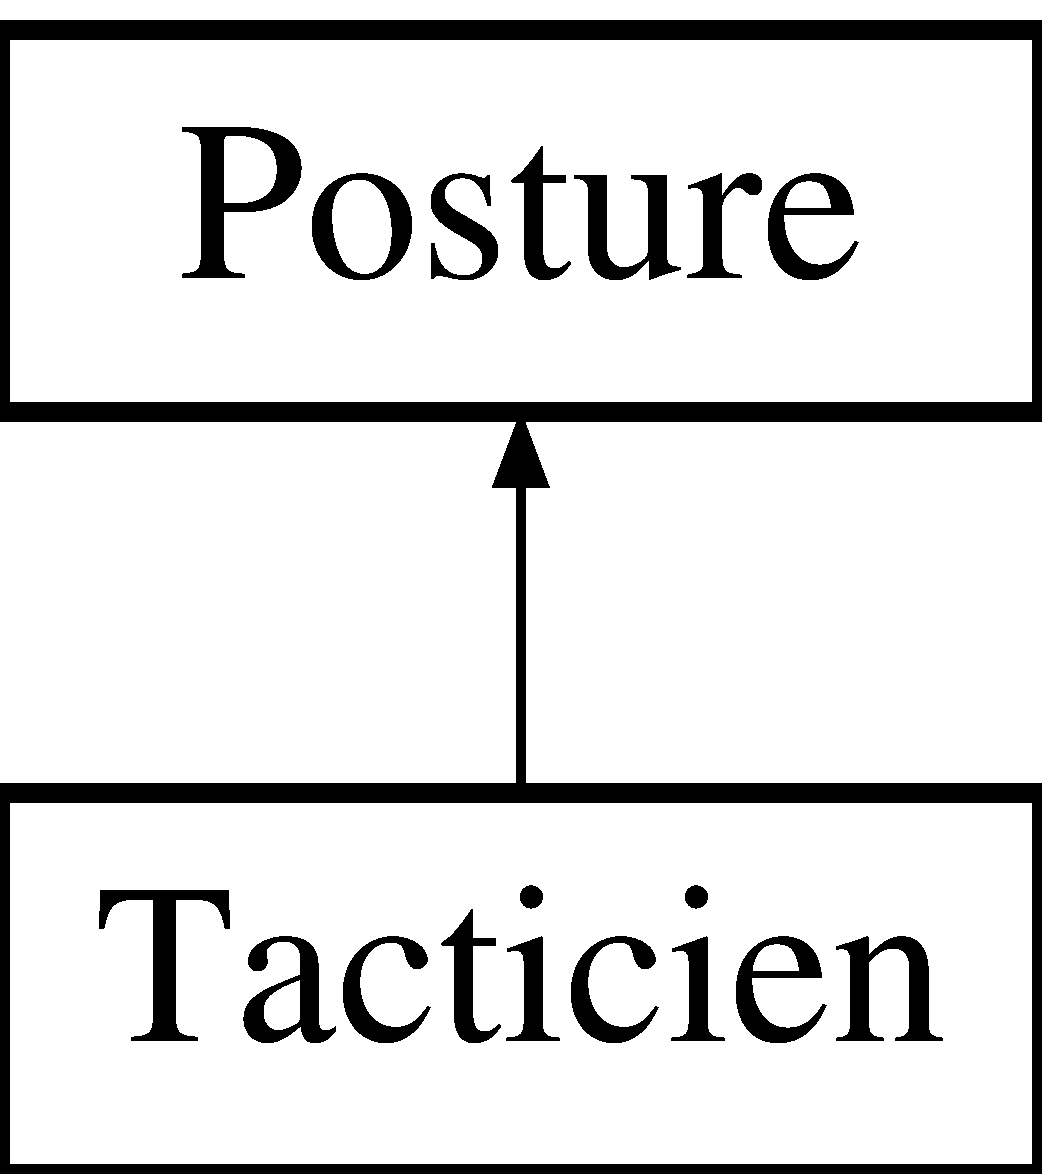
\includegraphics[height=2.000000cm]{classTacticien}
\end{center}
\end{figure}
\subsection*{Fonctions membres publiques}
\begin{DoxyCompactItemize}
\item 
\hyperlink{classTacticien_aafeab917c80abe90da1f97b33a946c5d}{Tacticien} (int niveau)
\begin{DoxyCompactList}\small\item\em Constructeur de \hyperlink{classTacticien}{Tacticien} herite de \hyperlink{classPosture}{Posture}. \end{DoxyCompactList}\item 
\hypertarget{classTacticien_a82d1dcd43e8d66ef380d70e33e0f3030}{\hyperlink{classTacticien_a82d1dcd43e8d66ef380d70e33e0f3030}{$\sim$\-Tacticien} ()}\label{classTacticien_a82d1dcd43e8d66ef380d70e33e0f3030}

\begin{DoxyCompactList}\small\item\em Destructeur de \hyperlink{classTacticien}{Tacticien}. \end{DoxyCompactList}\item 
int \hyperlink{classTacticien_a2634b368edb2603afd2c1a76fdef8890}{attaquer} (int degat)
\begin{DoxyCompactList}\small\item\em comportement d'attaque de \hyperlink{classTacticien}{Tacticien} \end{DoxyCompactList}\item 
int \hyperlink{classTacticien_a1aa0a98a2a29452ec7e61b132d348832}{toucher} (int toucher)
\begin{DoxyCompactList}\small\item\em comportement de toucher en \hyperlink{classTacticien}{Tacticien} \end{DoxyCompactList}\end{DoxyCompactItemize}
\subsection*{Membres hérités additionnels}


\subsection{Documentation des constructeurs et destructeur}
\hypertarget{classTacticien_aafeab917c80abe90da1f97b33a946c5d}{\index{Tacticien@{Tacticien}!Tacticien@{Tacticien}}
\index{Tacticien@{Tacticien}!Tacticien@{Tacticien}}
\subsubsection[{Tacticien}]{\setlength{\rightskip}{0pt plus 5cm}Tacticien\-::\-Tacticien (
\begin{DoxyParamCaption}
\item[{int}]{niveau}
\end{DoxyParamCaption}
)}}\label{classTacticien_aafeab917c80abe90da1f97b33a946c5d}


Constructeur de \hyperlink{classTacticien}{Tacticien} herite de \hyperlink{classPosture}{Posture}. 


\begin{DoxyParams}{Paramètres}
{\em niveau} & int le niveau de la posture \\
\hline
\end{DoxyParams}


\subsection{Documentation des fonctions membres}
\hypertarget{classTacticien_a2634b368edb2603afd2c1a76fdef8890}{\index{Tacticien@{Tacticien}!attaquer@{attaquer}}
\index{attaquer@{attaquer}!Tacticien@{Tacticien}}
\subsubsection[{attaquer}]{\setlength{\rightskip}{0pt plus 5cm}int Tacticien\-::attaquer (
\begin{DoxyParamCaption}
\item[{int}]{degat}
\end{DoxyParamCaption}
)\hspace{0.3cm}{\ttfamily [virtual]}}}\label{classTacticien_a2634b368edb2603afd2c1a76fdef8890}


comportement d'attaque de \hyperlink{classTacticien}{Tacticien} 


\begin{DoxyParams}{Paramètres}
{\em degat} & int les degats de base \\
\hline
\end{DoxyParams}
\begin{DoxyReturn}{Renvoie}
int les degats 
\end{DoxyReturn}


Réimplémentée à partir de \hyperlink{classPosture_ae26355a91999a62fc528a73021e76d1f}{Posture}.

\hypertarget{classTacticien_a1aa0a98a2a29452ec7e61b132d348832}{\index{Tacticien@{Tacticien}!toucher@{toucher}}
\index{toucher@{toucher}!Tacticien@{Tacticien}}
\subsubsection[{toucher}]{\setlength{\rightskip}{0pt plus 5cm}int Tacticien\-::toucher (
\begin{DoxyParamCaption}
\item[{int}]{toucher}
\end{DoxyParamCaption}
)\hspace{0.3cm}{\ttfamily [virtual]}}}\label{classTacticien_a1aa0a98a2a29452ec7e61b132d348832}


comportement de toucher en \hyperlink{classTacticien}{Tacticien} 


\begin{DoxyParams}{Paramètres}
{\em degat} & int le pourcentage de chance toucher de base \\
\hline
\end{DoxyParams}
\begin{DoxyReturn}{Renvoie}
int les le pourcentage de chance toucher de base 
\end{DoxyReturn}


Réimplémentée à partir de \hyperlink{classPosture_a0988e92a33908186f74c44b54c1cb6db}{Posture}.



La documentation de cette classe a été générée à partir des fichiers suivants \-:\begin{DoxyCompactItemize}
\item 
Posture.\-hpp\item 
Posture.\-cpp\end{DoxyCompactItemize}

\hypertarget{classTechnique}{\section{Référence de la classe Technique}
\label{classTechnique}\index{Technique@{Technique}}
}
Graphe d'héritage de Technique\-:\begin{figure}[H]
\begin{center}
\leavevmode
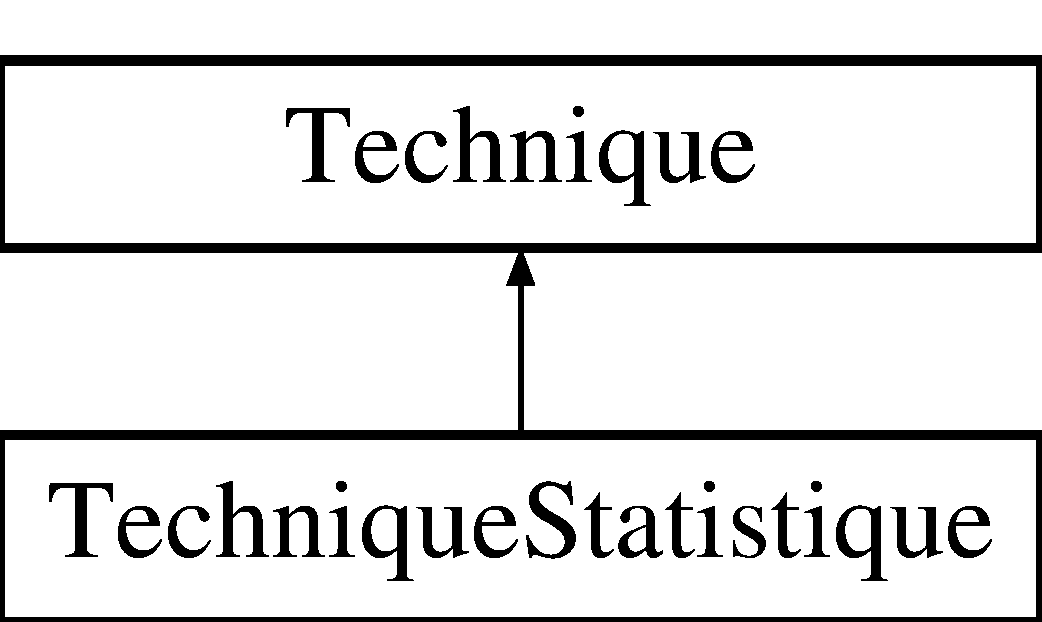
\includegraphics[height=2.000000cm]{classTechnique}
\end{center}
\end{figure}
\subsection*{Fonctions membres publiques}
\begin{DoxyCompactItemize}
\item 
\hyperlink{classTechnique_a48988caf322c83fbc5596790f068a69b}{Technique} (std\-::string nom\-T)
\begin{DoxyCompactList}\small\item\em Constructeur de \hyperlink{classTechnique}{Technique} (classe abstaite) \end{DoxyCompactList}\item 
\hypertarget{classTechnique_a98e31009f87eaf1971145162254ef8ae}{virtual \hyperlink{classTechnique_a98e31009f87eaf1971145162254ef8ae}{$\sim$\-Technique} ()=0}\label{classTechnique_a98e31009f87eaf1971145162254ef8ae}

\begin{DoxyCompactList}\small\item\em Destructeur de \hyperlink{classTechnique}{Technique}. \end{DoxyCompactList}\item 
std\-::string \hyperlink{classTechnique_abc365297482e838ddc01804619590a15}{get\-Nom\-Technique} ()
\begin{DoxyCompactList}\small\item\em getter du nom de la \hyperlink{classTechnique}{Technique} \end{DoxyCompactList}\end{DoxyCompactItemize}
\subsection*{Attributs protégés}
\begin{DoxyCompactItemize}
\item 
\hypertarget{classTechnique_a4f7663af14f4954d0d22efdcc1f1b070}{std\-::string {\bfseries nom\-Technique}}\label{classTechnique_a4f7663af14f4954d0d22efdcc1f1b070}

\end{DoxyCompactItemize}


\subsection{Documentation des constructeurs et destructeur}
\hypertarget{classTechnique_a48988caf322c83fbc5596790f068a69b}{\index{Technique@{Technique}!Technique@{Technique}}
\index{Technique@{Technique}!Technique@{Technique}}
\subsubsection[{Technique}]{\setlength{\rightskip}{0pt plus 5cm}Technique\-::\-Technique (
\begin{DoxyParamCaption}
\item[{std\-::string}]{nom\-T}
\end{DoxyParamCaption}
)}}\label{classTechnique_a48988caf322c83fbc5596790f068a69b}


Constructeur de \hyperlink{classTechnique}{Technique} (classe abstaite) 


\begin{DoxyParams}{Paramètres}
{\em nom\-T} & std\-::string le nom de la \hyperlink{classTechnique}{Technique} \\
\hline
\end{DoxyParams}


\subsection{Documentation des fonctions membres}
\hypertarget{classTechnique_abc365297482e838ddc01804619590a15}{\index{Technique@{Technique}!get\-Nom\-Technique@{get\-Nom\-Technique}}
\index{get\-Nom\-Technique@{get\-Nom\-Technique}!Technique@{Technique}}
\subsubsection[{get\-Nom\-Technique}]{\setlength{\rightskip}{0pt plus 5cm}std\-::string Technique\-::get\-Nom\-Technique (
\begin{DoxyParamCaption}
{}
\end{DoxyParamCaption}
)}}\label{classTechnique_abc365297482e838ddc01804619590a15}


getter du nom de la \hyperlink{classTechnique}{Technique} 

\begin{DoxyReturn}{Renvoie}
std\-::string le nom de la \hyperlink{classTechnique}{Technique} 
\end{DoxyReturn}


La documentation de cette classe a été générée à partir des fichiers suivants \-:\begin{DoxyCompactItemize}
\item 
Technique.\-hpp\item 
Technique.\-cpp\end{DoxyCompactItemize}

\hypertarget{classTechniqueStatistique}{\section{Référence de la classe Technique\-Statistique}
\label{classTechniqueStatistique}\index{Technique\-Statistique@{Technique\-Statistique}}
}
Graphe d'héritage de Technique\-Statistique\-:\begin{figure}[H]
\begin{center}
\leavevmode
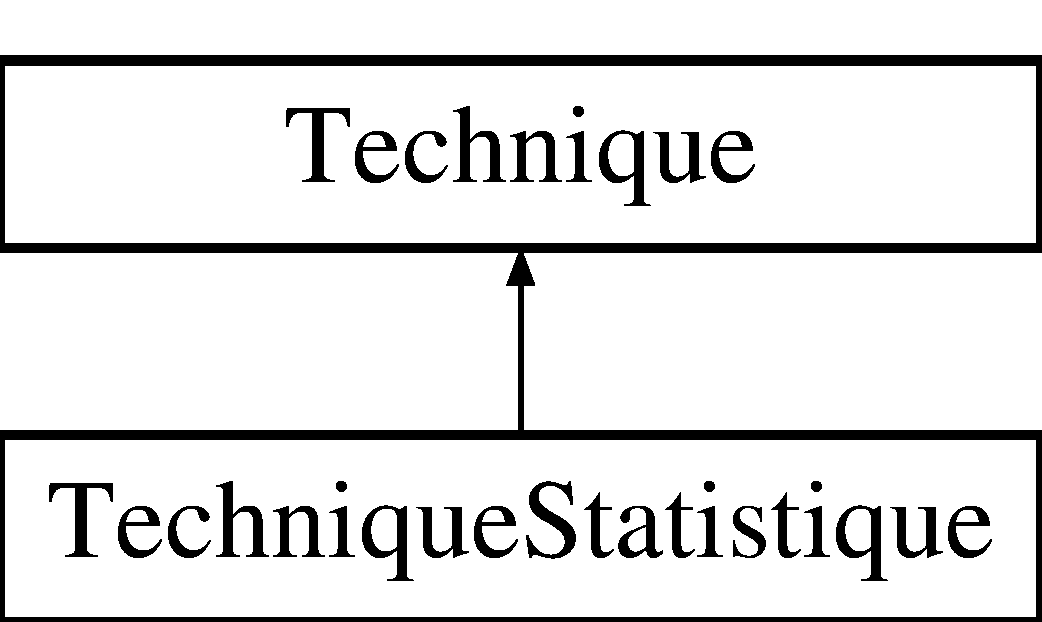
\includegraphics[height=2.000000cm]{classTechniqueStatistique}
\end{center}
\end{figure}
\subsection*{Fonctions membres publiques}
\begin{DoxyCompactItemize}
\item 
\hyperlink{classTechniqueStatistique_aae9fc24bfe4041589a6db6d13139a157}{Technique\-Statistique} (std\-::string nom\-T, int s)
\begin{DoxyCompactList}\small\item\em Constructeur de \hyperlink{classTechniqueStatistique}{Technique\-Statistique}. \end{DoxyCompactList}\item 
\hypertarget{classTechniqueStatistique_a92d43e32d7ff83eb97e00388dc10efc2}{\hyperlink{classTechniqueStatistique_a92d43e32d7ff83eb97e00388dc10efc2}{$\sim$\-Technique\-Statistique} ()}\label{classTechniqueStatistique_a92d43e32d7ff83eb97e00388dc10efc2}

\begin{DoxyCompactList}\small\item\em Destructeur de \hyperlink{classTechniqueStatistique}{Technique\-Statistique}. \end{DoxyCompactList}\item 
int \hyperlink{classTechniqueStatistique_aca07b10c097c294e45c3c35d3966e7c2}{get\-Stat\-To\-Up} ()
\begin{DoxyCompactList}\small\item\em getter de stat\-To\-Up \end{DoxyCompactList}\end{DoxyCompactItemize}
\subsection*{Membres hérités additionnels}


\subsection{Documentation des constructeurs et destructeur}
\hypertarget{classTechniqueStatistique_aae9fc24bfe4041589a6db6d13139a157}{\index{Technique\-Statistique@{Technique\-Statistique}!Technique\-Statistique@{Technique\-Statistique}}
\index{Technique\-Statistique@{Technique\-Statistique}!TechniqueStatistique@{Technique\-Statistique}}
\subsubsection[{Technique\-Statistique}]{\setlength{\rightskip}{0pt plus 5cm}Technique\-Statistique\-::\-Technique\-Statistique (
\begin{DoxyParamCaption}
\item[{std\-::string}]{nom\-T, }
\item[{int}]{s}
\end{DoxyParamCaption}
)}}\label{classTechniqueStatistique_aae9fc24bfe4041589a6db6d13139a157}


Constructeur de \hyperlink{classTechniqueStatistique}{Technique\-Statistique}. 


\begin{DoxyParams}{Paramètres}
{\em nom\-T} & std\-::string le nom de la \hyperlink{classTechnique}{Technique} \\
\hline
{\em s} & int la stat a ameliorer \\
\hline
\end{DoxyParams}


\subsection{Documentation des fonctions membres}
\hypertarget{classTechniqueStatistique_aca07b10c097c294e45c3c35d3966e7c2}{\index{Technique\-Statistique@{Technique\-Statistique}!get\-Stat\-To\-Up@{get\-Stat\-To\-Up}}
\index{get\-Stat\-To\-Up@{get\-Stat\-To\-Up}!TechniqueStatistique@{Technique\-Statistique}}
\subsubsection[{get\-Stat\-To\-Up}]{\setlength{\rightskip}{0pt plus 5cm}int Technique\-Statistique\-::get\-Stat\-To\-Up (
\begin{DoxyParamCaption}
{}
\end{DoxyParamCaption}
)}}\label{classTechniqueStatistique_aca07b10c097c294e45c3c35d3966e7c2}


getter de stat\-To\-Up 

\begin{DoxyReturn}{Renvoie}
int la stat a ameliorer 
\end{DoxyReturn}


La documentation de cette classe a été générée à partir des fichiers suivants \-:\begin{DoxyCompactItemize}
\item 
Technique.\-hpp\item 
Technique.\-cpp\end{DoxyCompactItemize}

%--- End generated contents ---

% Index
\newpage
\phantomsection
\addcontentsline{toc}{chapter}{Index}
\printindex

\end{document}
